\documentclass[11pt]{beamer}
\usetheme[sectionpage=none, progressbar=frametitle]{metropolis}
\usecolortheme{beaver}
\usepackage[utf8]{inputenc}
\usepackage{amsmath}
\usepackage{amsfonts}
\usepackage{amssymb}
\usepackage{url}
\usepackage{relsize}
\usepackage{graphicx}
\usepackage{comment}

\usepackage[breakable, theorems, skins]{tcolorbox}
\tcbset{enhanced}
\usepackage{appendixnumberbeamer}
\newcommand{\gap}{\\[2ex]}
\setbeamertemplate{footline}[frame number]
\DeclareRobustCommand{\myboxright}[2][gray!20]{%
\begin{tcolorbox}[
        left=0pt,
        right=0pt,
        top=0pt,
        bottom=0pt,
        colback=#1,
        colframe=#1,
        width=0.32\textwidth, 
        enlarge left by=75mm,
        enlarge top by=29mm,
        boxsep=0pt,
        arc=0pt,outer arc=5pt,
        ]
        #2
\end{tcolorbox}
}
\DeclareRobustCommand{\mybox}[2][gray!20]{%
\begin{tcolorbox}[
        left=0pt,
        right=0pt,
        top=0pt,
        bottom=0pt,
        colback=#1,
        colframe=#1,
        width=\dimexpr\textwidth\relax, 
        enlarge left by=0mm,
        boxsep=0pt,
        arc=0pt,outer arc=5pt,
        ]
        #2
\end{tcolorbox}
}
\newcommand\blfootnote[1]{%
  \begingroup
  \renewcommand\thefootnote{}\footnote{#1}%
  \addtocounter{footnote}{-1}%
  \endgroup
}

\begin{document}




\title{lowEBMs: A Python implementation of low-dimensional energy balance models}

\subtitle{Application example: Late Holocene temperature response}

\author{Benjamin Schmiedel}


\institute[UHD] % (optional)
{
  Institute of Environmental Physics\\
  University of Heidelberg
  \and
  Geophysical Institute\\
  University of Bergen
}

\date{19.08.2019} 

\begin{frame}
	\tikz [remember picture,overlay]
    	\node[xshift=3cm,yshift=-2.5cm] at (current page.center) {
\includegraphics[width=0.5\textwidth]{Figures/Logos/Logo_big.png}};
    \tikz [remember picture,overlay]		
    	\node[xshift=5.15cm, yshift=4.35cm] at (current page.center) {
\includegraphics[width=0.2\textwidth]{Figures/Logos/bjerkneslogo_big.png}};
    \titlepage
\end{frame}

\section{Motivation}

\begin{frame}{Motivation - STACY Group}
    \begin{tikzpicture}[remember picture,overlay]
%    \node[xshift=0cm, yshift=-1.5cm] at (current page.center) {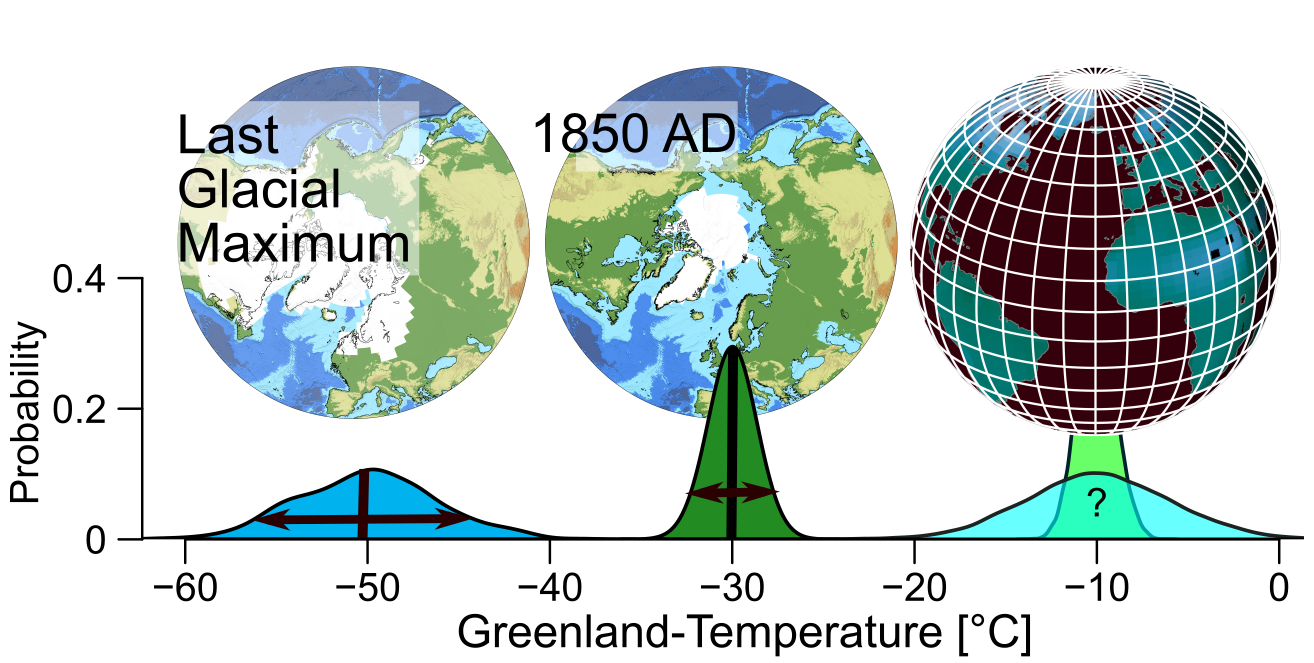
\includegraphics[width=\textwidth]{Figures/Motivation/Stacy_density_title.png}};
    \node[xshift=0cm, yshift=-1.2cm] at (current page.center) {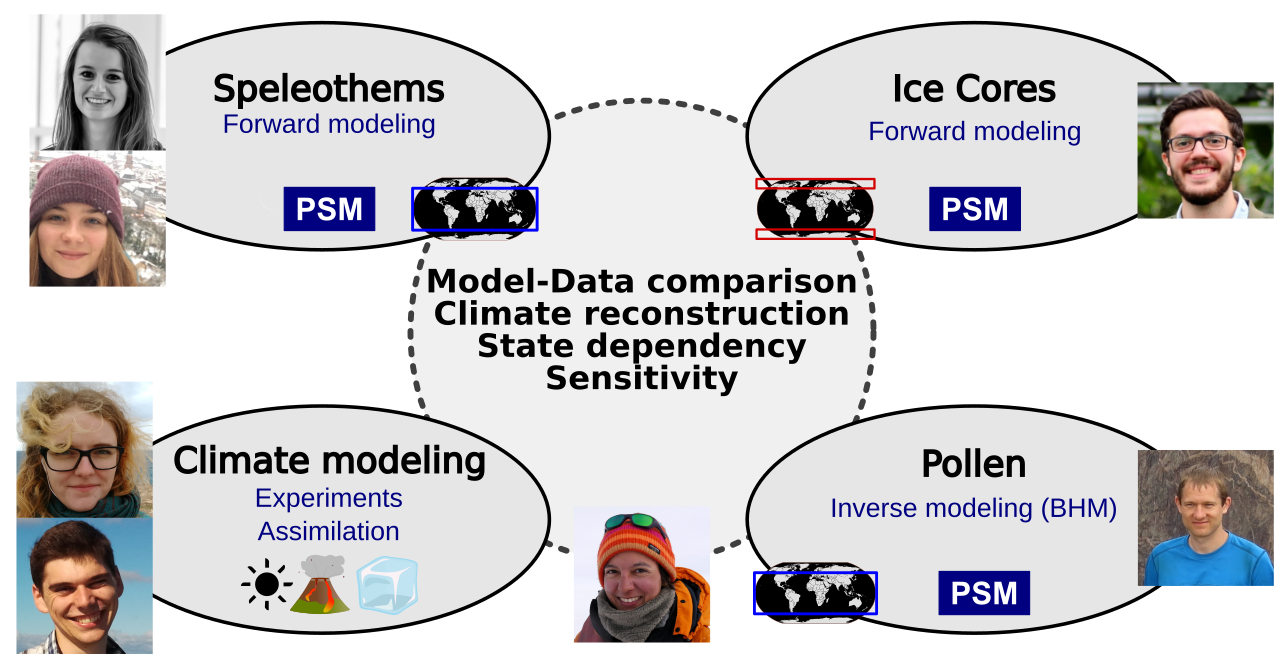
\includegraphics[width=1.1\textwidth]{Figures/Motivation/stacy_group_2.png}};

    %\node[draw,xshift=-0.35cm,yshift=-2.2cm] at (current page.45) {
\includegraphics[width=0.3\textwidth]{Figures/Logos/Stacy_logo.png}};
    \node[xshift=0cm,yshift=2.8cm] at (current page.center) {
\includegraphics[width=0.3\textwidth]{Figures/Logos/Stacy_logo.png}};
    \node[xshift=4.4cm, yshift=4.3cm] at (current page.center) {
\includegraphics[width=0.08\textwidth]{Figures/Logos/LogoIUP.png}};
    \node[xshift=3.4cm, yshift=4.3cm] at (current page.center) {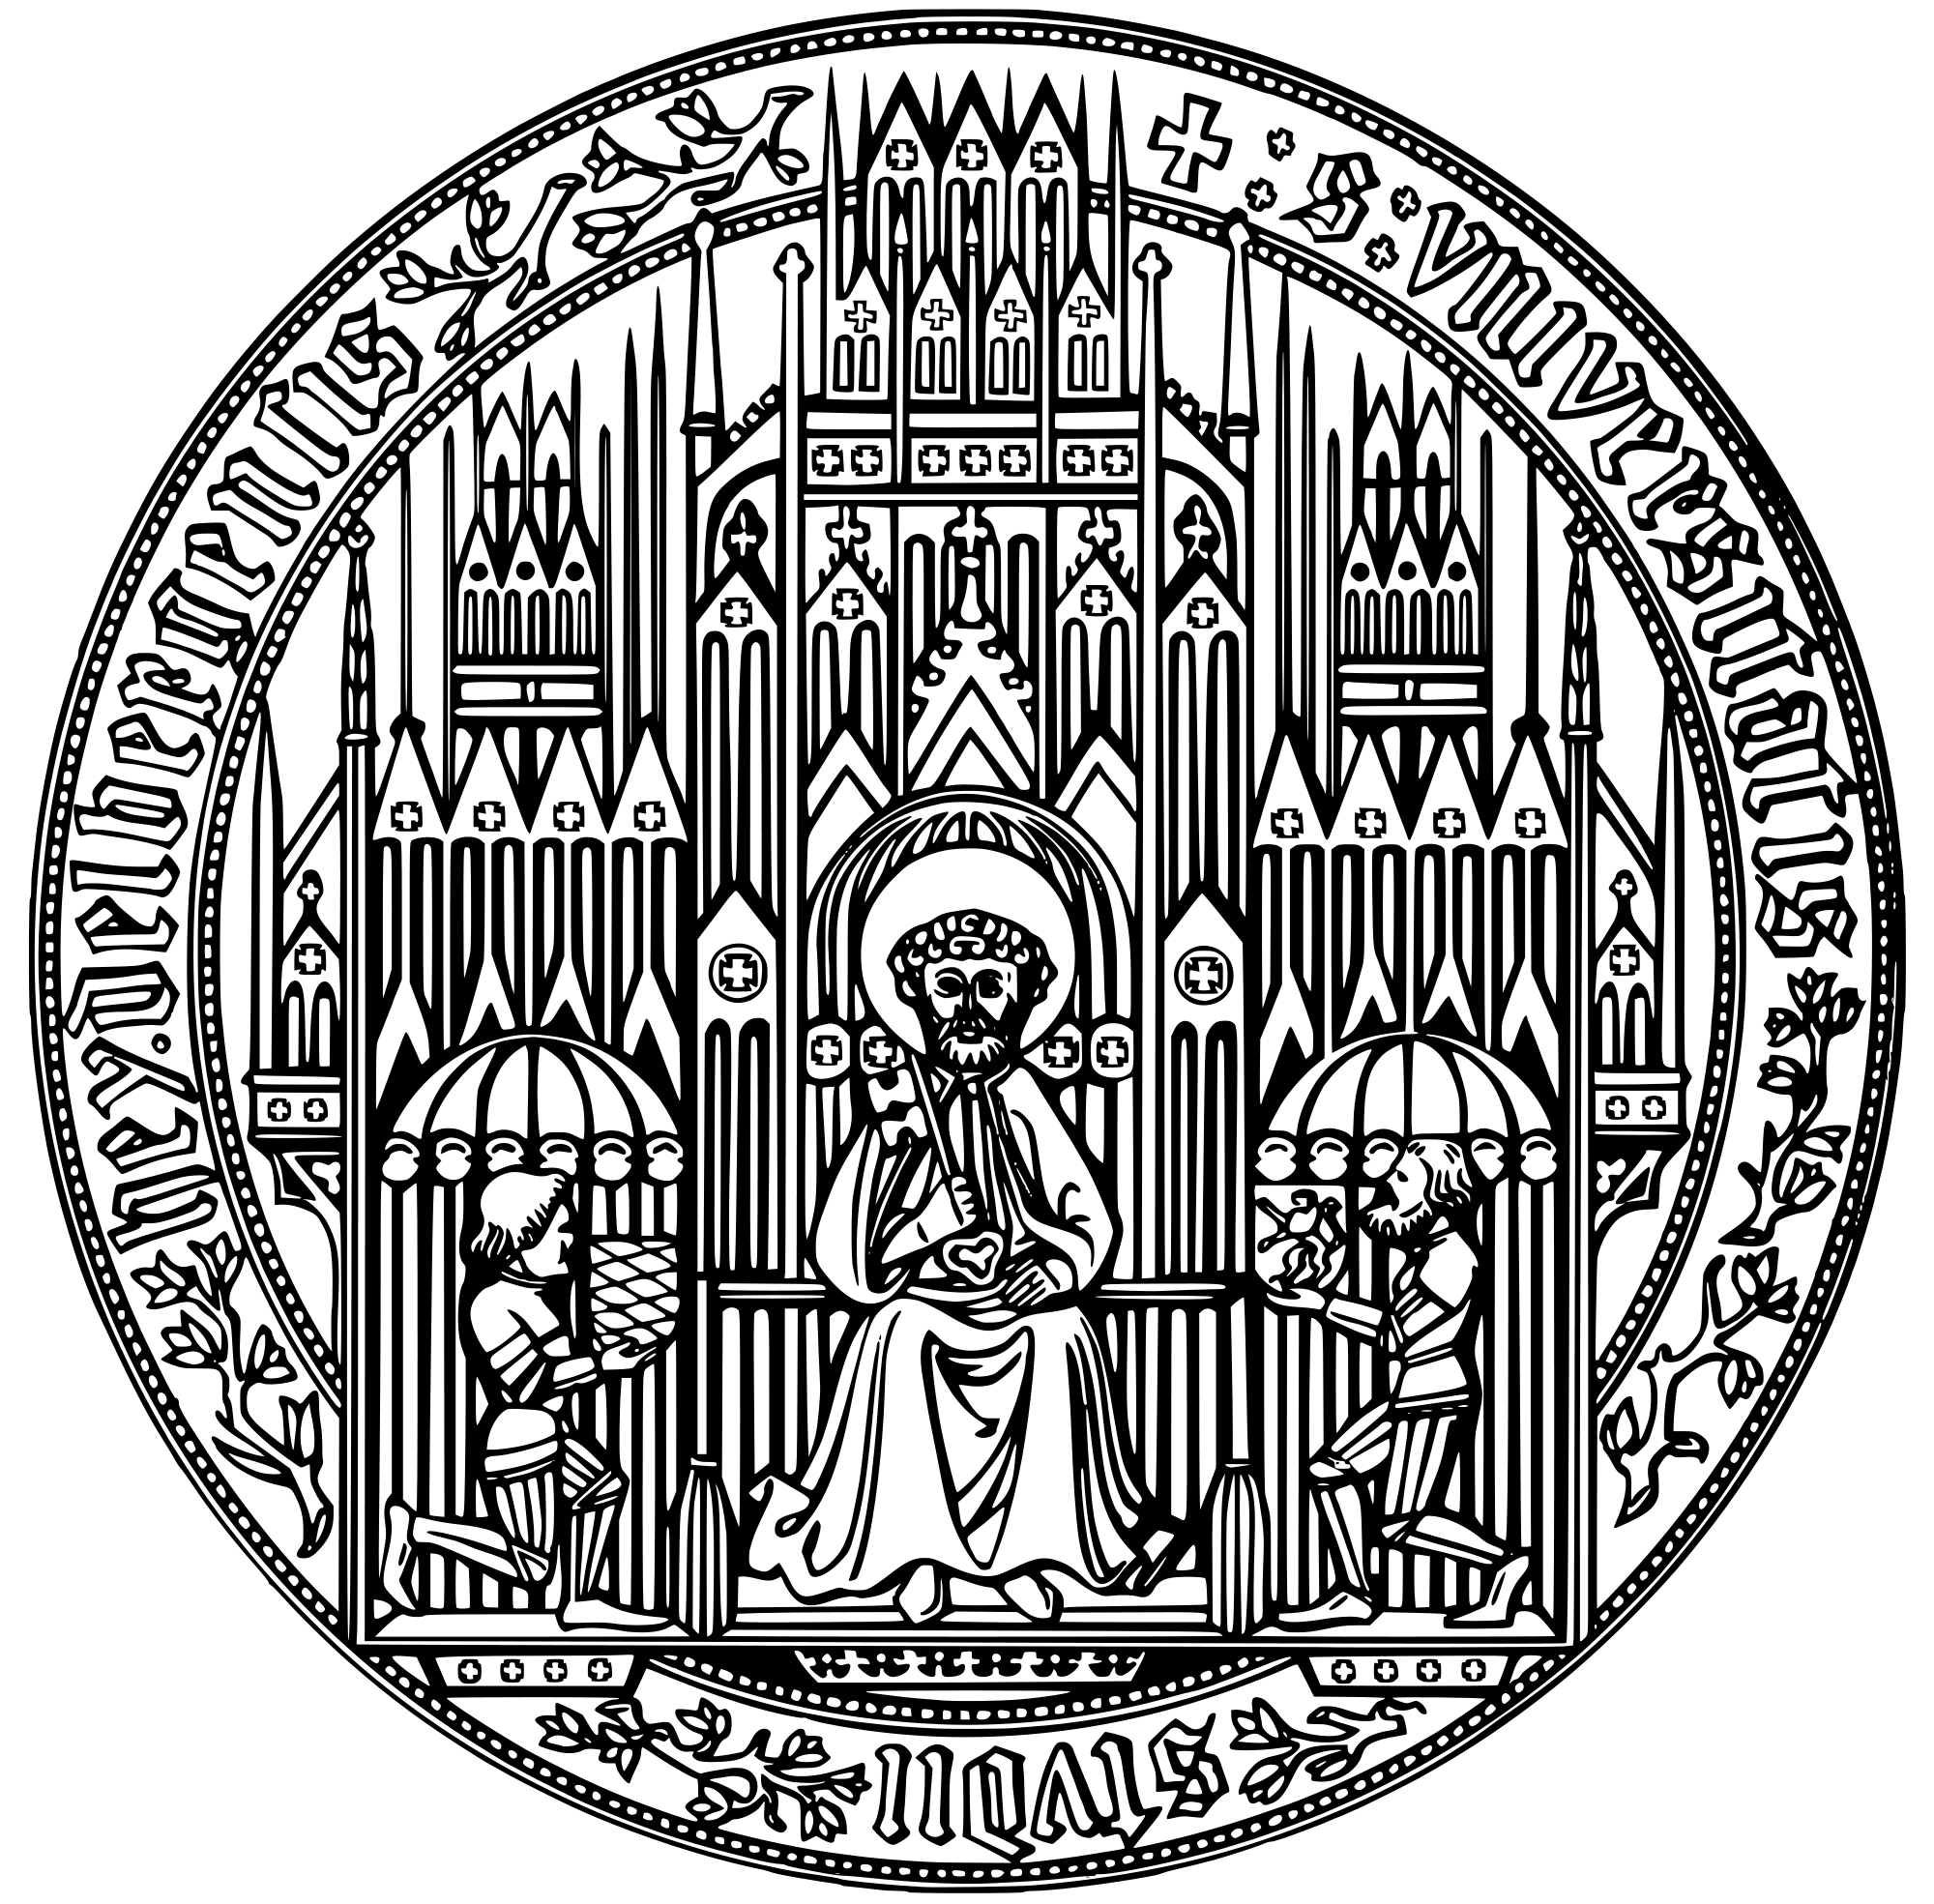
\includegraphics[width=0.08\textwidth]{Figures/Logos/logo_uhd}};
    \node[xshift=5.55cm, yshift=4.3cm] at (current page.center) {
\includegraphics[width=0.11\textwidth]{Figures/Logos/logo_emmy_noether_gross.jpg}};

    \end{tikzpicture}
\end{frame}

\begin{frame}{Motivation - Bachelor Thesis}
    \begin{tikzpicture}[remember picture,overlay]
    \node[xshift=-3.4cm, yshift=0.4cm] at (current page.center) {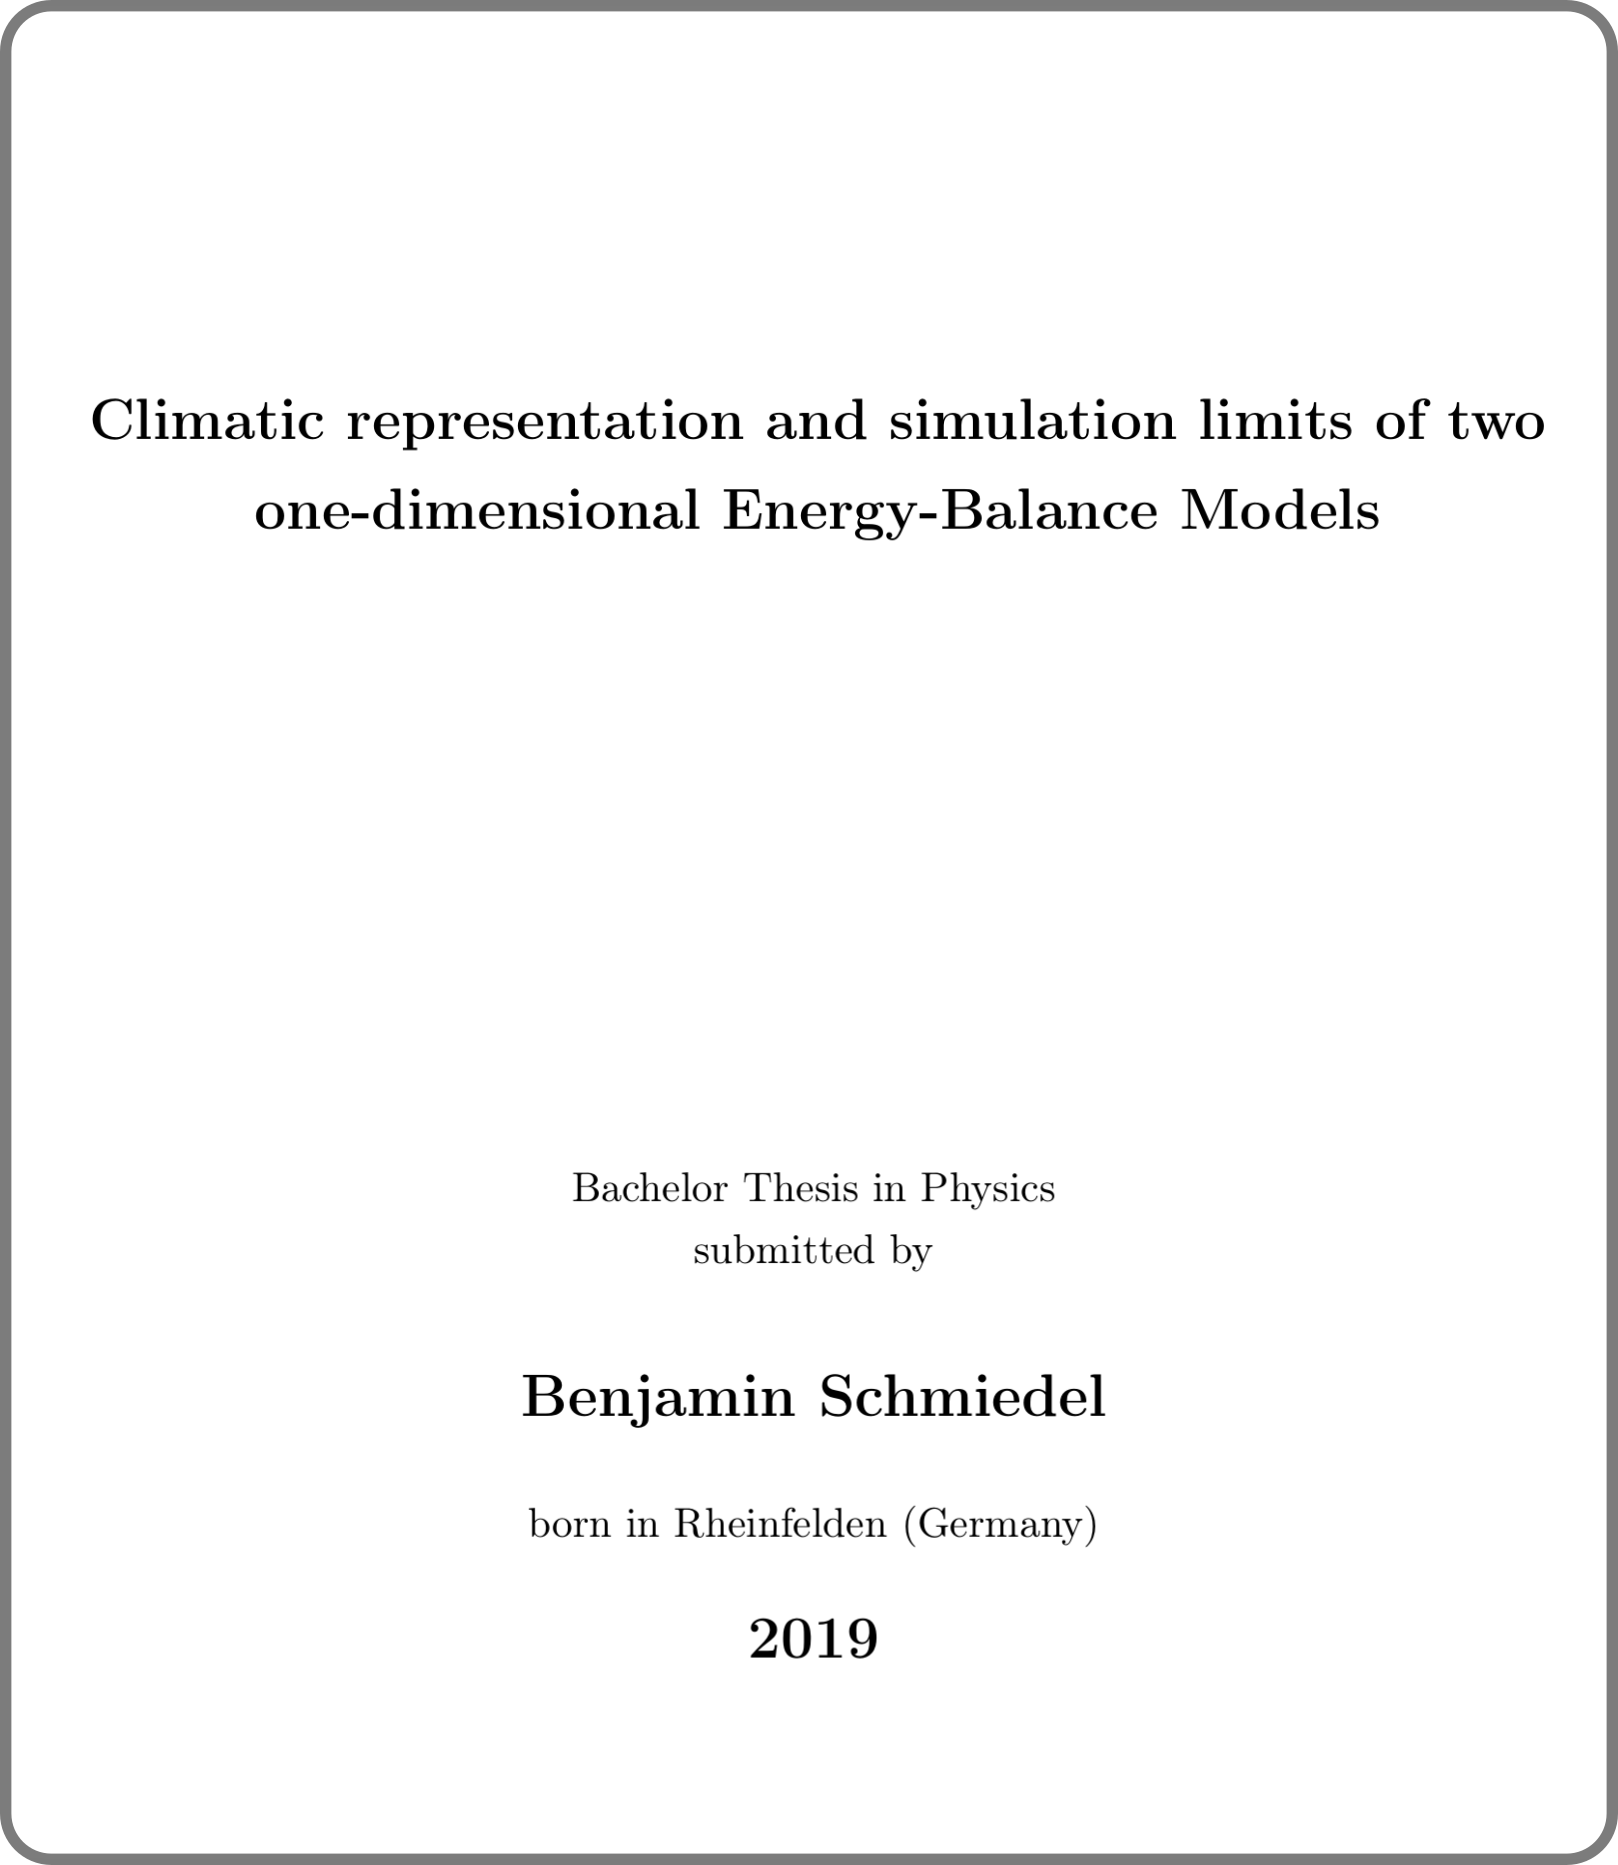
\includegraphics[width=0.5\textwidth]{Figures/Motivation/BT_Title_1.png}};
    \node[xshift=-4.2cm, yshift=-3.75cm] at (current page.center) {
\includegraphics[width=0.15\textwidth]{Figures/Logos/LogoIUP.png}};
    \node[xshift=-2.4cm, yshift=-3.75cm] at (current page.center) {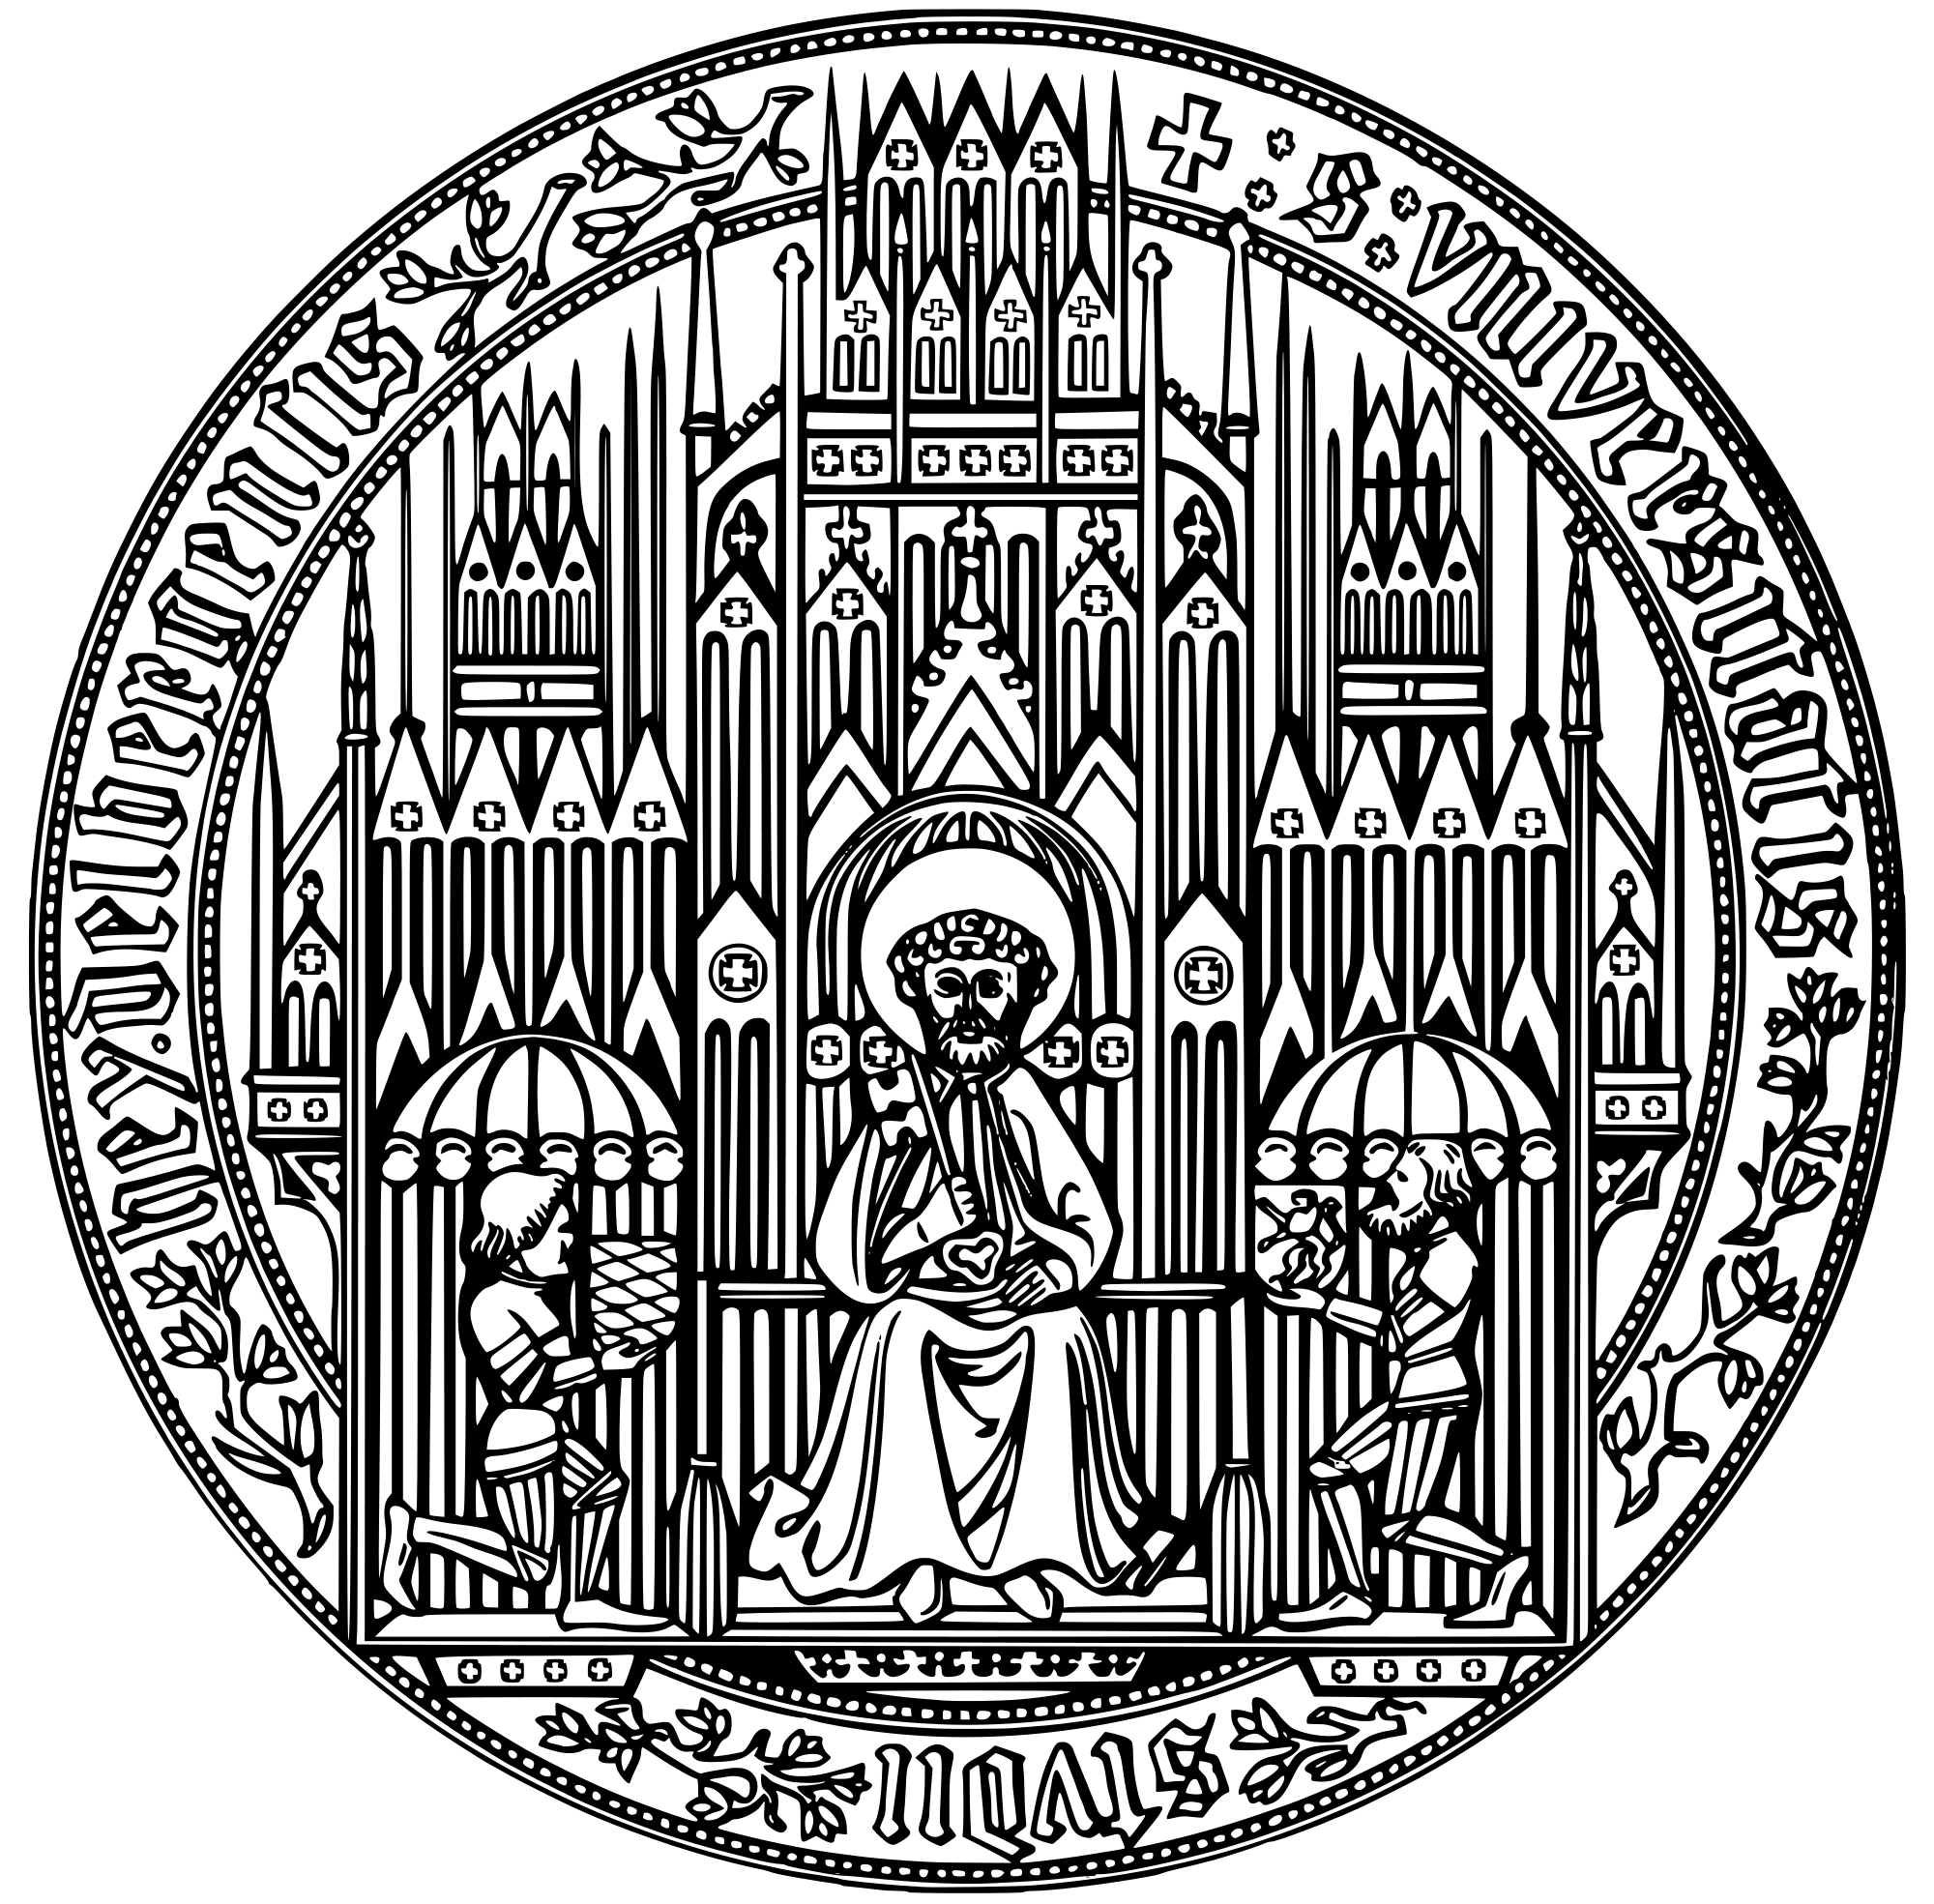
\includegraphics[width=0.15\textwidth]{Figures/Logos/logo_uhd}};
    \node[xshift=2.6cm, yshift=-1.85cm] at (current page.center) {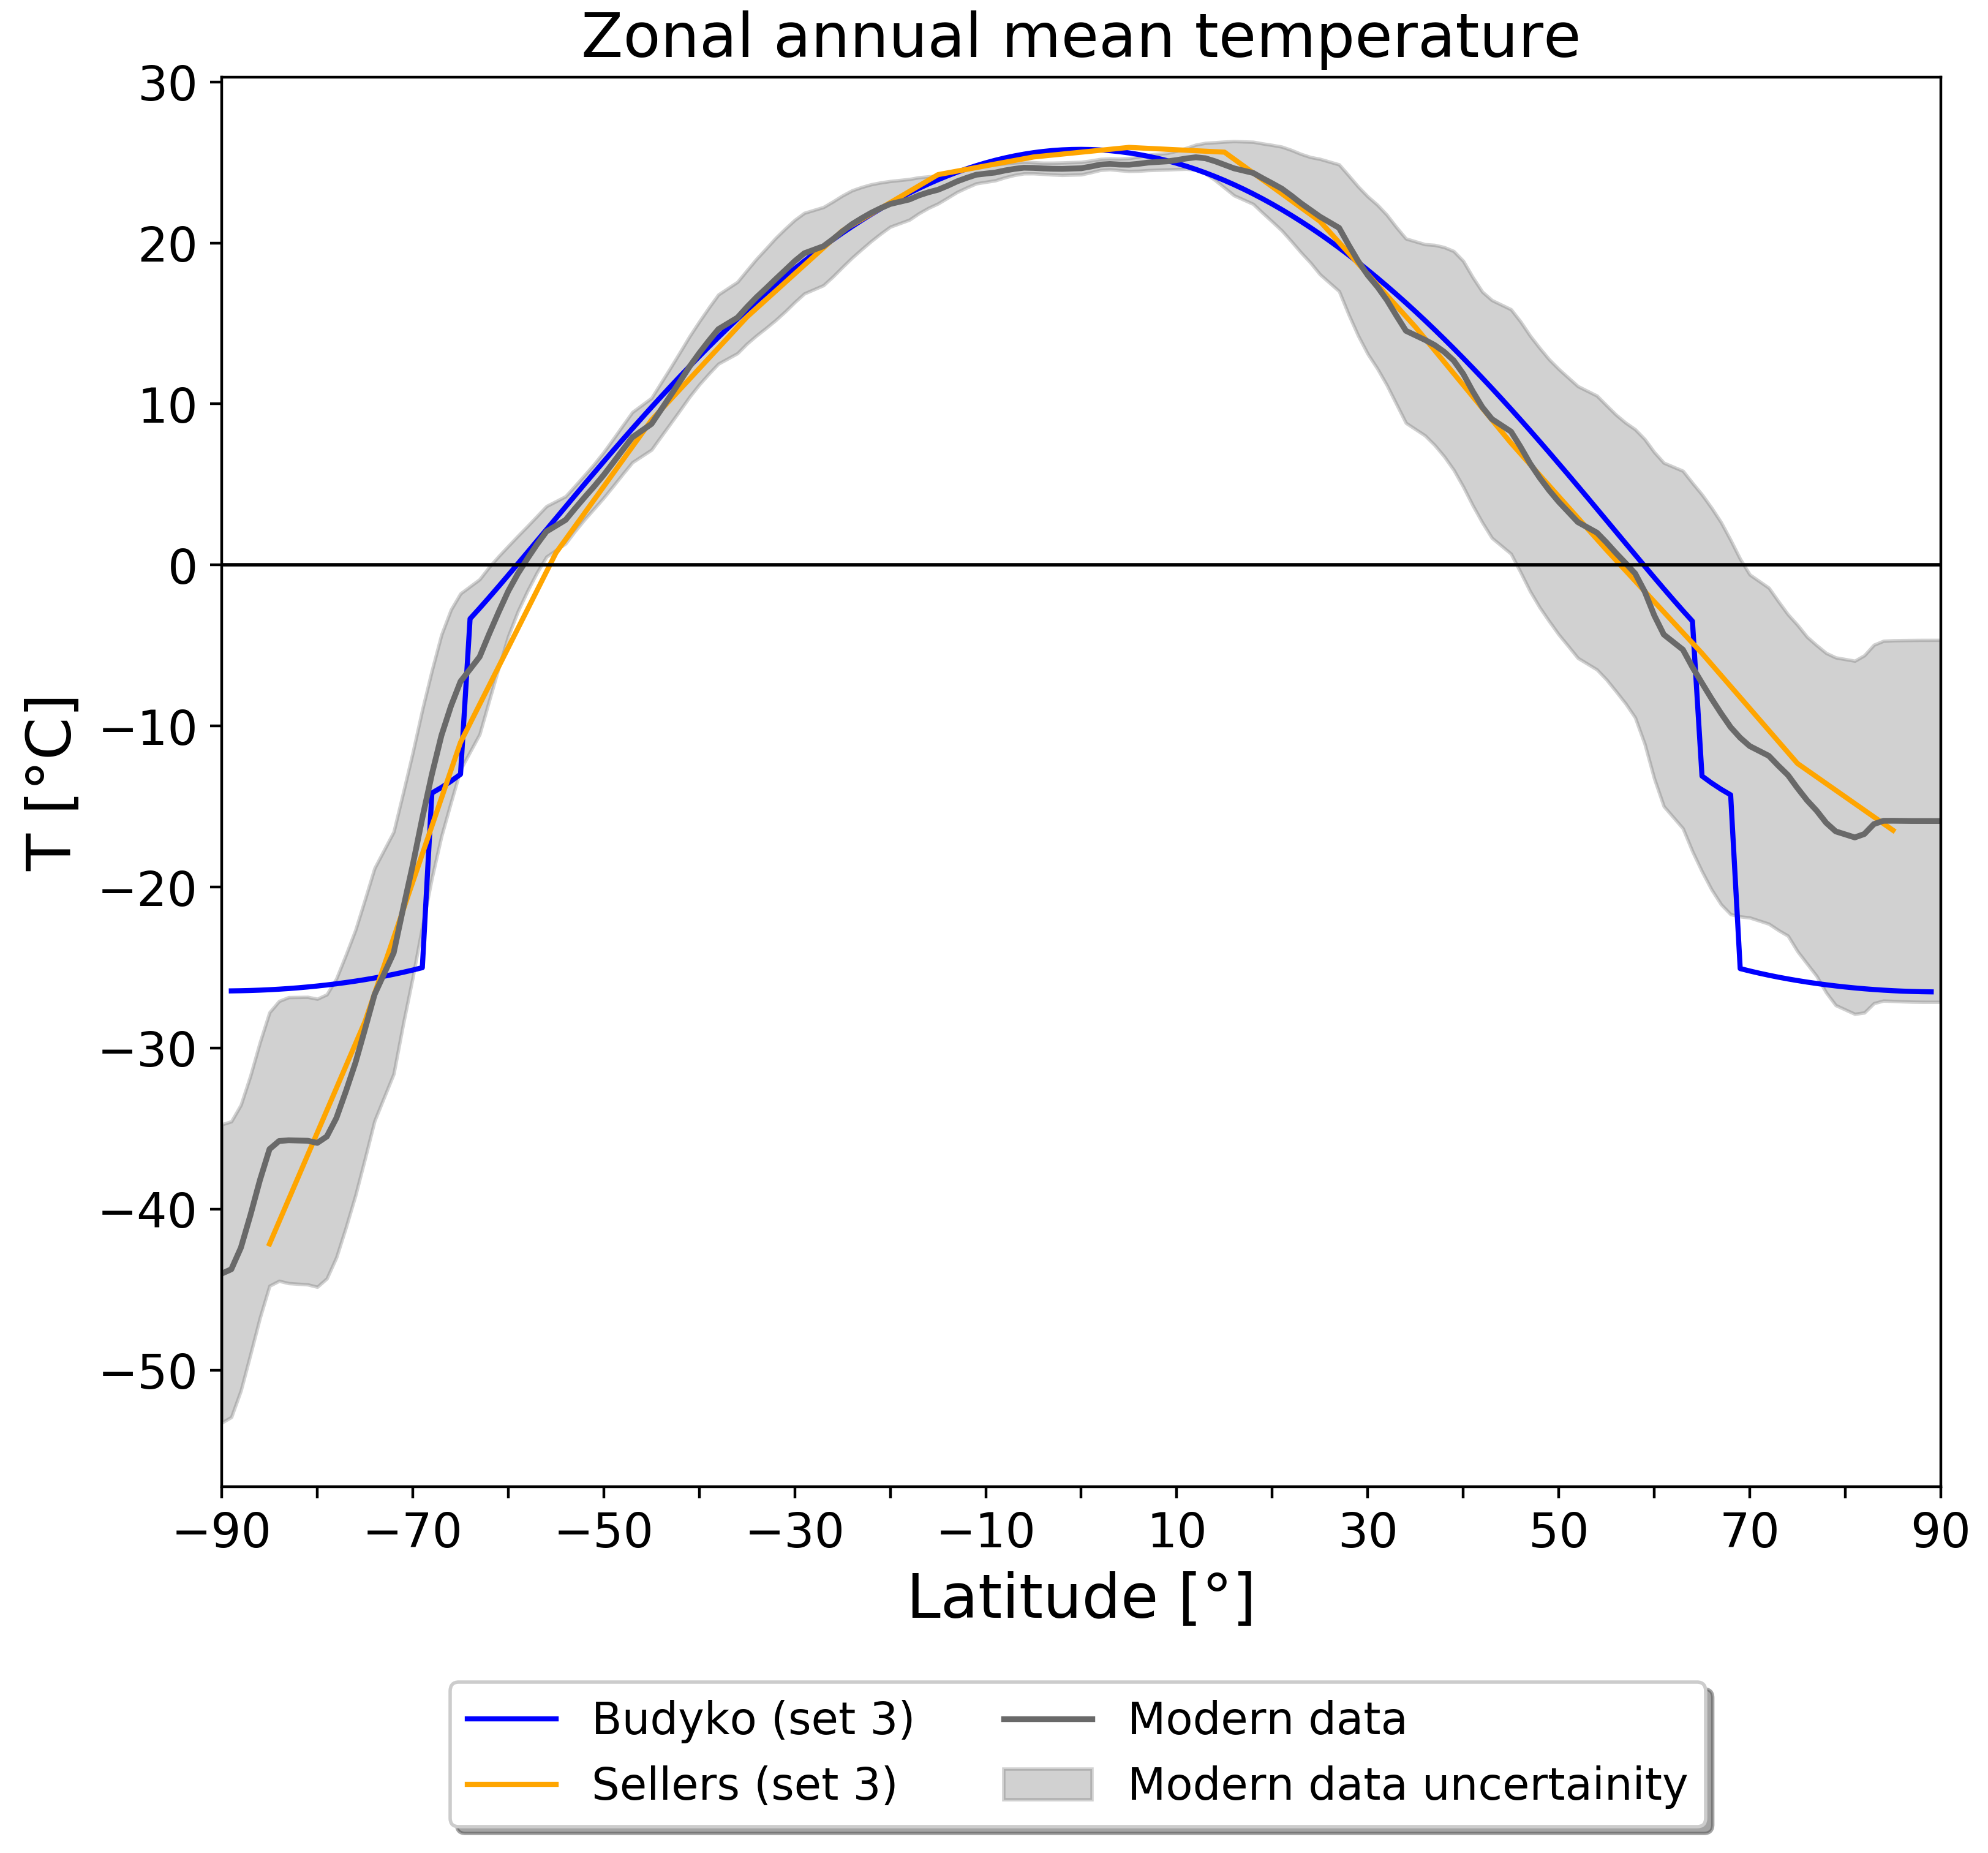
\includegraphics[width=0.55\textwidth]{Figures/Motivation/BT_Validation.png}};
    \node[xshift=1.8cm, yshift=2.25cm] at (current page.center) {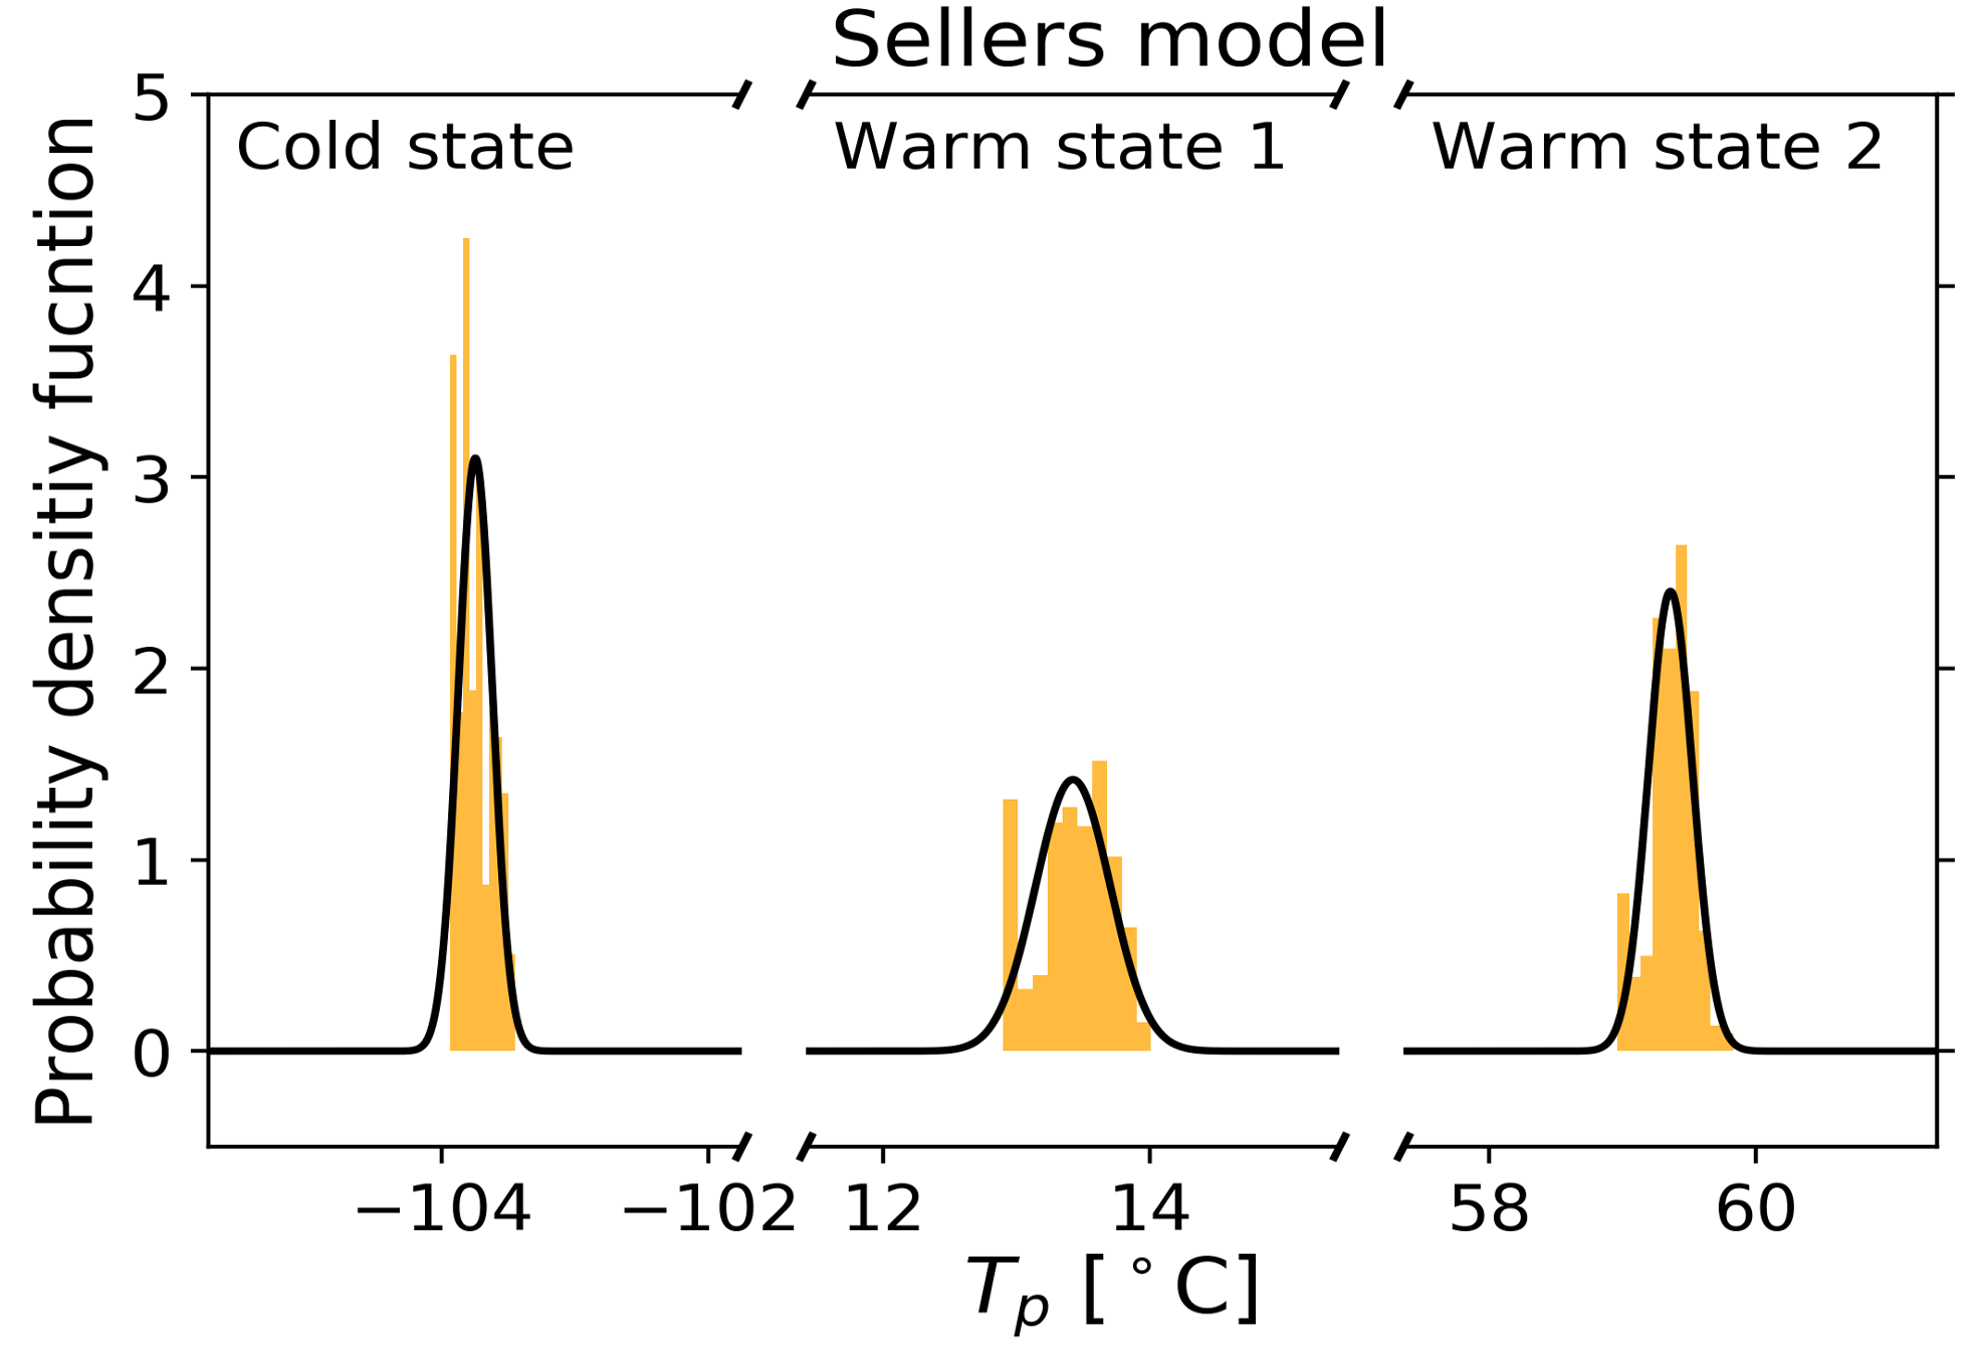
\includegraphics[width=0.35\textwidth]{Figures/Motivation/BT_Variability_Cut.png}};
    \end{tikzpicture}
\end{frame}

\begin{frame}{Motivation - Development}
    \begin{tikzpicture}[remember picture,overlay]
    \node[xshift=-0cm, yshift=0cm] at (current page.center) {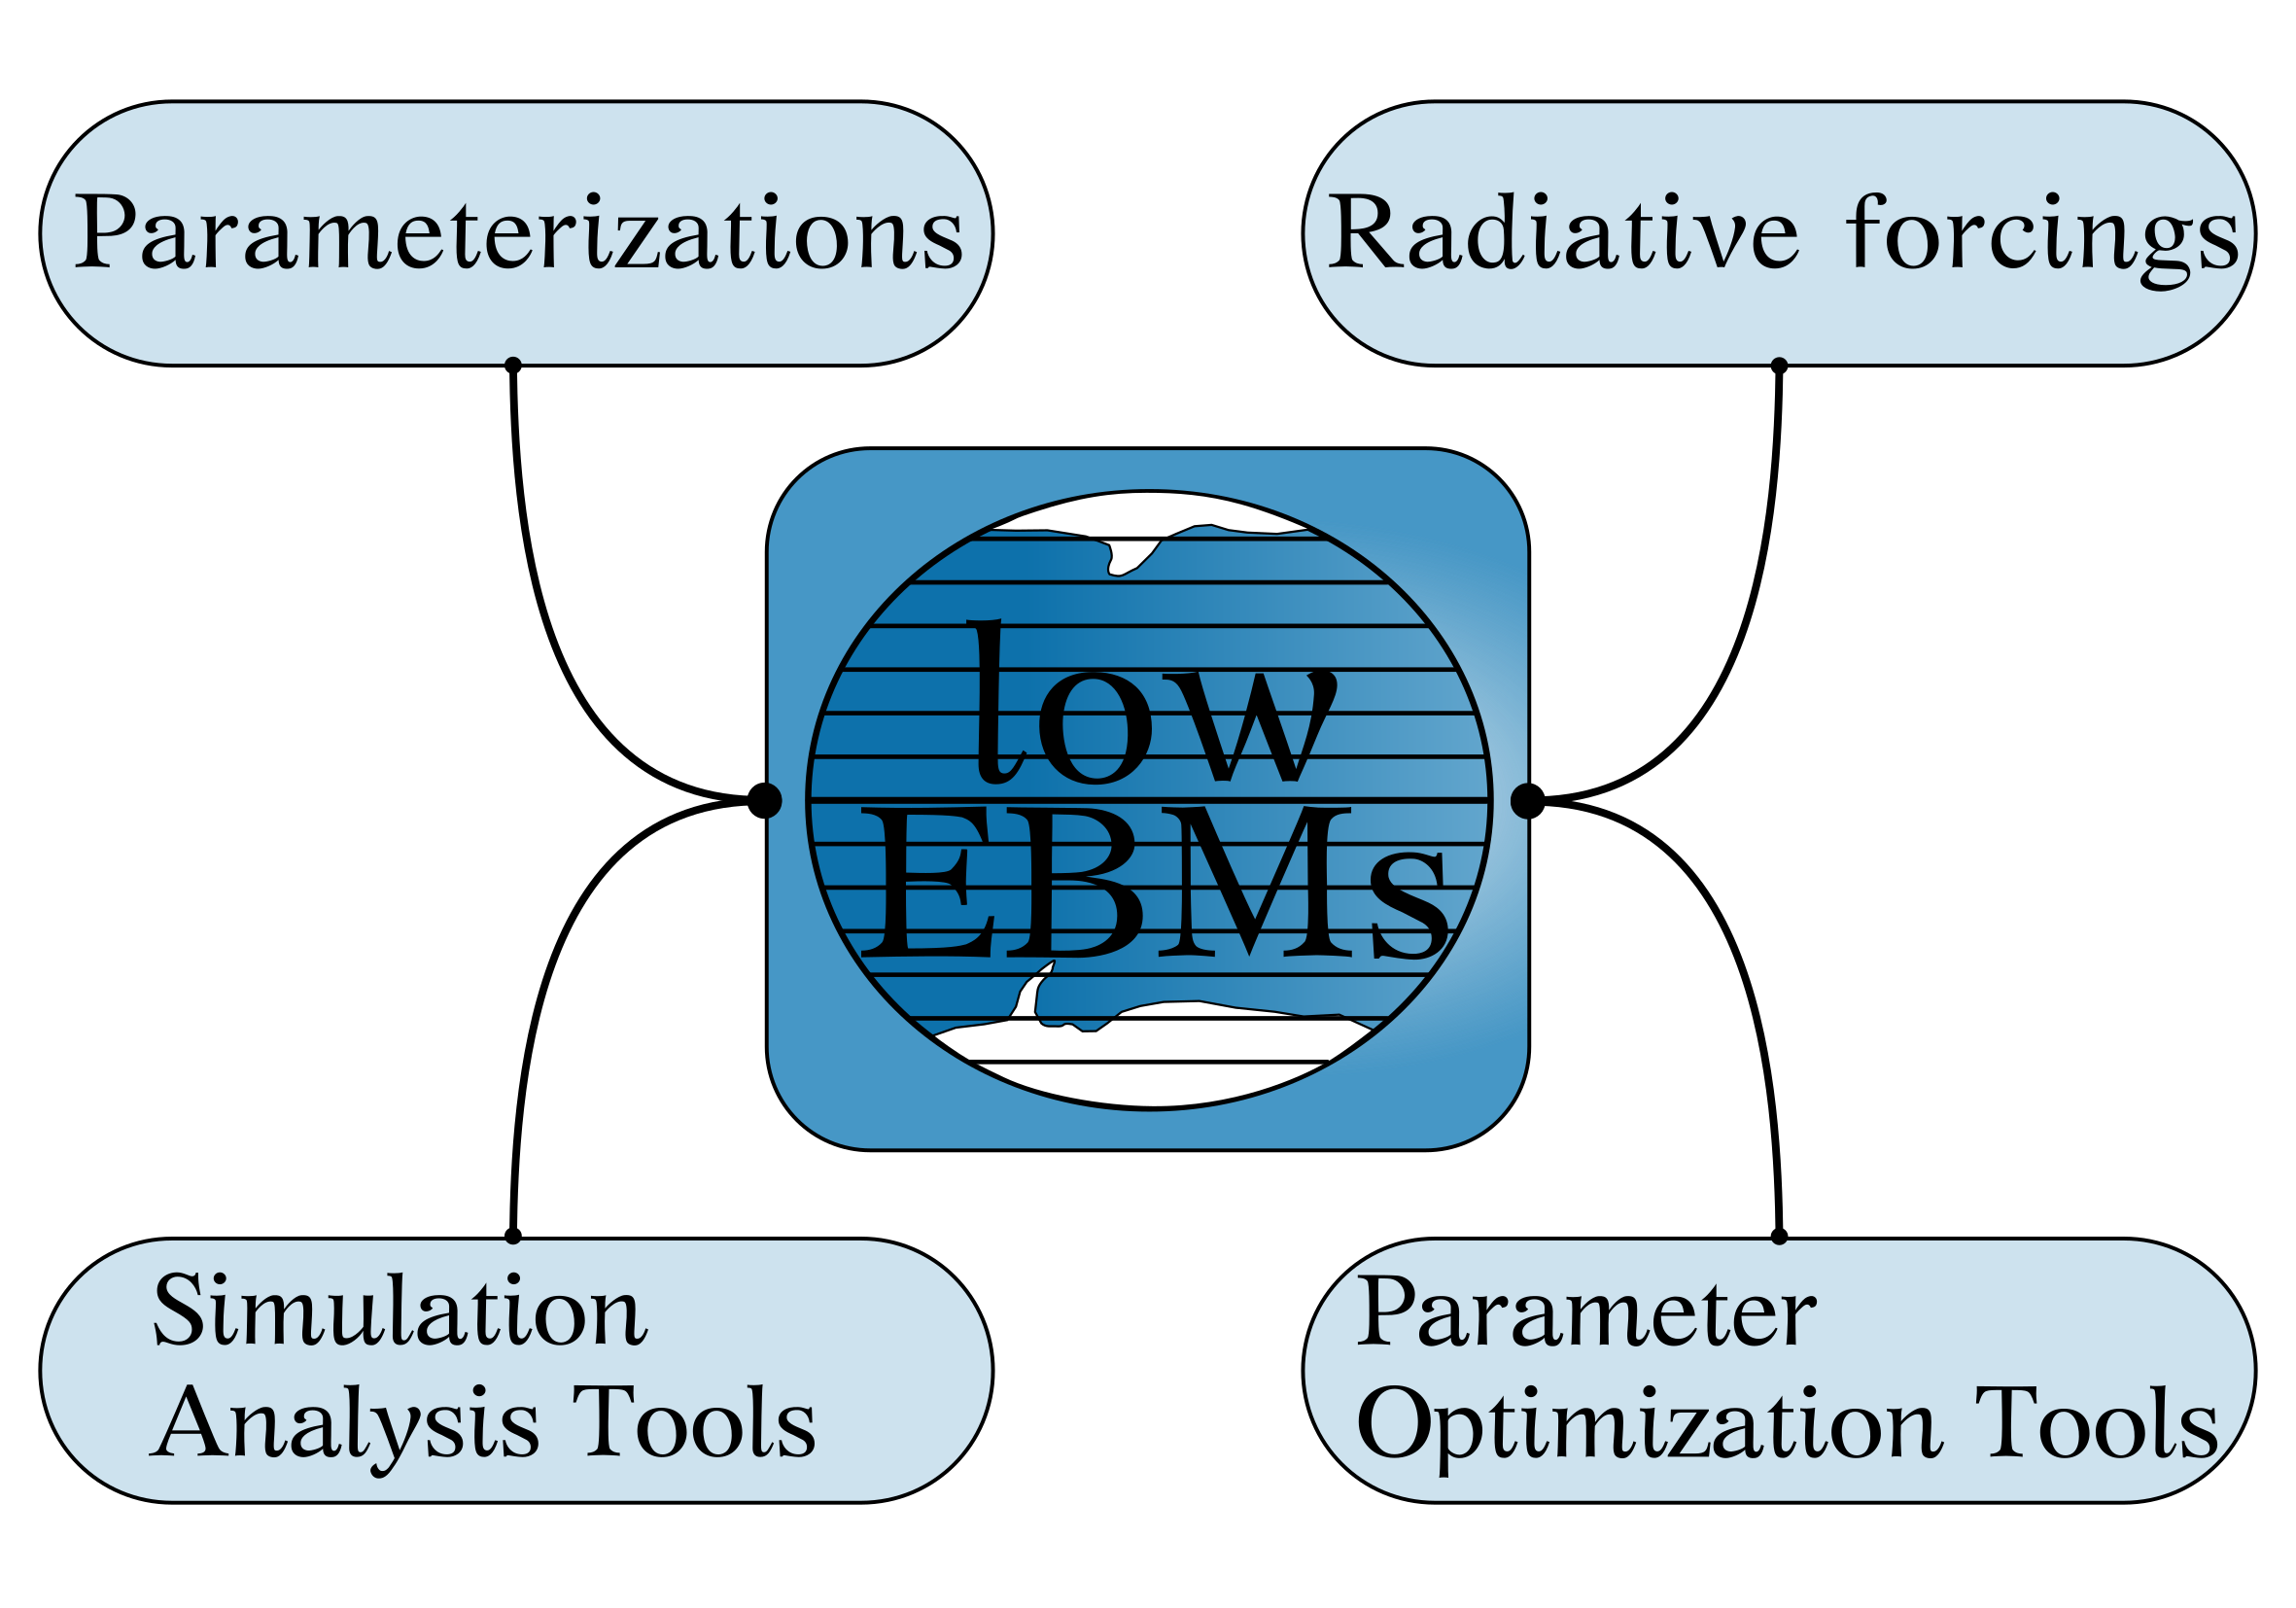
\includegraphics[width=\textwidth]{Figures/Motivation/Content_Map.png}};
    \node[xshift=3.6cm, yshift=4.3cm] at (current page.center) {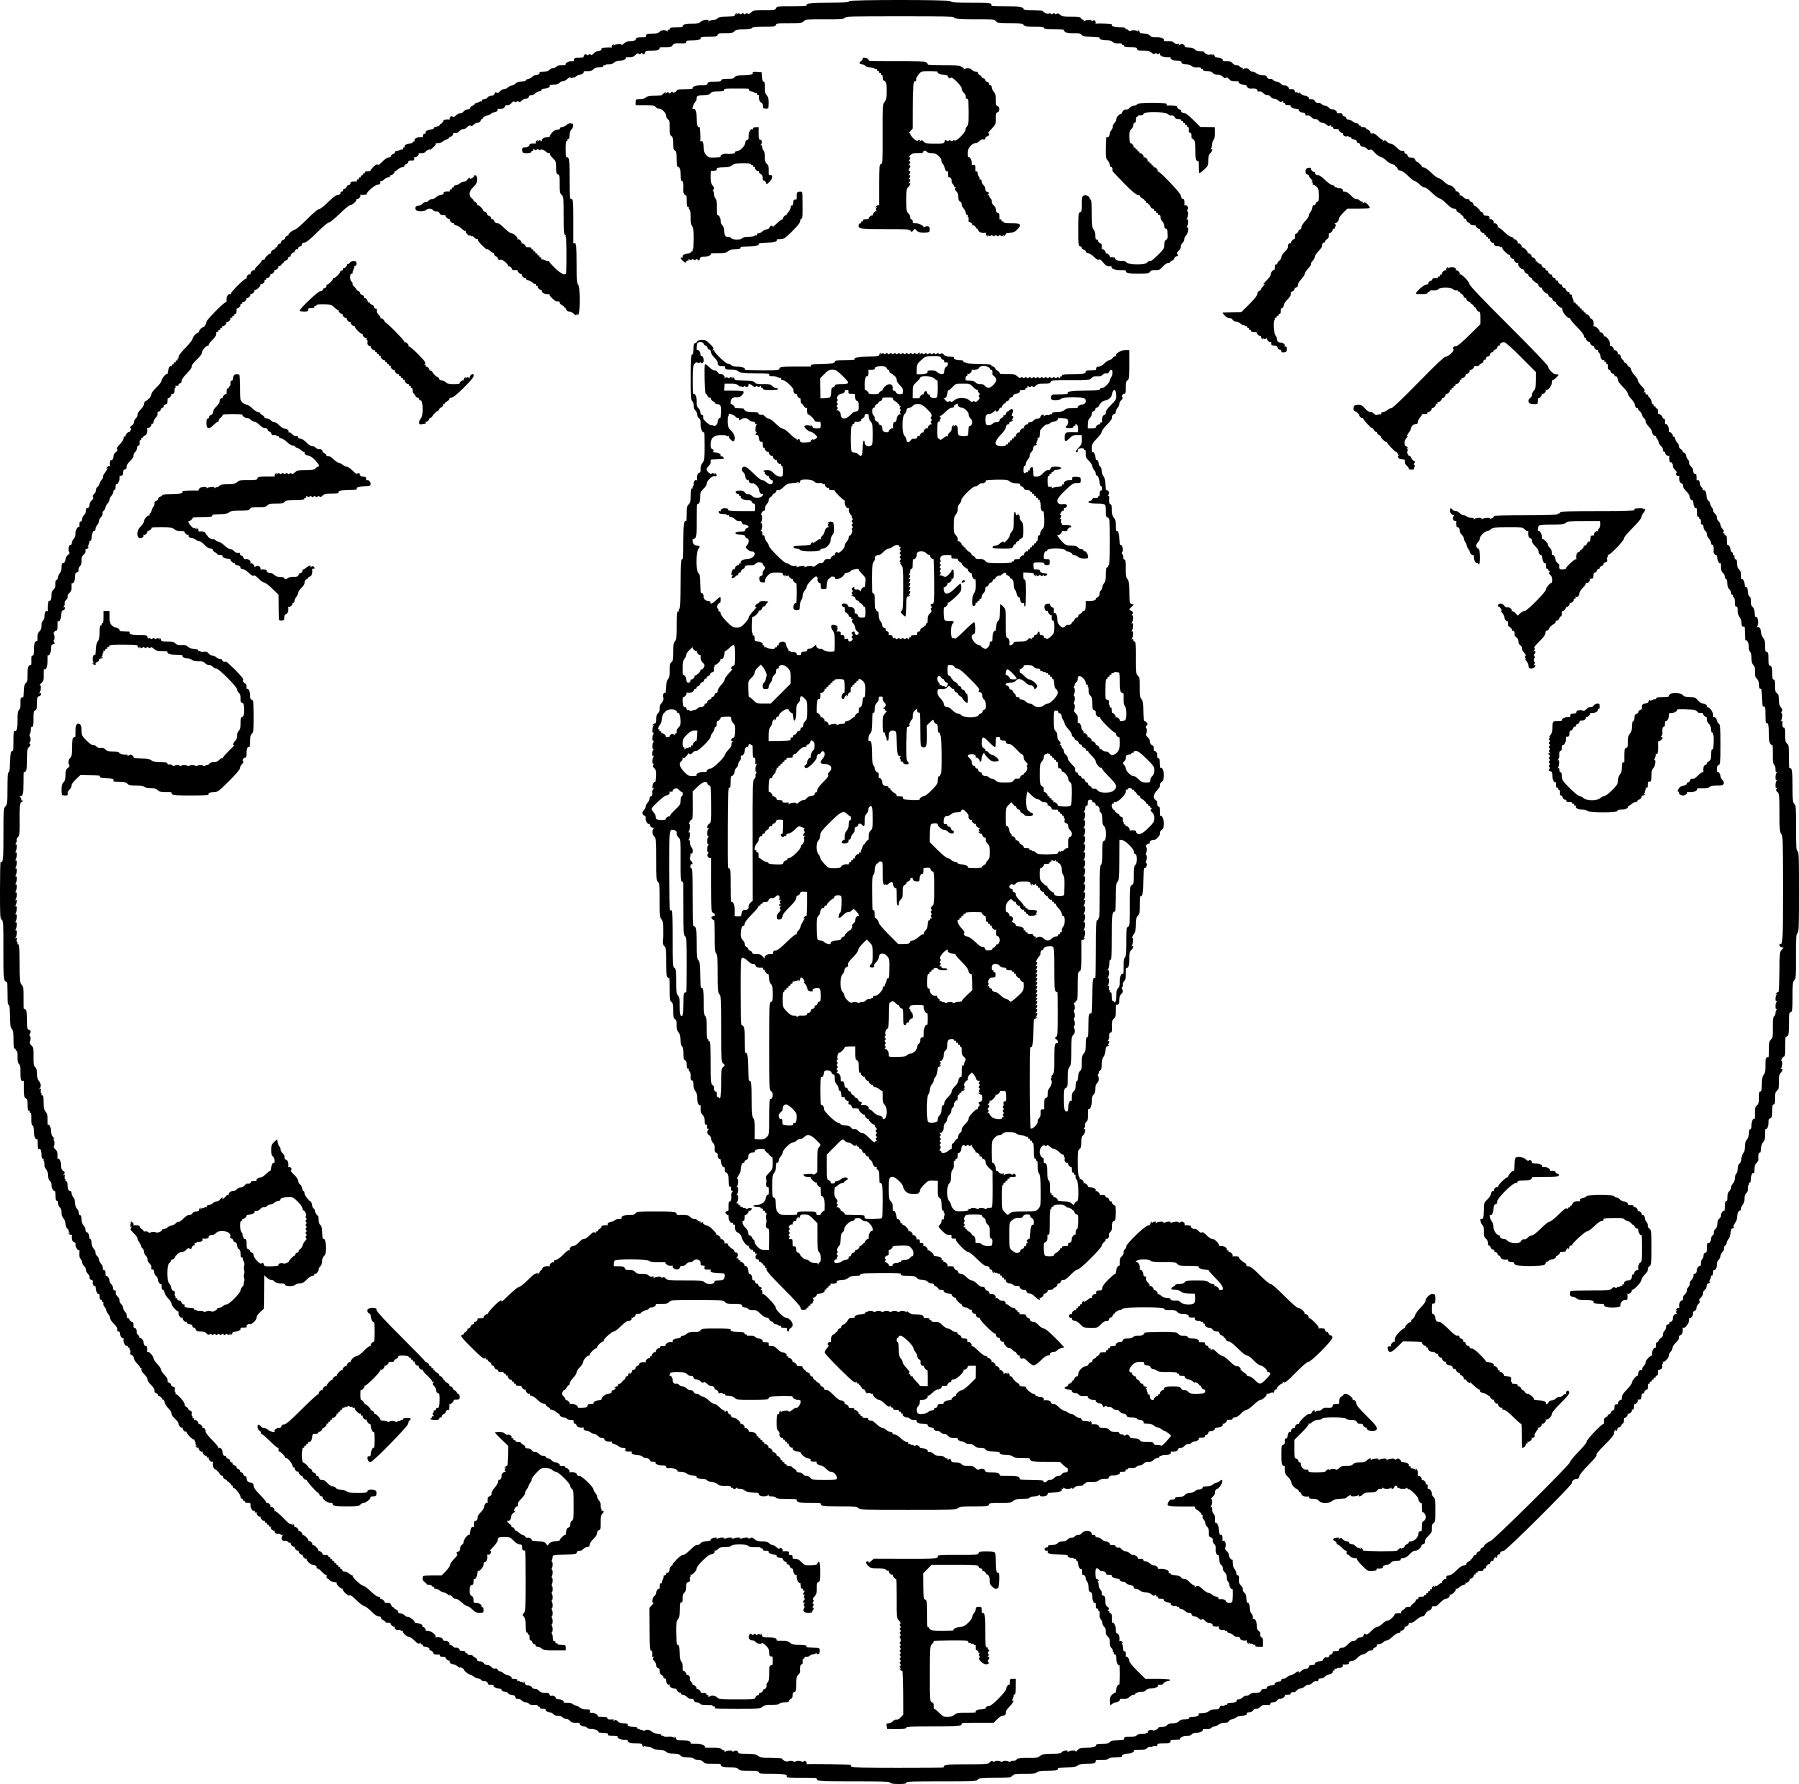
\includegraphics[width=0.08\textwidth]{Figures/Logos/logo_bergen.png}};
    \node[xshift=5.25cm, yshift=4.3cm] at (current page.center) {
\includegraphics[width=0.19\textwidth]{Figures/Logos/bjerkneslogo_big.png}};

    \end{tikzpicture}
\end{frame}

\begin{comment}
\begin{frame}{Table of Content}
    \begin{itemize}
        \item Motivation
        \item Theoretical Background
        \item Implementation details
        \item Application period
        \item Practical demonstration [Run in Jupyter on different screen] 
        \item Additional features
        \item Outlook
    \end{itemize}
\end{frame}
\end{comment}

\setbeamerfont{section number projected}{%
  family=\rmfamily,series=\bfseries,size=\normalsize}
\setbeamercolor{section number projected}{bg=darkred,fg=white}
\setbeamertemplate{section in toc}[ball]

\begin{frame}{Table of Content}
	\tableofcontents
\end{frame}	
	
\begin{comment}
\begin{frame}{Theoretical Background}
    \begin{itemize}
        \item Energybalance (IPCC), Step of simplification (graphical)
        \item Terms which are featured, 0D / 1D
        \item Model equation
        \item Parameterizations (as map?)
    \end{itemize}
\end{frame}
\end{comment}

\section{Theoretical Background}

\begin{frame}{Theoretical background - Energy balance}
    \begin{tikzpicture}[remember picture,overlay]
    \node[xshift=-0cm, yshift=0cm] at (current page.center) {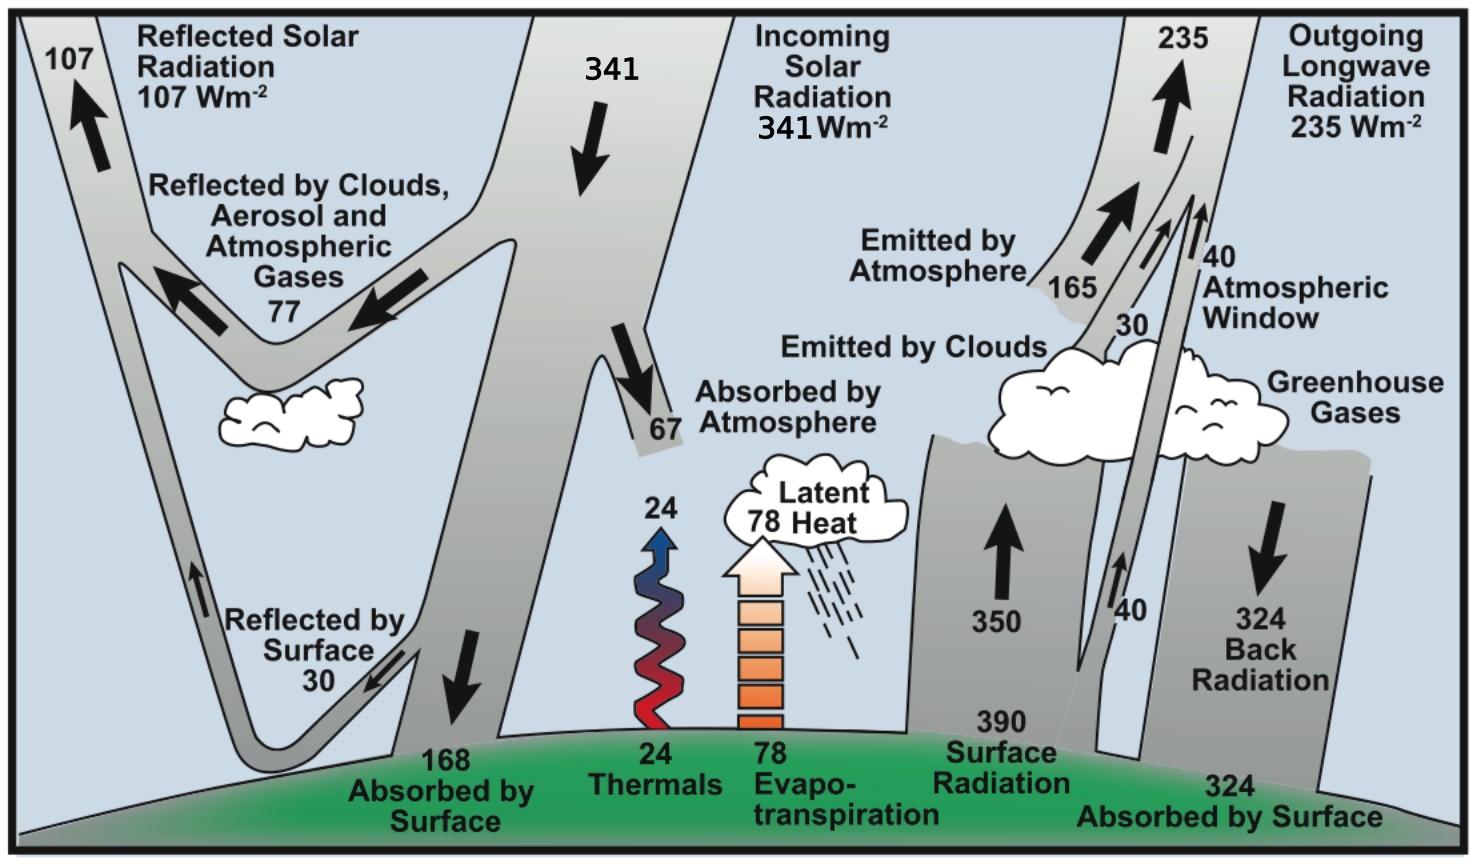
\includegraphics[width=\textwidth]{Figures/Background/EB.png}};
    \end{tikzpicture}
    \blfootnote{[Kiehl and Trenberth 1997]}
\end{frame}

\begin{frame}{Theoretical background - Energy balance}
    \begin{tikzpicture}[remember picture,overlay]
    \node[xshift=-0cm, yshift=0cm] at (current page.center) {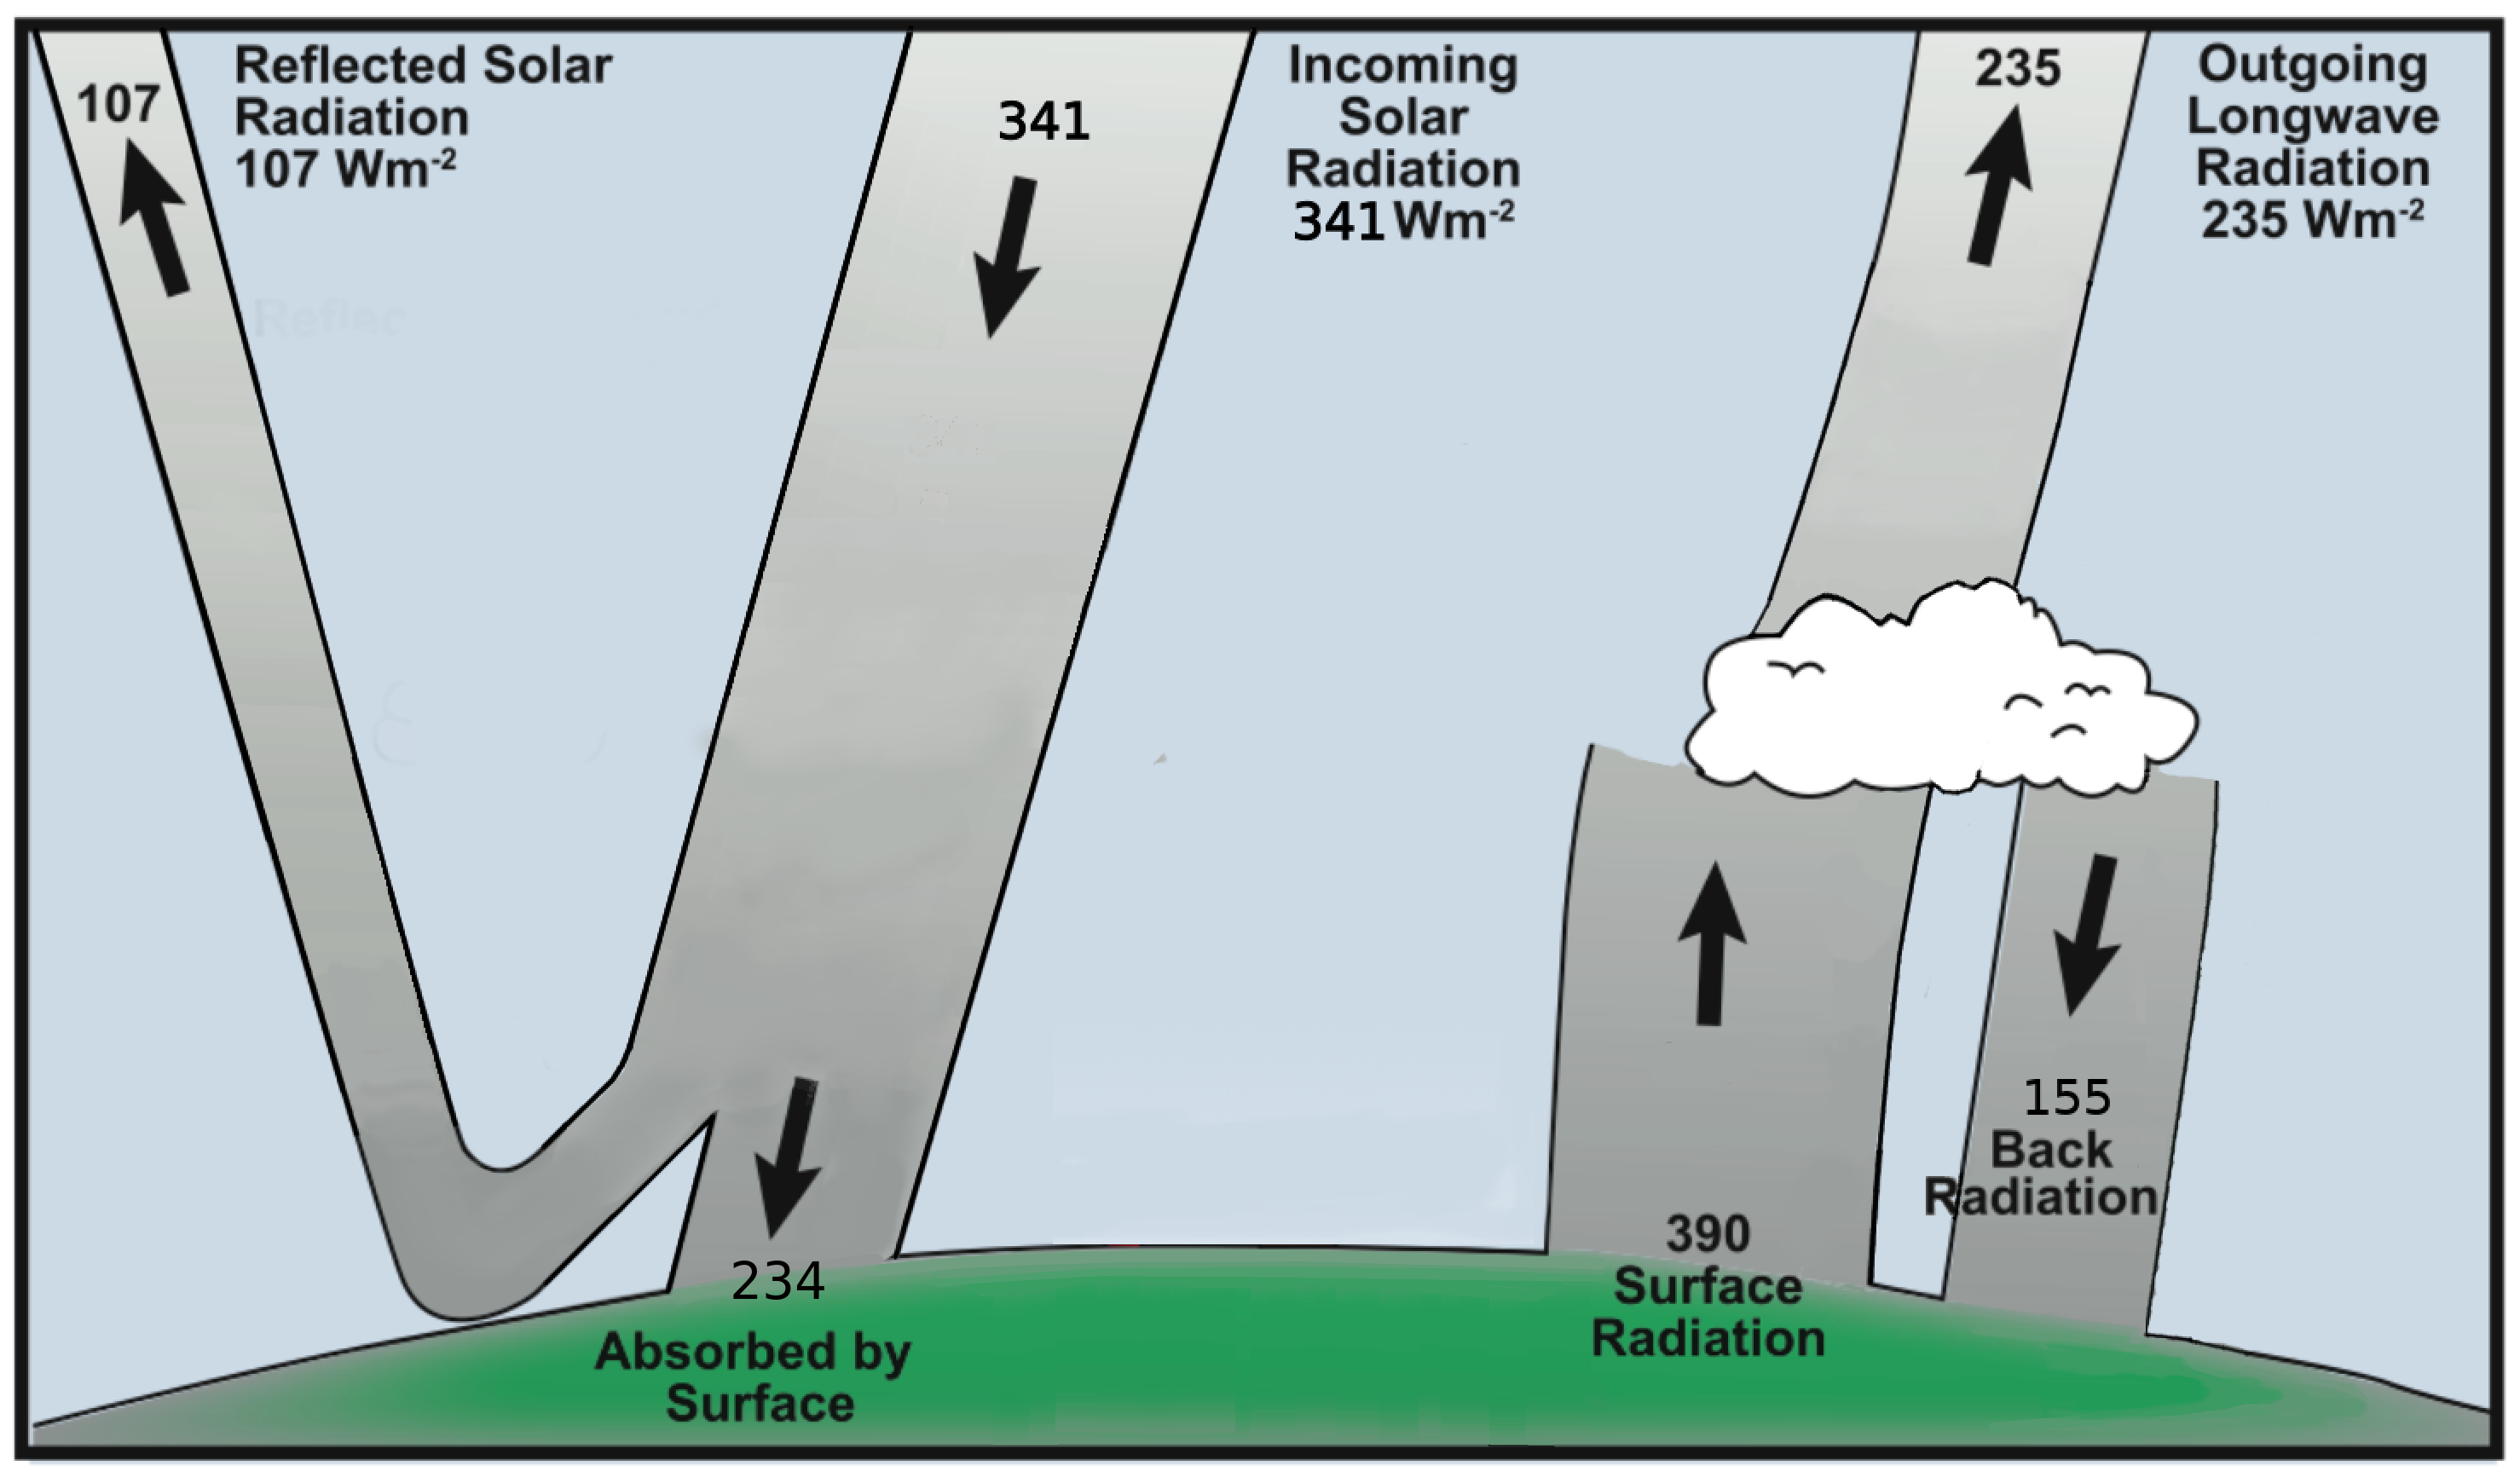
\includegraphics[width=\textwidth]{Figures/Background/EB_reduced.png}};
    \onslide<2>{\node[xshift=-0cm, yshift=0cm] at (current page.center){
	\mybox{
	\begin{align*}
	C \frac{dT}{dt} = R_{\downarrow}  - R_{\uparrow}\\
	\end{align*}}};}
    \end{tikzpicture}
    \blfootnote{[Kiehl and Trenberth 1997, modified]}
\end{frame}

\begin{frame}{Theoretical background - Dimension of realization}
    \begin{tikzpicture}[remember picture,overlay]
    \node[xshift=-3cm,yshift=1.6cm] at (current page.center) {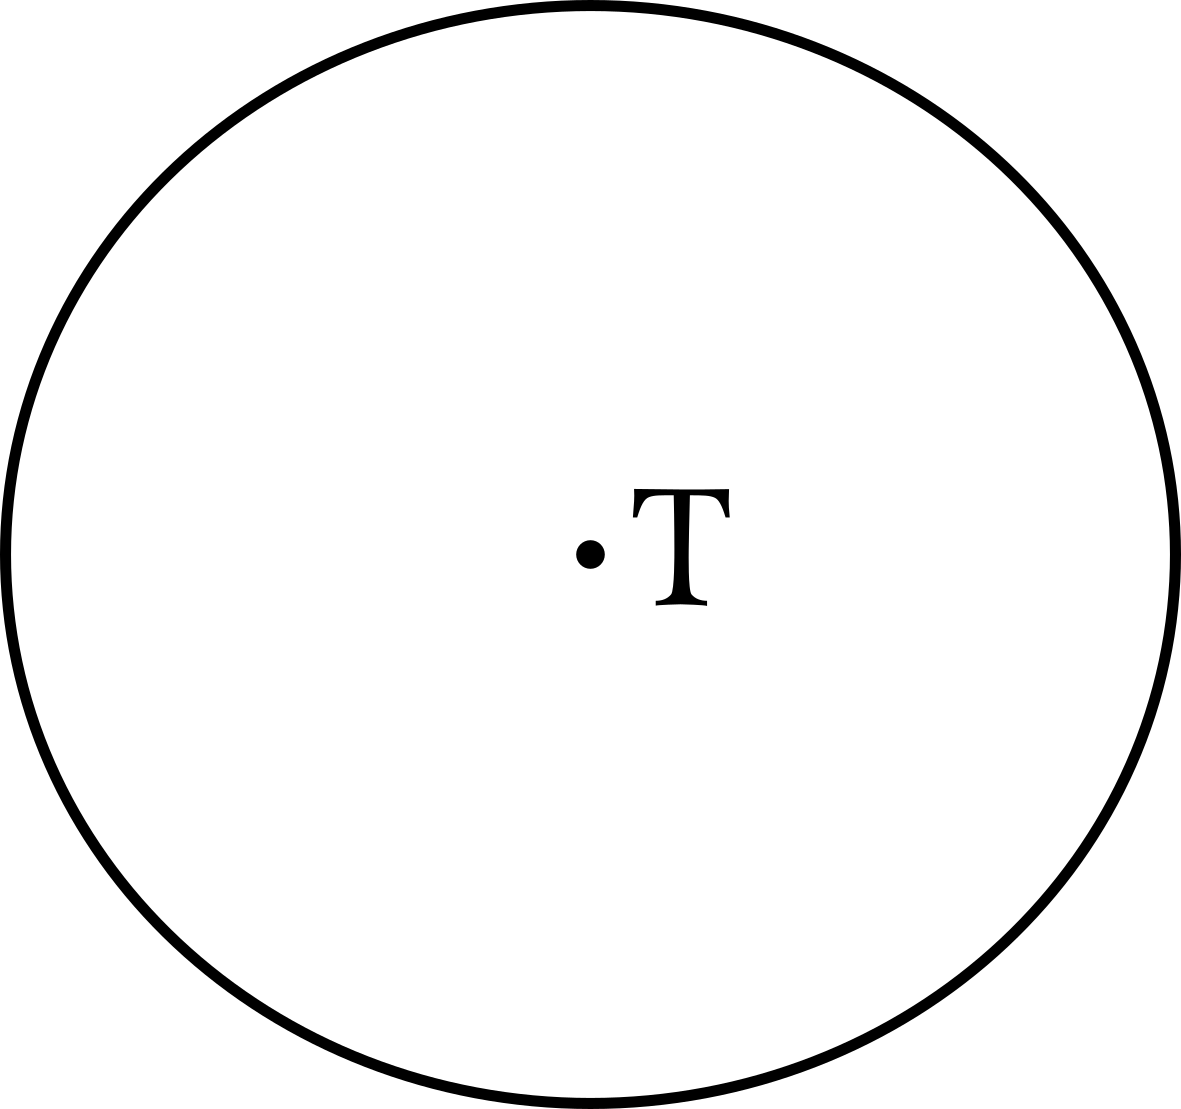
\includegraphics[width=0.35\textwidth]{Figures/Background/Grid0D.png}
	};
	\node[xshift=-3cm,yshift=-2.2cm] at (current page.center) {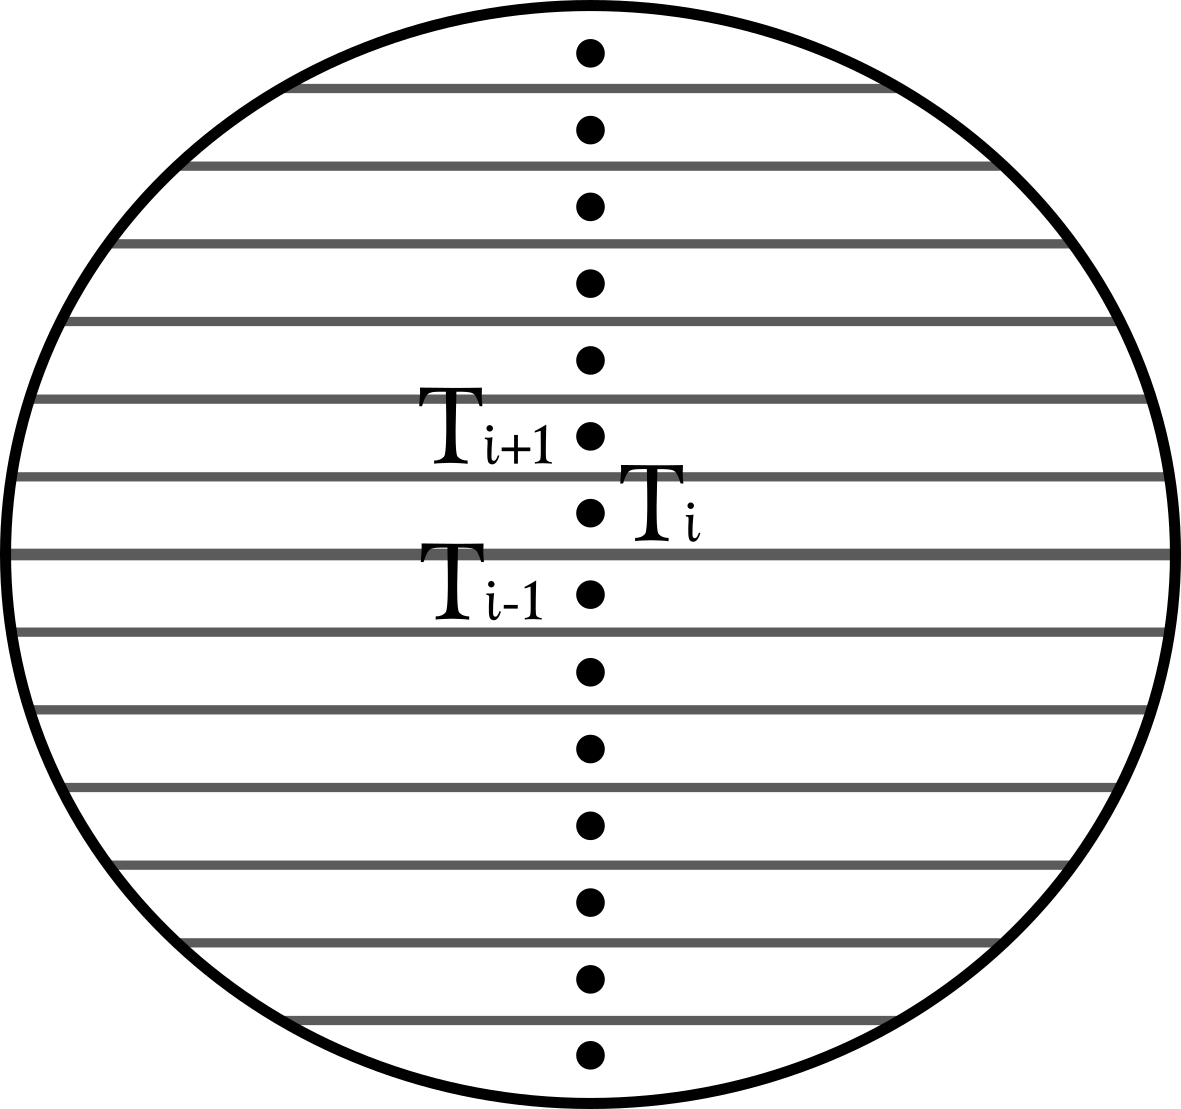
\includegraphics[width=0.35\textwidth]{Figures/Background/Grid1D.png}
	};
	\node[align=left,xshift=2cm,yshift=2.6cm] at (current page.center) {\underline{Zero dimensional}};
    \node[xshift=2cm,yshift=1.6cm] at (current page.center) {
            $\begin{aligned}
            C \frac{dT}{dt} = R_{\downarrow}  - R_{\uparrow}
            \end{aligned}$
	};
	\node[align=left,xshift=2cm,yshift=-1.2cm] at (current page.center) {\underline{One dimensional}};
	\node[xshift=2cm,yshift=-2.2cm] at (current page.center) {
            $\begin{aligned}
            C \frac{dT_i}{dt} = R_{\downarrow,i}  - R_{\uparrow,i}
            \end{aligned}$
	};
    \end{tikzpicture}
\end{frame}

\begin{frame}{Theoretical Background - Latitudinal Transfer}
    \begin{tikzpicture}[remember picture,overlay]
    \node[xshift=0cm,yshift=1cm] at (current page.center) {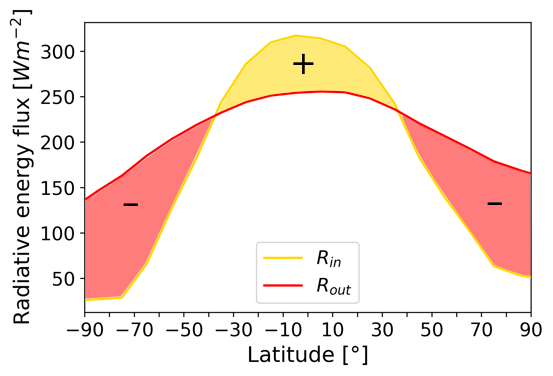
\includegraphics[width=0.6\textwidth]{Figures/Background/FluxDifference.png}
	};
    \node[xshift=0cm,yshift=-2.5cm] at (current page.center) {
    \mybox{
	\begin{align*}
    C \frac{dT_i}{dt} = R_{\downarrow,i}  - R_{\uparrow,i} +F_{transfer,i}\\
    \end{align*}}
	};
    \end{tikzpicture}
\end{frame}

\begin{frame}{Theoretical Background - Parameterizations}
    \begin{tikzpicture}[remember picture,overlay]
    \node[draw,xshift=-4.5cm,yshift=2.6cm] at (current page.center) {\Large{$R_{\downarrow}$}};
    \node[align=left,anchor=west,xshift=-3cm,yshift=+2.6cm] at (current page.center) {$R_{\downarrow}^{(1)}=(1-\alpha)\cdot Q$};
   
    \draw (6,3.2) -- (7.7,3.8);
    \draw (6,3.2) -- (7.7,3.2);
    \draw (6,3.2) -- (7.7,2.6);
    
	\node[align=left,anchor=west,xshift=2.4cm,yshift=+3.3cm] at (current page.center) {$\alpha=const.$};
	\node[align=left,anchor=west,xshift=2.4cm,yshift=+2.6cm] at (current page.center) {$\alpha(\phi)$};
	\node[align=left,anchor=west,xshift=2.4cm,yshift=+1.9cm] at (current page.center) {$\alpha(T)$};	
	
	\draw (-1,2) -- (12,2);
	
    \node[draw,xshift=-4.5cm,yshift=-0.1cm] at (current page.center) {\Large{$R_{\uparrow}$}};
    \node[align=left,anchor=west,xshift=-3cm,yshift=+0.6cm] at (current page.center) {$R_{\uparrow}^{(1)}=\epsilon \sigma \cdot T^4$};
    \node[align=left,anchor=west,xshift=-3cm,yshift=-0.8cm] at (current page.center) {$ R_{\uparrow}^{(2)}=A+B\cdot T$};
    
    \draw (6,1.2) -- (7.7,1.5);
    \draw (6,1.2) -- (7.7,0.95);
    \draw (6,-0.2) -- (7.7,0.1);
    \draw (6,-0.2) -- (7.7,-0.45);
    
    \node[align=left,anchor=west,xshift=2.4cm,yshift=0.9cm] at (current page.center) {Sellers};
    \node[align=left,anchor=west,xshift=2.4cm,yshift=0.3cm] at (current page.center) {Stefan-Boltzmann};
    \node[align=left,anchor=west,xshift=2.4cm,yshift=-0.5cm] at (current page.center) {NoClouds};
    \node[align=left,anchor=west,xshift=2.4cm,yshift=-1.1cm] at (current page.center) {Clouds};
    

	\draw (-1,-1) -- (12,-1);	
	
    \node[draw,xshift=-4.5cm,yshift=-3cm] at (current page.center) {\Large{$F_{transfer}$}};
	\node[align=left,anchor=west,xshift=-3cm,yshift=-2.4cm] at (current page.center) {$F_{transfer}^{(1)}=\gamma (T(\phi)-T_0)$};
	\node[align=left,anchor=west,xshift=-3cm,yshift=-3.6cm] at (current page.center) {$ F_{transfer}^{(2)}=\Delta cL+\Delta C+ \Delta O$};
	\draw (7.2,-3) -- (7.7,-2.7);
    \draw (7.2,-3) -- (7.7,-3);
    \draw (7.2,-3) -- (7.7,-3.3);
	\node[align=left,anchor=west,xshift=2.4cm,yshift=-3cm] at (current page.center) {$\Delta cL$: water vapour};	
    \node[align=left,anchor=west,xshift=2.4cm,yshift=-3.6cm] at (current page.center) {$\Delta C$: atmospheric};
    \node[align=left,anchor=west,xshift=2.4cm,yshift=-4.2cm] at (current page.center) {$\Delta O$: oceanic};

    \end{tikzpicture}
\end{frame}

\begin{comment}
\begin{frame}{lowEBMs, Implementation}
    \begin{itemize}
        \item Documentation
        \item Map of modules and connections 
        \item Input
        \item RK4-algorithm
        \item Point out flexibility
    \end{itemize}
\end{frame}
\end{comment}

\section{Implementation details}

\begin{frame}{Implementation details - workingmode}
    \begin{tikzpicture}[remember picture,overlay]
    \node[xshift=0cm,yshift=-0.5cm] at (current page.center) {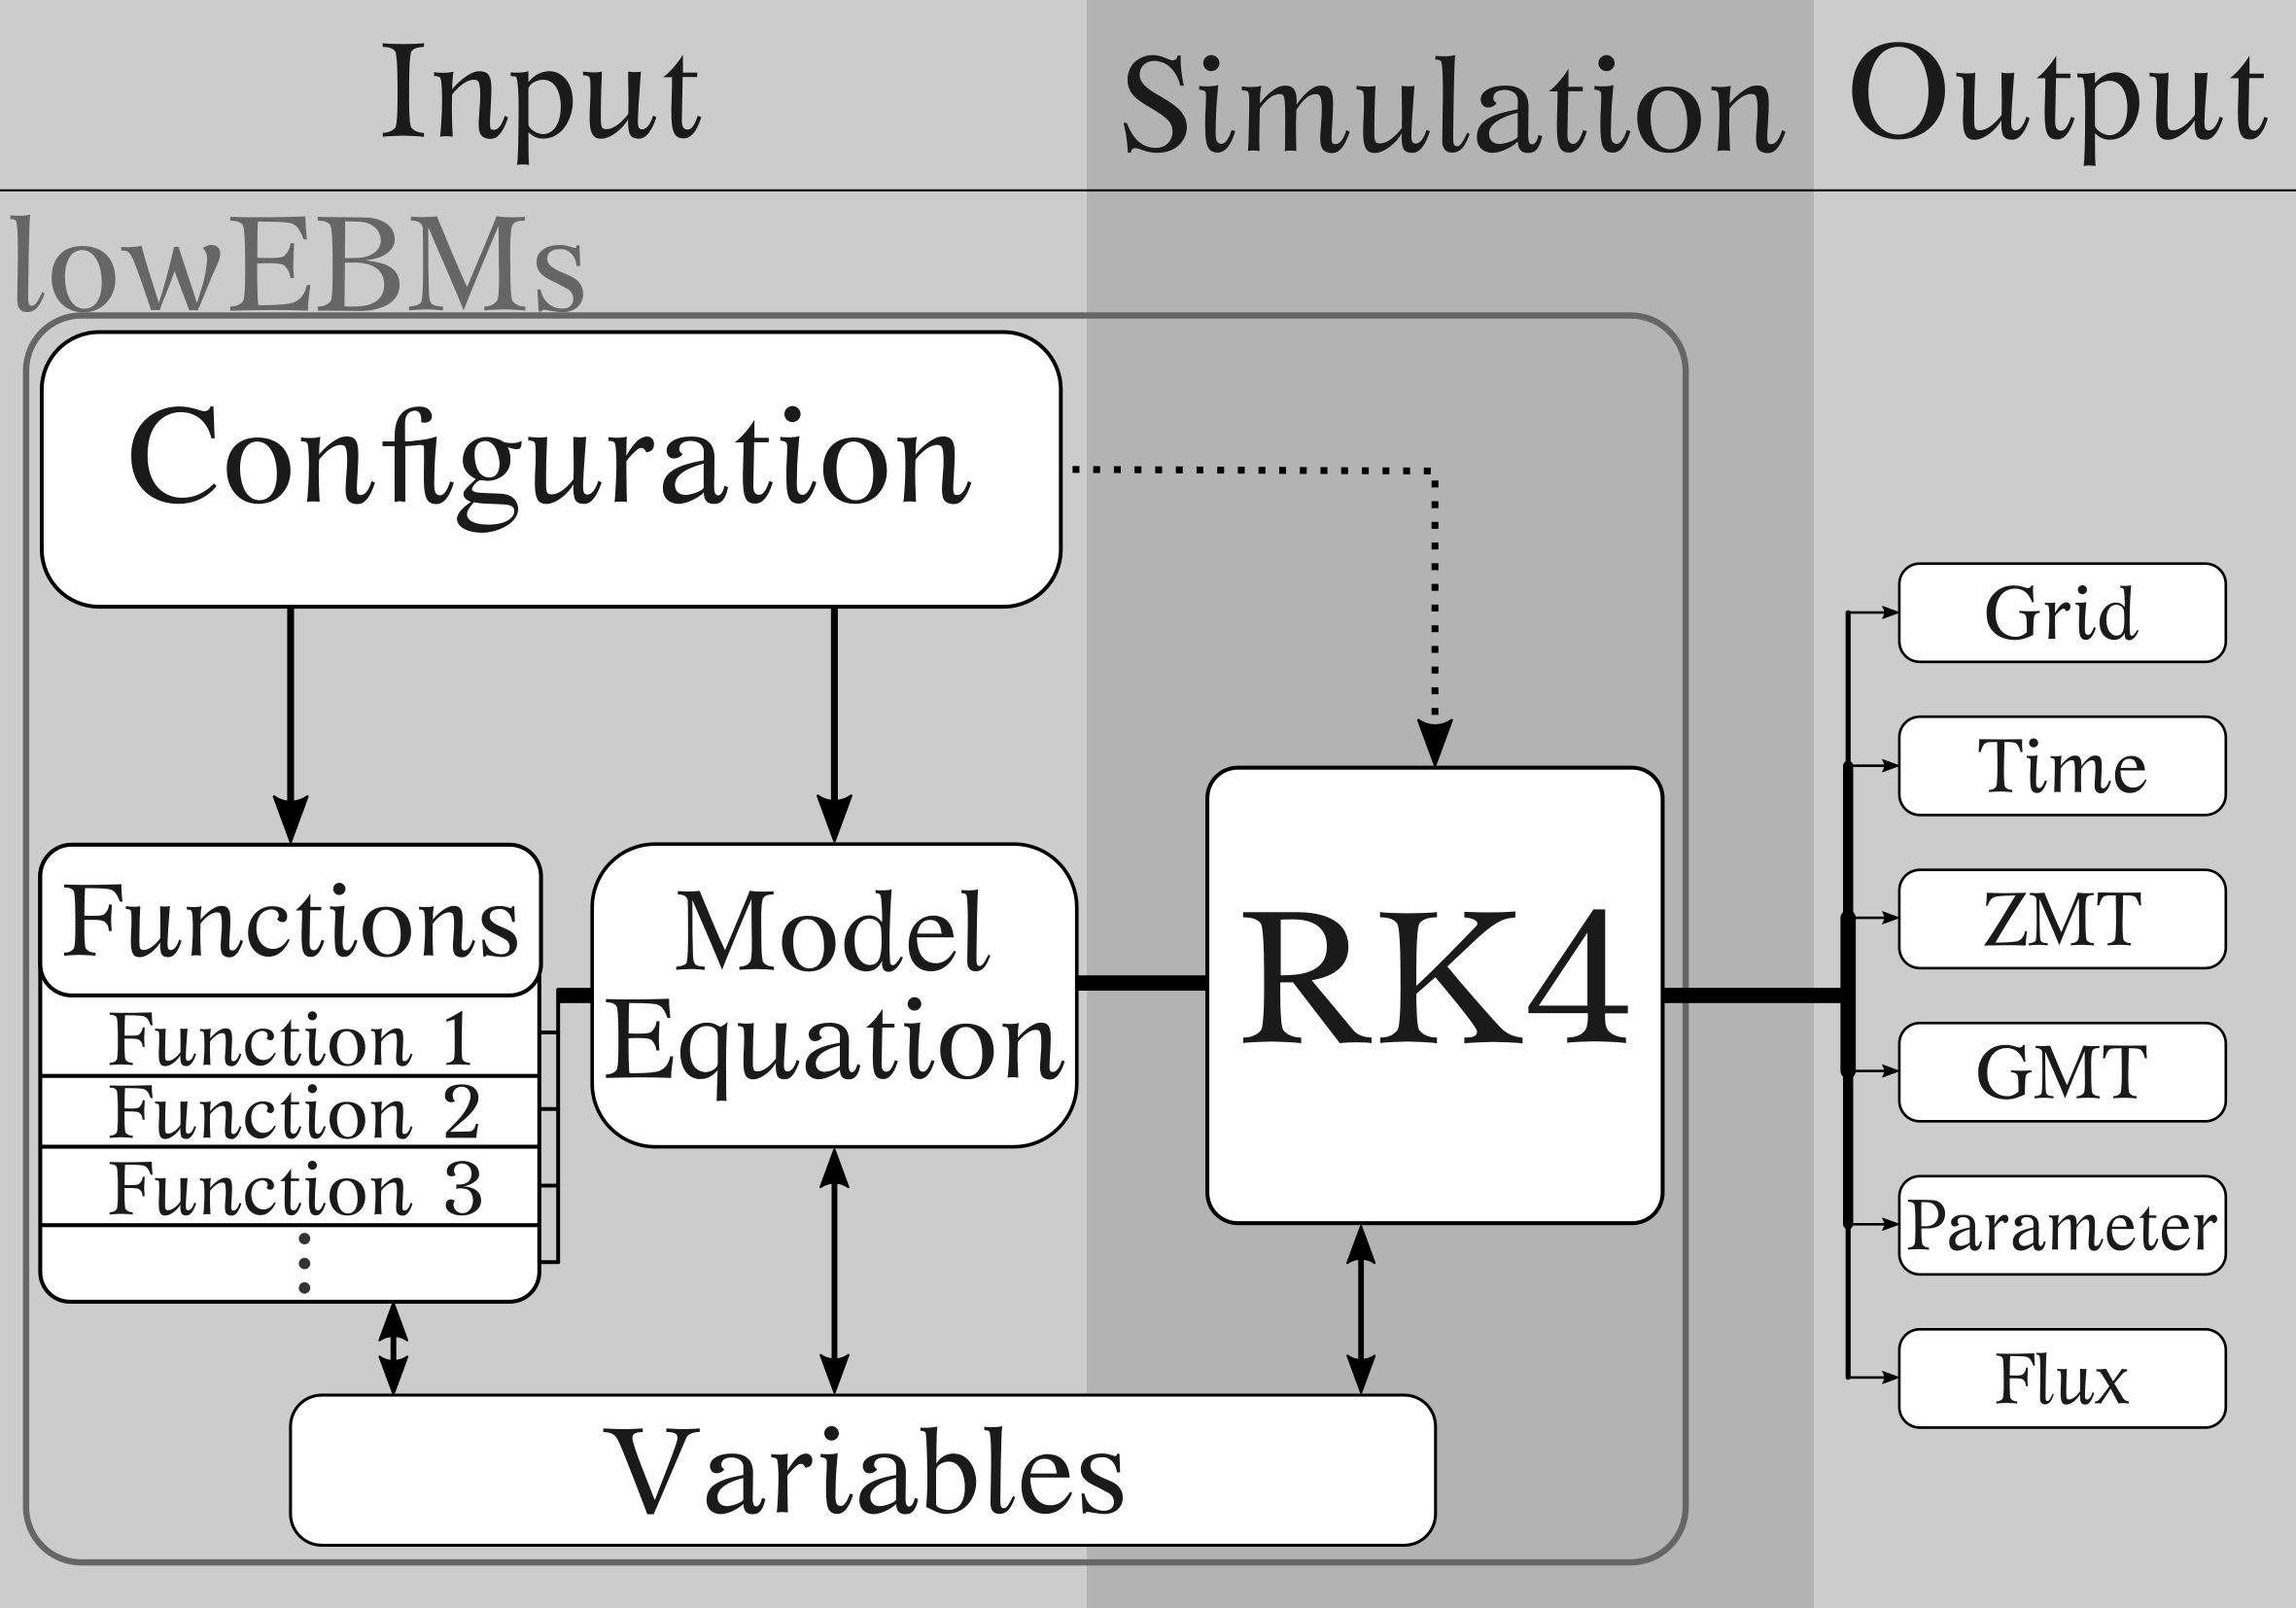
\includegraphics[width=1.1\textwidth]{Figures/Implementation/Workingmode.png}
	};
	\node[xshift=0.1cm,yshift=-0.53cm] at (current page.45) {
\includegraphics[width=0.25\textwidth]{Figures/Logos/Logo_big.png}};

    \end{tikzpicture}
\end{frame}

%\tikzstyle{nome}=[anchor=west, minimum height=\altura,minimum width=9cm,fill=yellow!30]

\begin{frame}{Implementation details - configuration}
    \begin{tikzpicture}[remember picture,overlay]
    \node[xshift=-2.9cm,yshift=-0.4cm] at (current page.center) {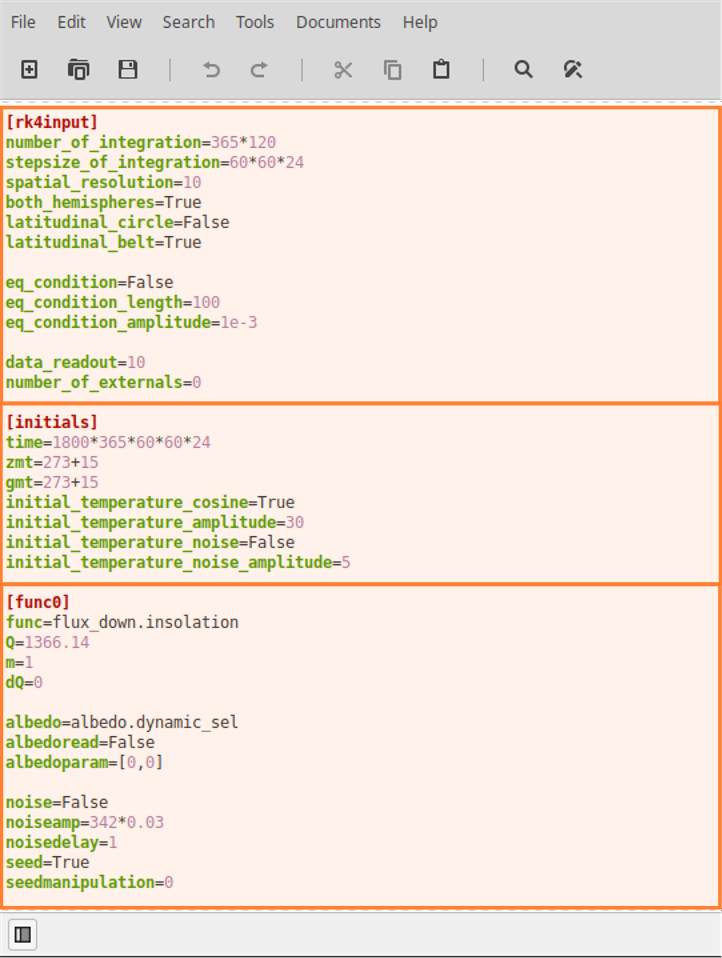
\includegraphics[width=0.55\textwidth]{Figures/Implementation/Input.png}
	};
	\node[xshift=0.1cm,yshift=-0.53cm] at (current page.45) {
\includegraphics[width=0.25\textwidth]{Figures/Logos/Logo_big.png}};
	\node[align=left,anchor=west,xshift=0.3cm,yshift=+2.5cm] at (current page.center) {$\bullet$ Input is seperated into sections};
	\node[align=left,anchor=west,xshift=0.3cm,yshift=+1.3cm] at (current page.center) {$\bullet$ Each sections variables define \\ \; the simulation};
	\node[align=left,anchor=west,xshift=0.3cm,yshift=-0.15cm] at (current page.center) {$\bullet$ [rk4input] defines the \\ numerical  integration};
	\node[align=left,anchor=west,xshift=0.3cm,yshift=-1.6cm] at (current page.center) {$\bullet$ [initial] defines the \\ initial condition};
	\node[align=left,anchor=west,xshift=0.3cm,yshift=-3.05cm] at (current page.center) {$\bullet$ [func0],..,[func4] define \\ the parameterization};
    \end{tikzpicture}
\end{frame}

\begin{frame}{Implementation details - \\ Runge-Kutta 4th order scheme}
    \begin{tikzpicture}[remember picture,overlay]
    \node[xshift=-3cm,yshift=0cm] at (current page.center) {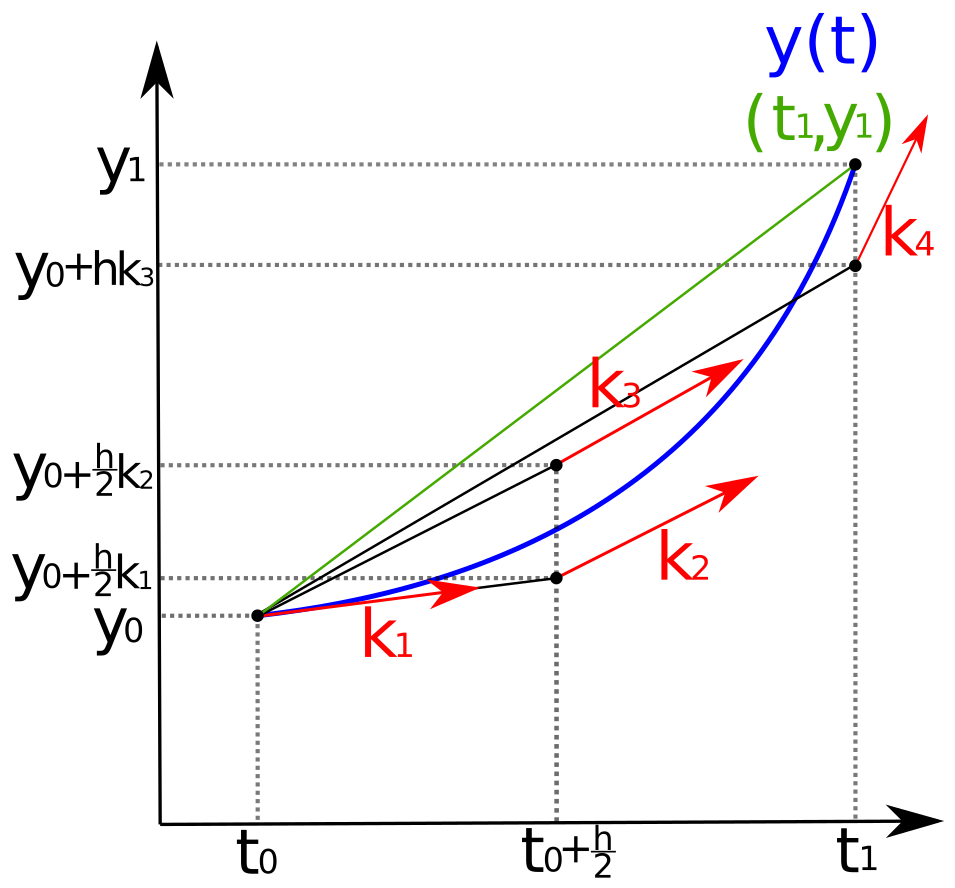
\includegraphics[width=0.5\textwidth]{Figures/Implementation/RK4.png}
	};
	\node[xshift=0.1cm,yshift=-0.53cm] at (current page.45) {
\includegraphics[width=0.25\textwidth]{Figures/Logos/Logo_big.png}};
	\node[xshift=2.8cm,yshift=+0.2cm] at (current page.center) {
            $\begin{aligned}
            k_1 &= f (t_0,y_0)\\
            k_2 &= f (t_0 + \frac{h}{2}, y_0+\frac{h}{2}\cdot k_1)\\
            k_3 &= f (t_0 + \frac{h}{2}, y_0+\frac{h}{2}\cdot k_2)\\
            k_4 &= f (t_1, y_0+h \cdot k_3)\\
            \Phi & = \frac{1}{6} k_1+\frac{1}{3} k_2+\frac{1}{3} k_3+\frac{1}{6} k_4\\
            \\
            y_1 &=y_0 + \Phi (f,t_0,y_0,h) \cdot h 
            \end{aligned}$
	};
	\node[xshift=0cm,yshift=-3.6cm] at (current page.center) {$\bullet$ iteratively solve the model equation (with $f(t,y)\hat{=}\frac{dT}{dt}$)};
    \end{tikzpicture}
\end{frame}

\begin{frame}{Implementation details - documentation}
    \begin{tikzpicture}[remember picture,overlay]
    \node[xshift=0cm,yshift=0cm] at (current page.center) {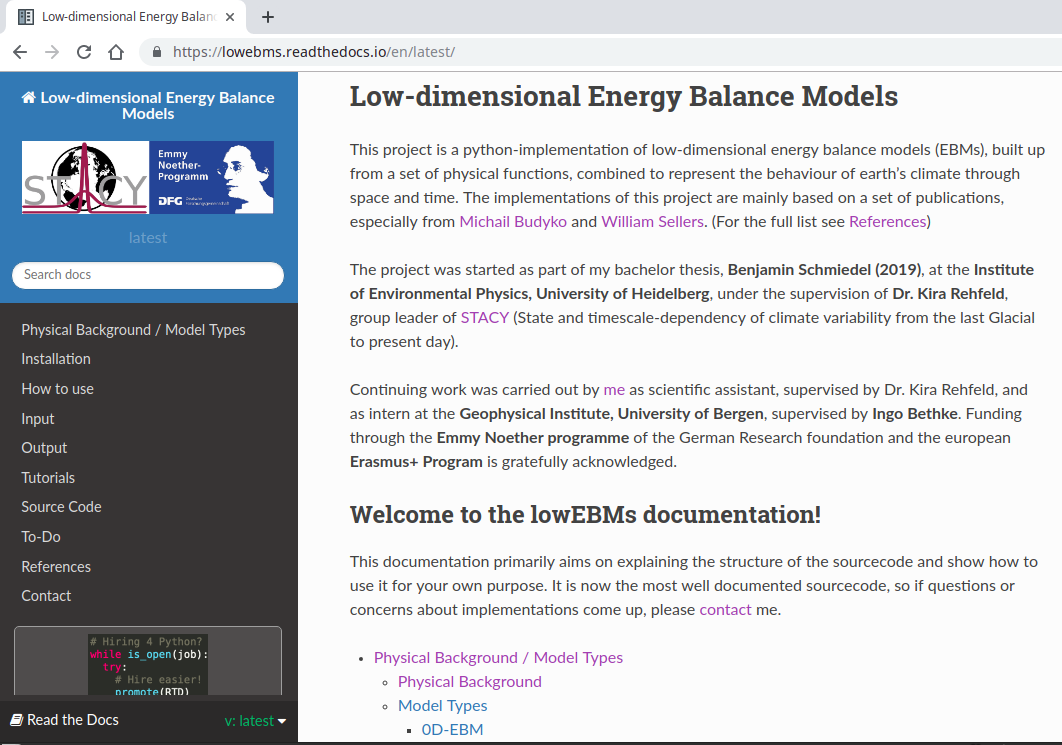
\includegraphics[width=0.85\textwidth]{Figures/Implementation/Docu.png}
	};
	\node[draw,xshift=0,yshift=-4cm] at (current page.center) {\url{https://lowebms.readthedocs.io/en/latest/}};
	\node[xshift=0.1cm,yshift=-0.53cm] at (current page.45) {
\includegraphics[width=0.25\textwidth]{Figures/Logos/Logo_big.png}};

    \end{tikzpicture}
\end{frame}

\begin{comment}
\begin{frame}{Application period}
    \begin{itemize}
        \item Timeframe
        \item Record of volcanic eruptions
        \item Variation in the TSI
        \item Importance of orbital parameters?
        \item CO2,...?
    \end{itemize}
\end{frame}
\end{comment}

\section{Application period}

\begin{frame}{Application period - Late Holocene}
	\begin{tikzpicture}[remember picture,overlay]
    \onslide<1>{\node[xshift=0cm,yshift=-0.5cm] at (current page.center) {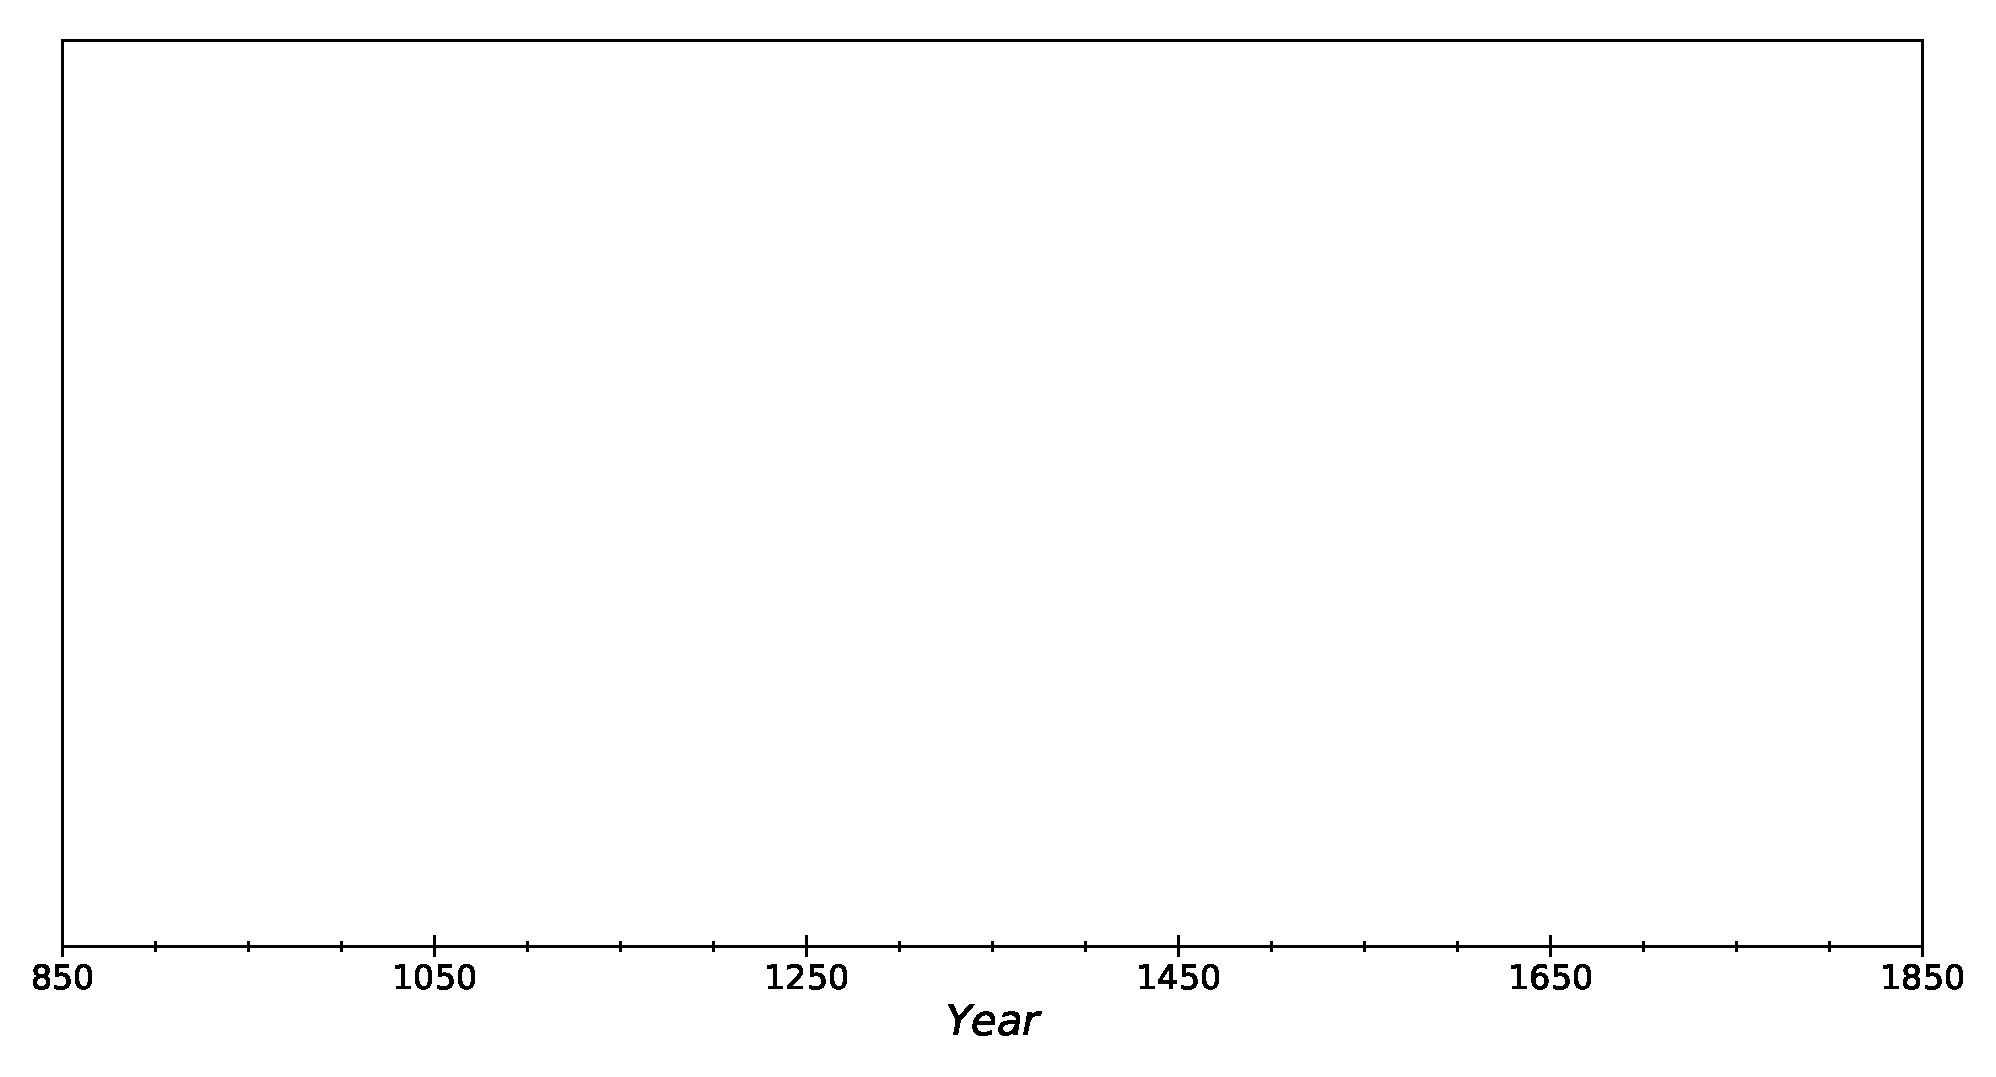
\includegraphics[width=1\textwidth]{Figures/ApplicationPeriod/Period_empty.eps}
	};}
	\onslide<2>{\node[xshift=0.25cm,yshift=-0.5cm] at (current page.center) {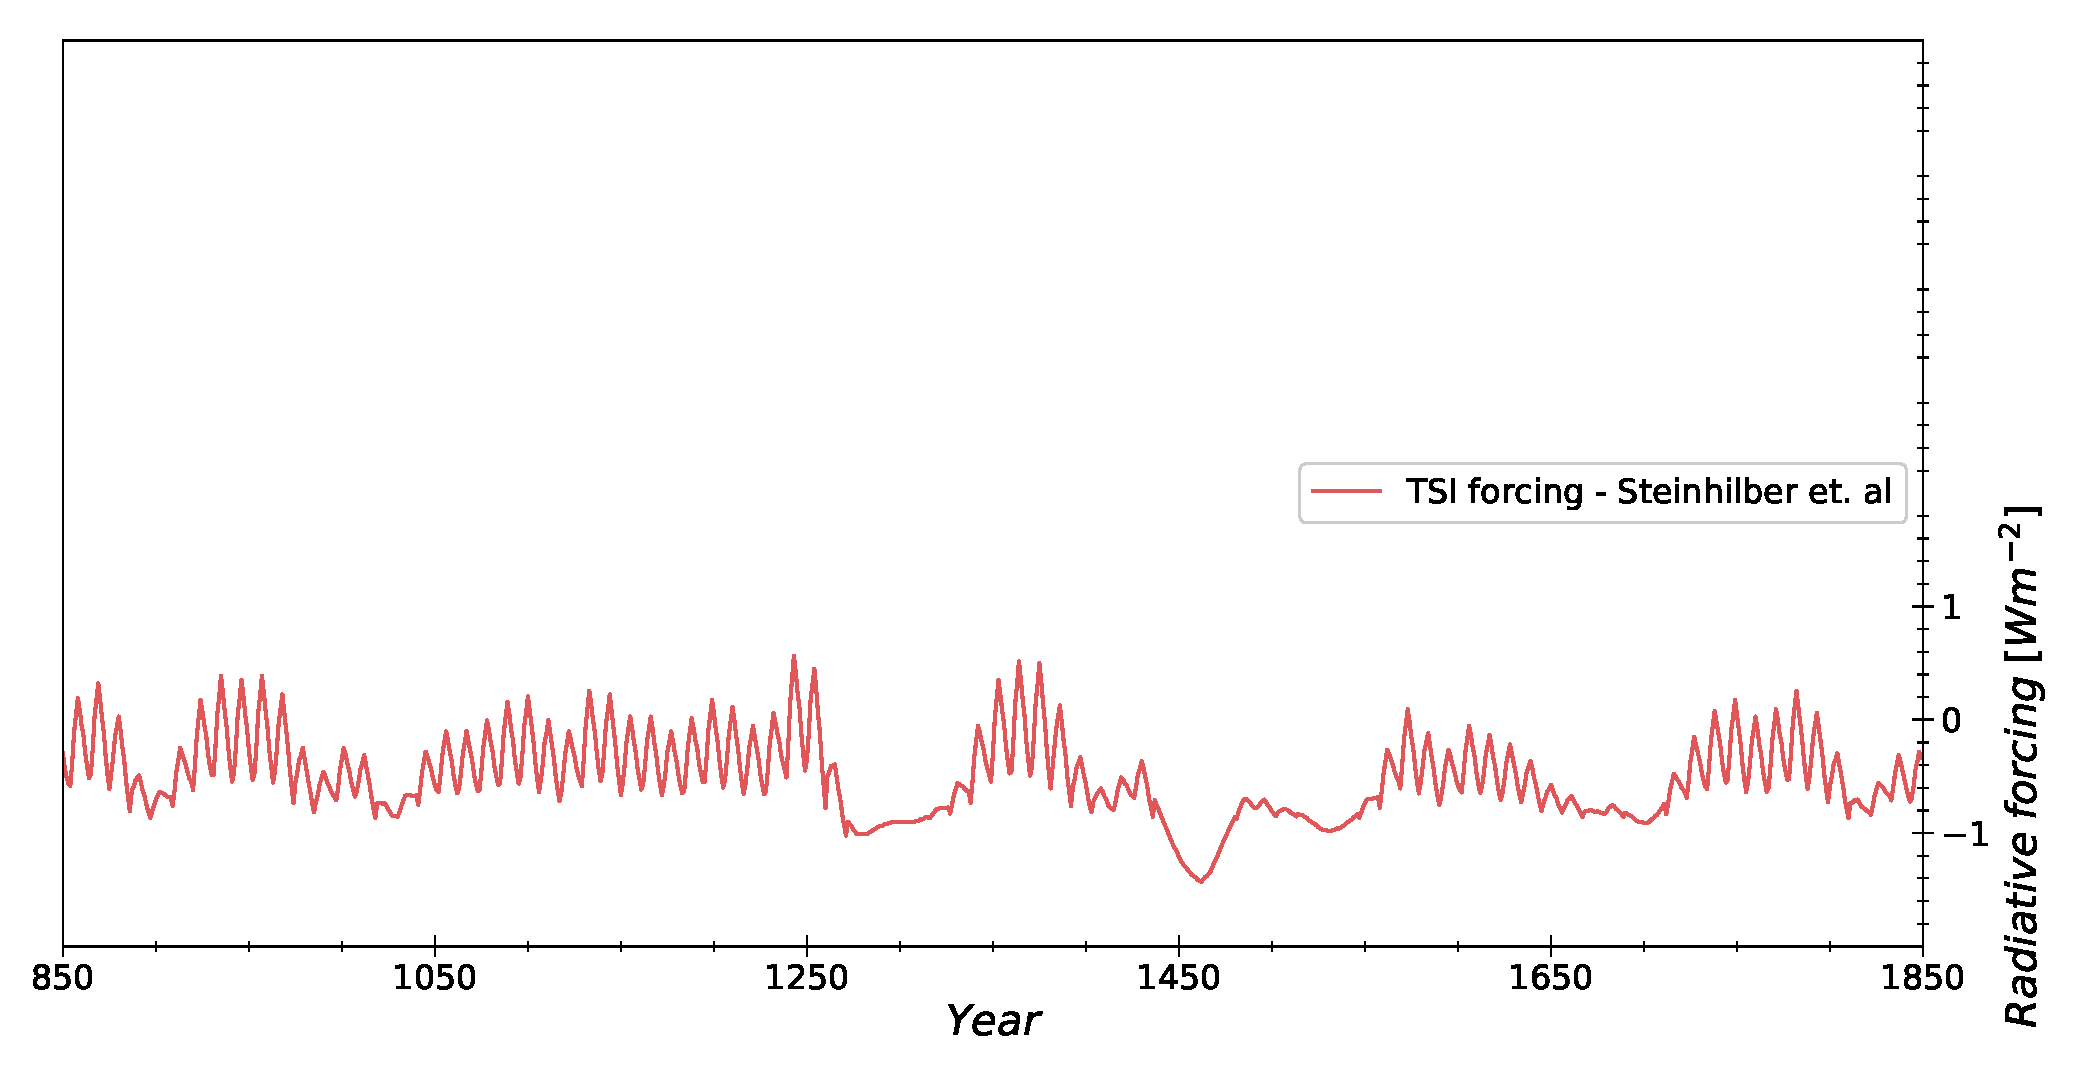
\includegraphics[width=1.05\textwidth]{Figures/ApplicationPeriod/Period_TSI.eps}
	};}
	\onslide<3->{\node[xshift=0cm,yshift=-0.5cm] at (current page.center) {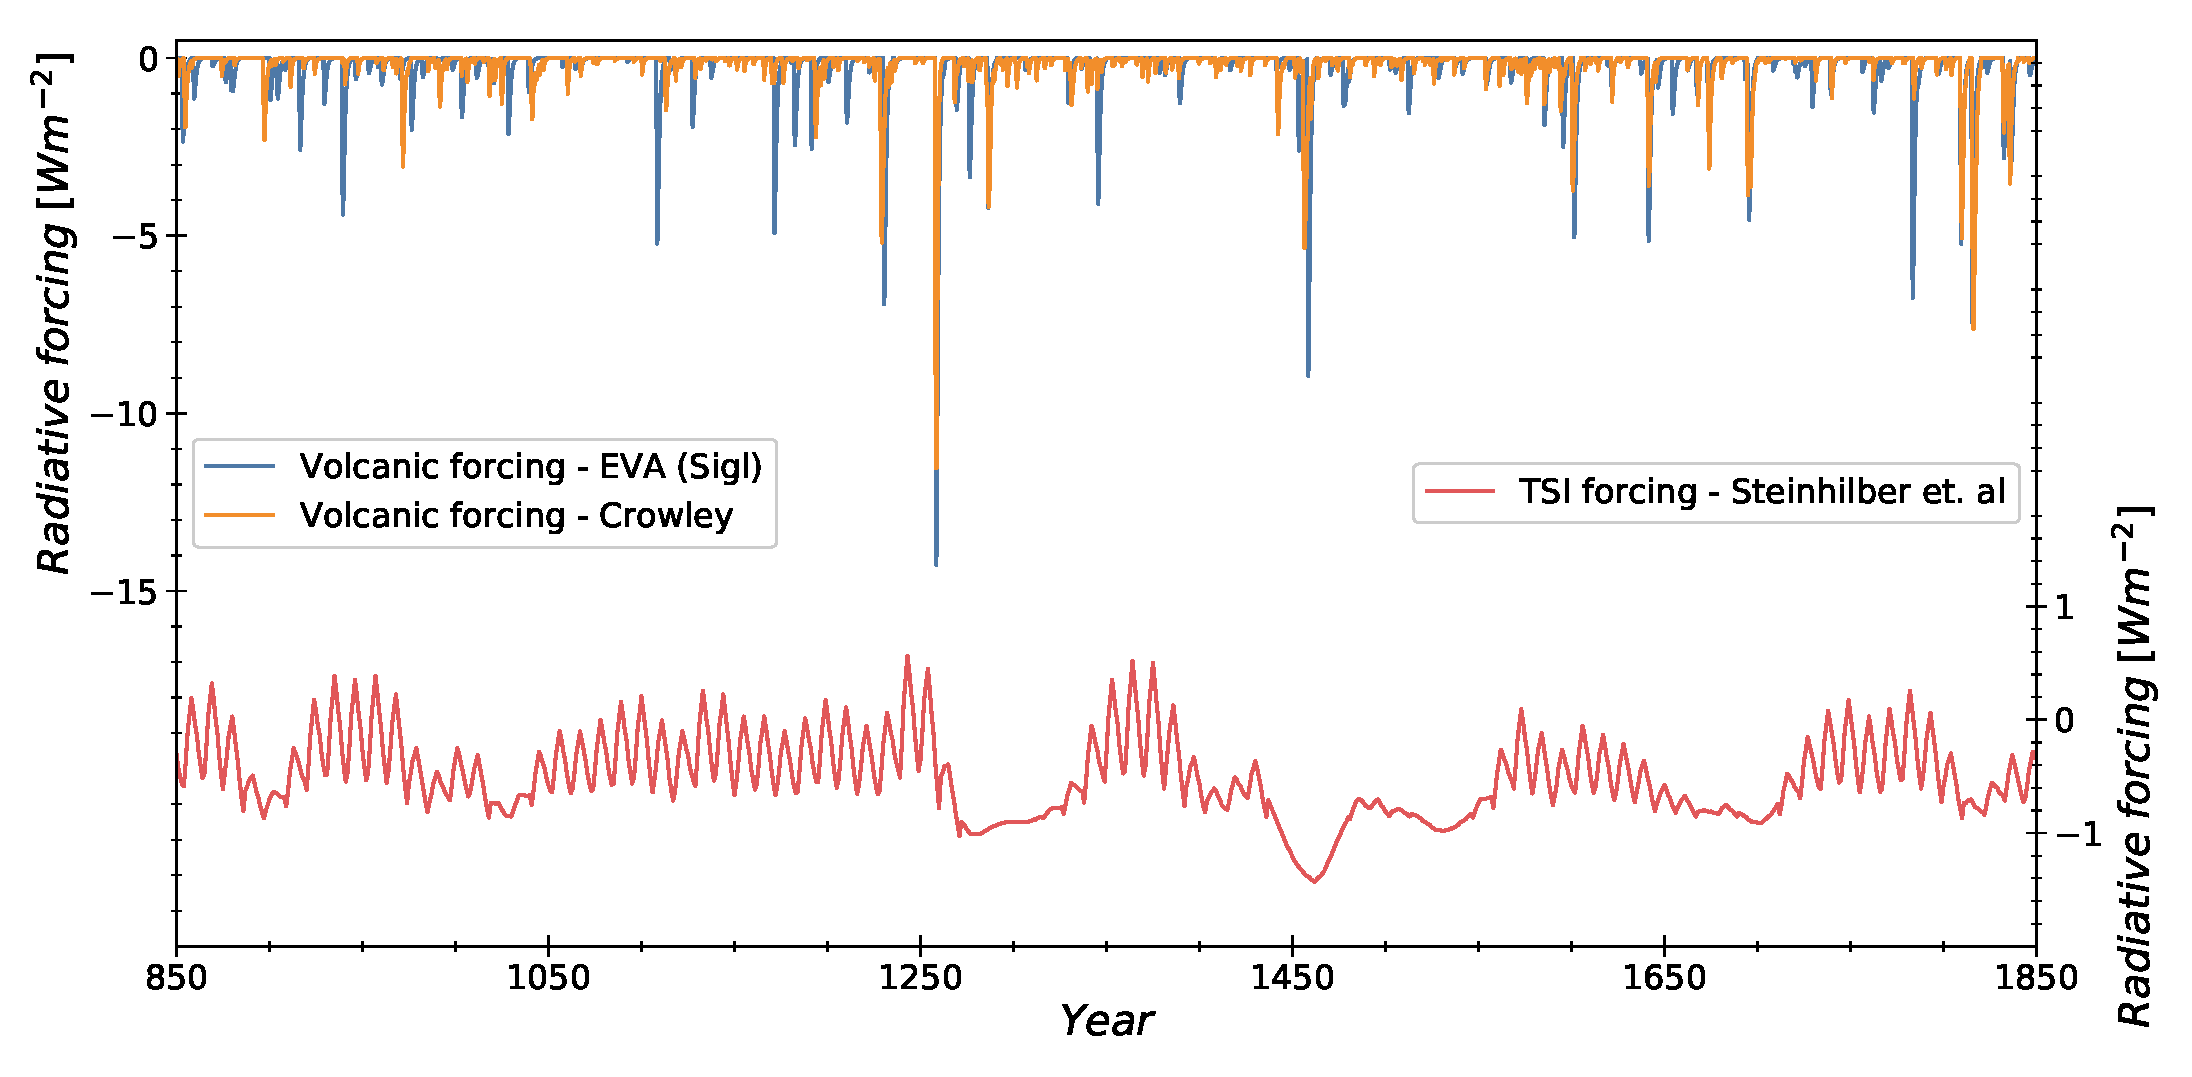
\includegraphics[width=1.1\textwidth]{Figures/ApplicationPeriod/Period_Volc_TSI.eps}
	};}
	\onslide<4>{\node[xshift=-0cm, yshift=0cm] at (current page.center){
	\mybox{
	\begin{align*}
	C \frac{dT}{dt} = R_{\downarrow}  - R_{\uparrow} + F_{transfer} + F_{forcing}\\
	\end{align*}}};}
    \end{tikzpicture}
    \onslide<3>{\blfootnote{[Steinhilber 2009, Sigl 2015, Toohey 2016, Crowley 2008]}}
\end{frame}

\section{Practical demonstration [Jupyter Notebook]}

\begin{frame}{Jupyter notebook demonstration}
    Screen Change
\end{frame}

\section{Additional features}

\begin{comment}
\begin{frame}{Additional features}
    \begin{itemize}
        \item ForcingGenerator (0D, 1D, resample)
        \item Ensemble Runs (Example with different mixedlayer depths?)
        \item Optimization alogrithm for parameter optimization (Gradient descent)
        \item 
    \end{itemize}
\end{frame}
\end{comment}

\begin{frame}{Additional features - Overview}
    \begin{tikzpicture}[remember picture,overlay]
    \node[xshift=-0cm, yshift=0cm] at (current page.center) {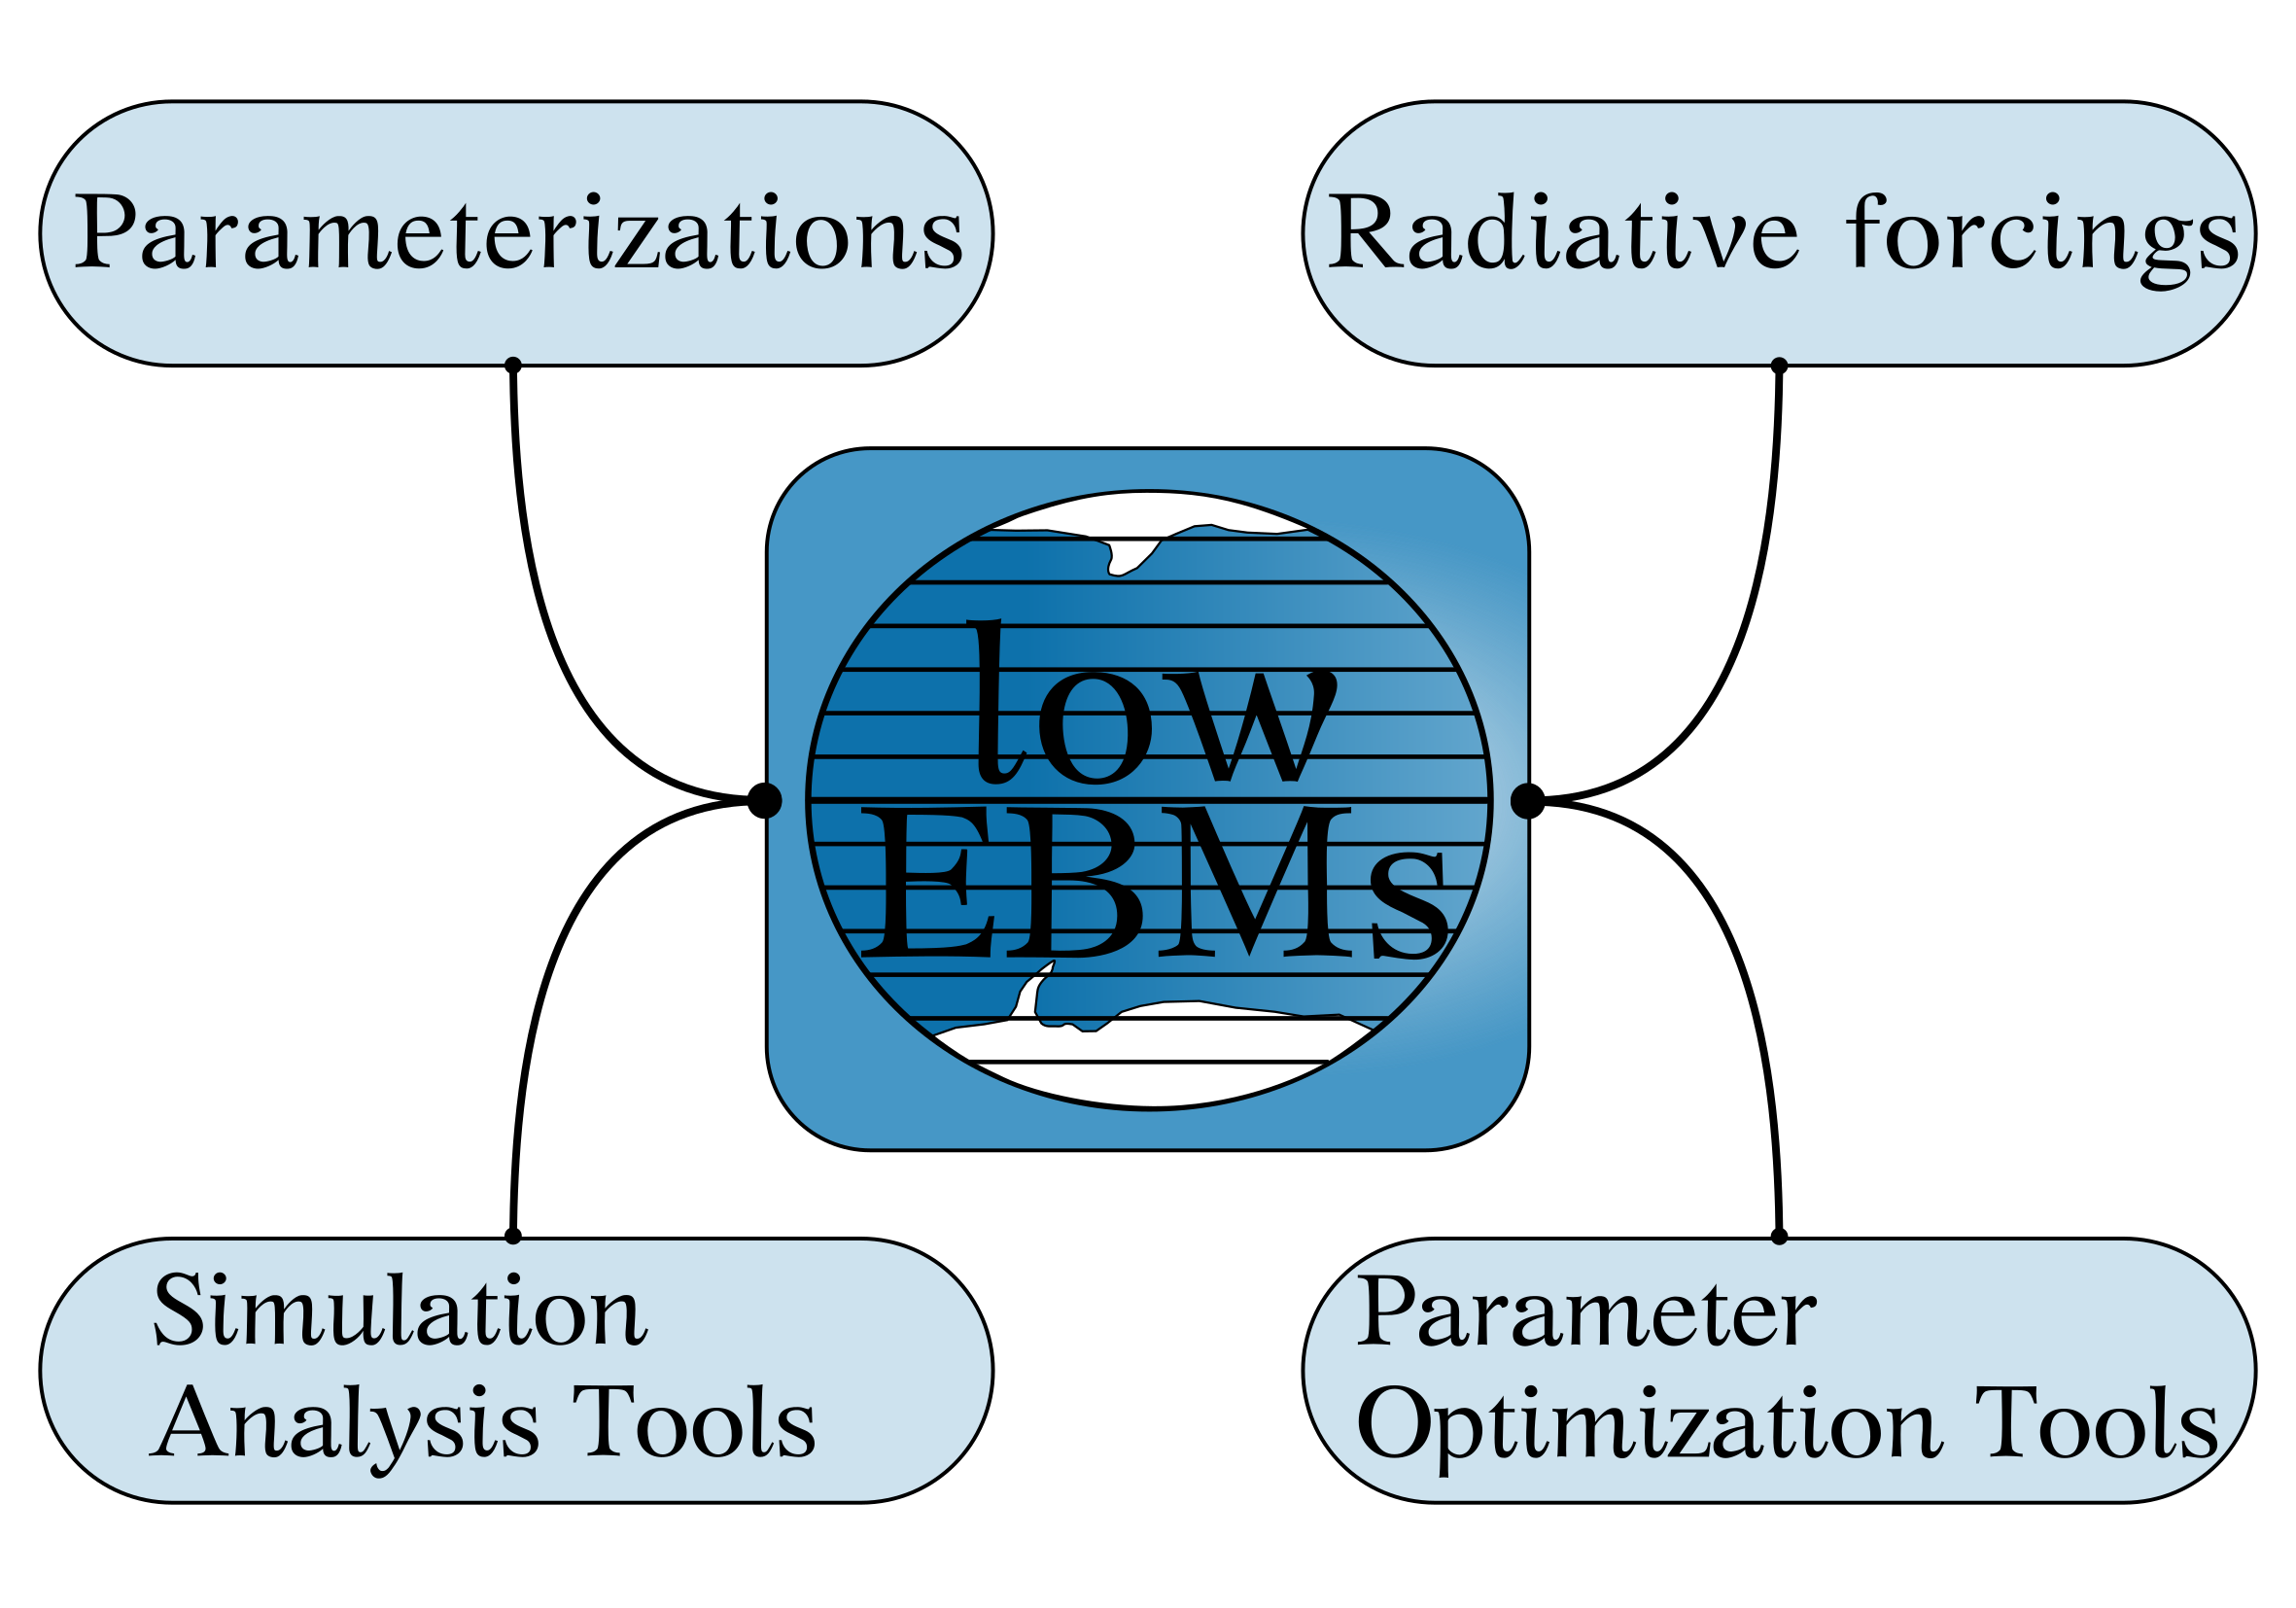
\includegraphics[width=\textwidth]{Figures/Motivation/Content_Map.png}};
    \end{tikzpicture}
\end{frame}

\begin{frame}{Additional features - VolcanicForcingGenerator}
    \begin{tikzpicture}[remember picture,overlay]
	\node[xshift=2.45cm,yshift=-2.2cm] at (current page.center) {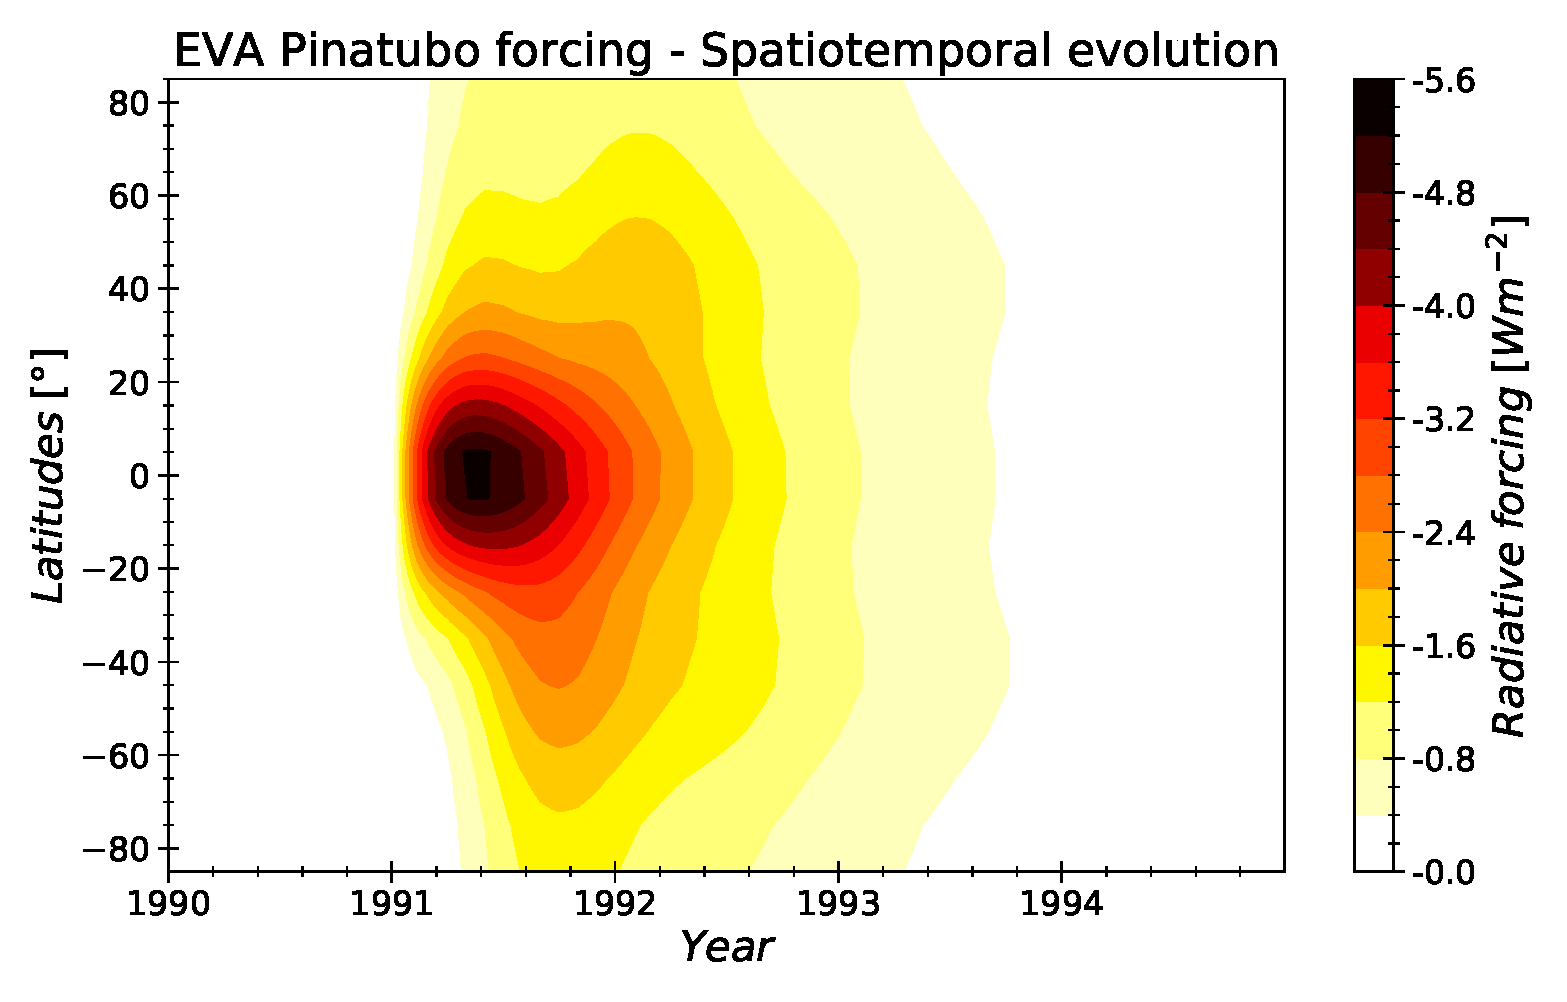
\includegraphics[width=0.63\textwidth]{Figures/Applications/Spatiotemporal_evolution_EVA.eps}
	};
	\node[xshift=-2.9cm,yshift=1.0cm] at (current page.center) {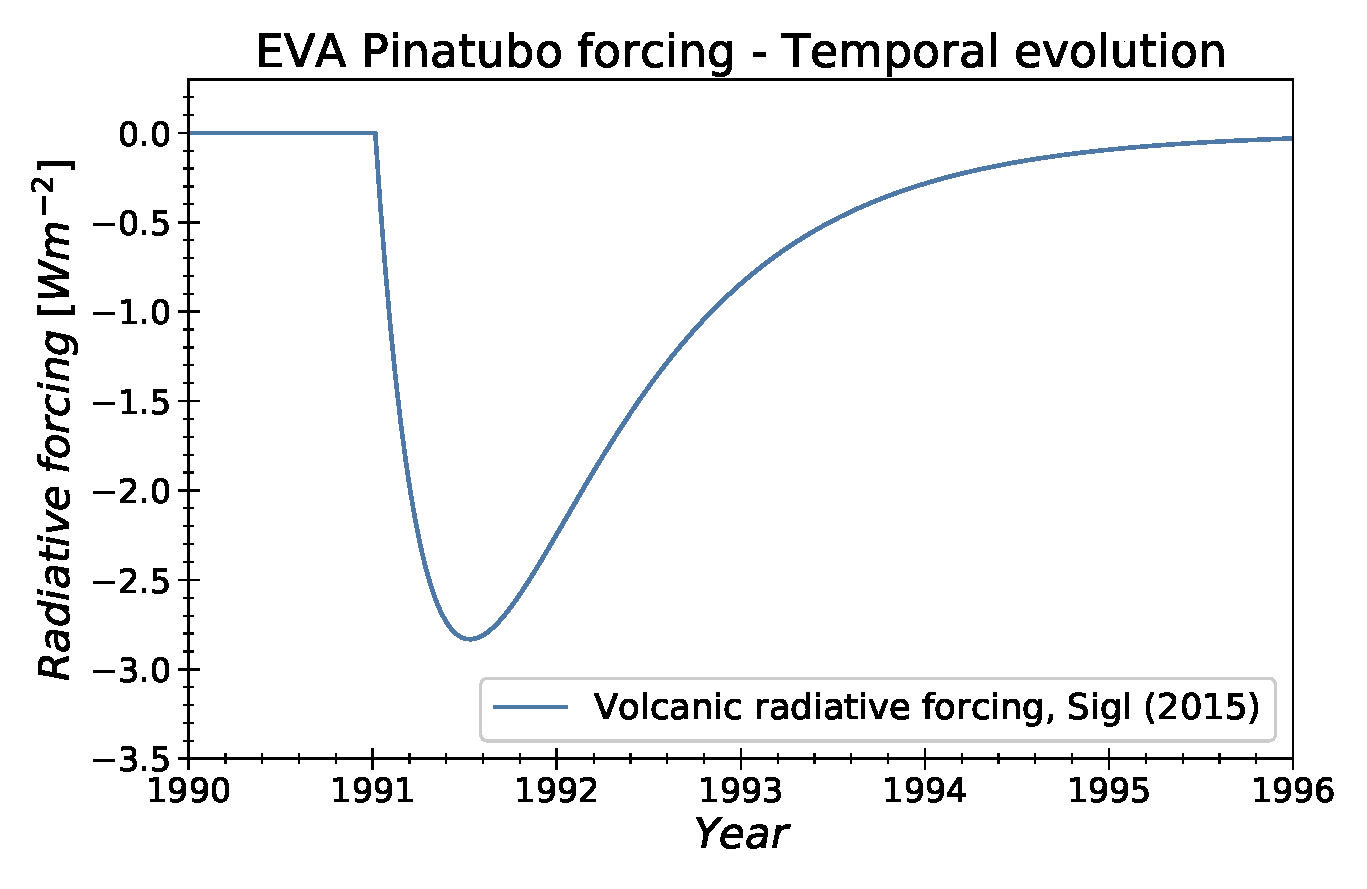
\includegraphics[width=0.56\textwidth]{Figures/Applications/Temporal_evolution_EVA.eps}
	};	
    %\node[anchor=west,align=left,xshift=1cm,yshift=2cm] at (current page.center) {\footnotesize{$\bullet$}\normalsize\; Estimates the spatiotemporal\\ \;\;
    %evolution of sulfur\\  converts it to radiative  \\ 
    %\;\; to AOD / radiative forcing
    %};
    %\node[anchor=west,align=left,xshift=-6cm,yshift=-2.6cm] at (current page.center) {\footnotesize{$\bullet$}\normalsize };
    \end{tikzpicture}
\end{frame}

\begin{frame}{Additional features - VolcanicForcingGenerator}
    \begin{tikzpicture}[remember picture,overlay]
	\node[xshift=0cm,yshift=-0.3cm] at (current page.center) {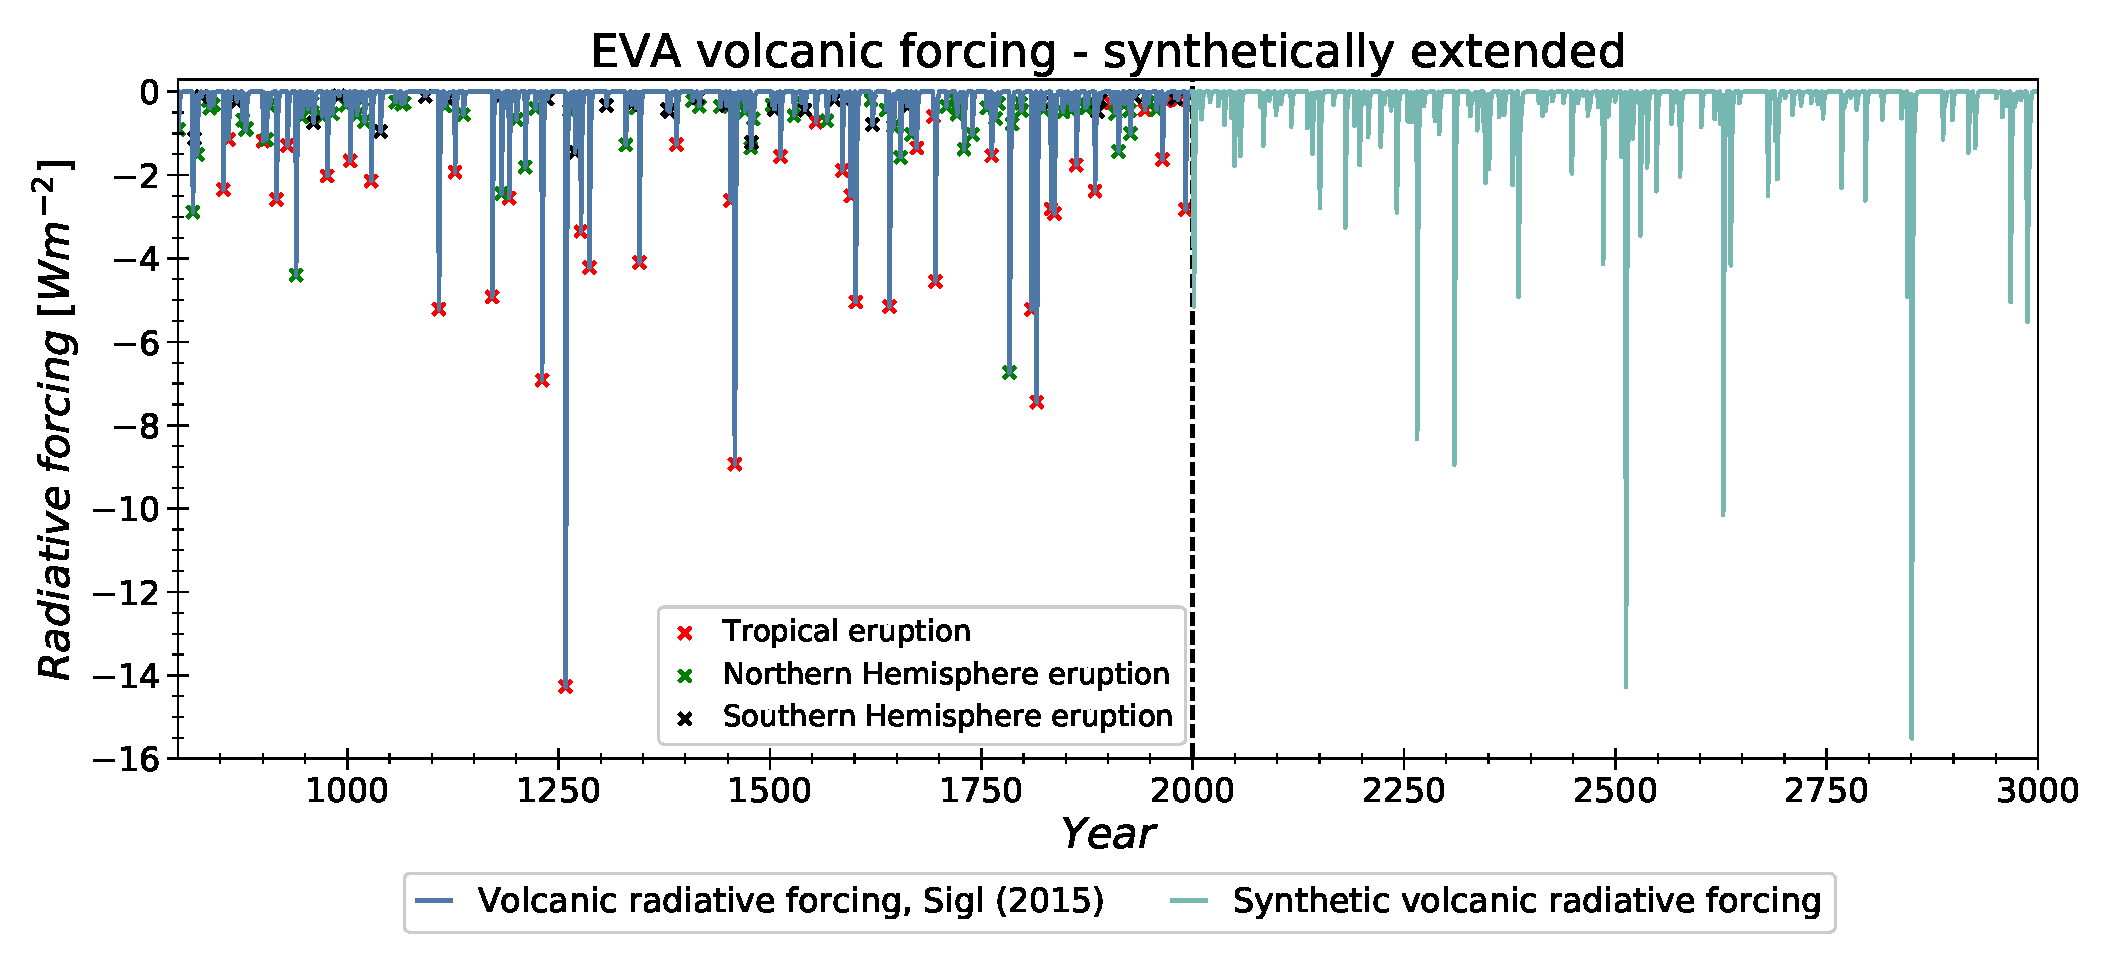
\includegraphics[width=1.1\textwidth]{Figures/Applications/EVA_extended.eps}
	};
    \end{tikzpicture}
\end{frame}

\begin{frame}{Additional features - Simulation analysis tools: Ensemble}
    \begin{tikzpicture}[remember picture,overlay]
    \node[xshift=-2.7cm,yshift=1.5cm] at (current page.center) {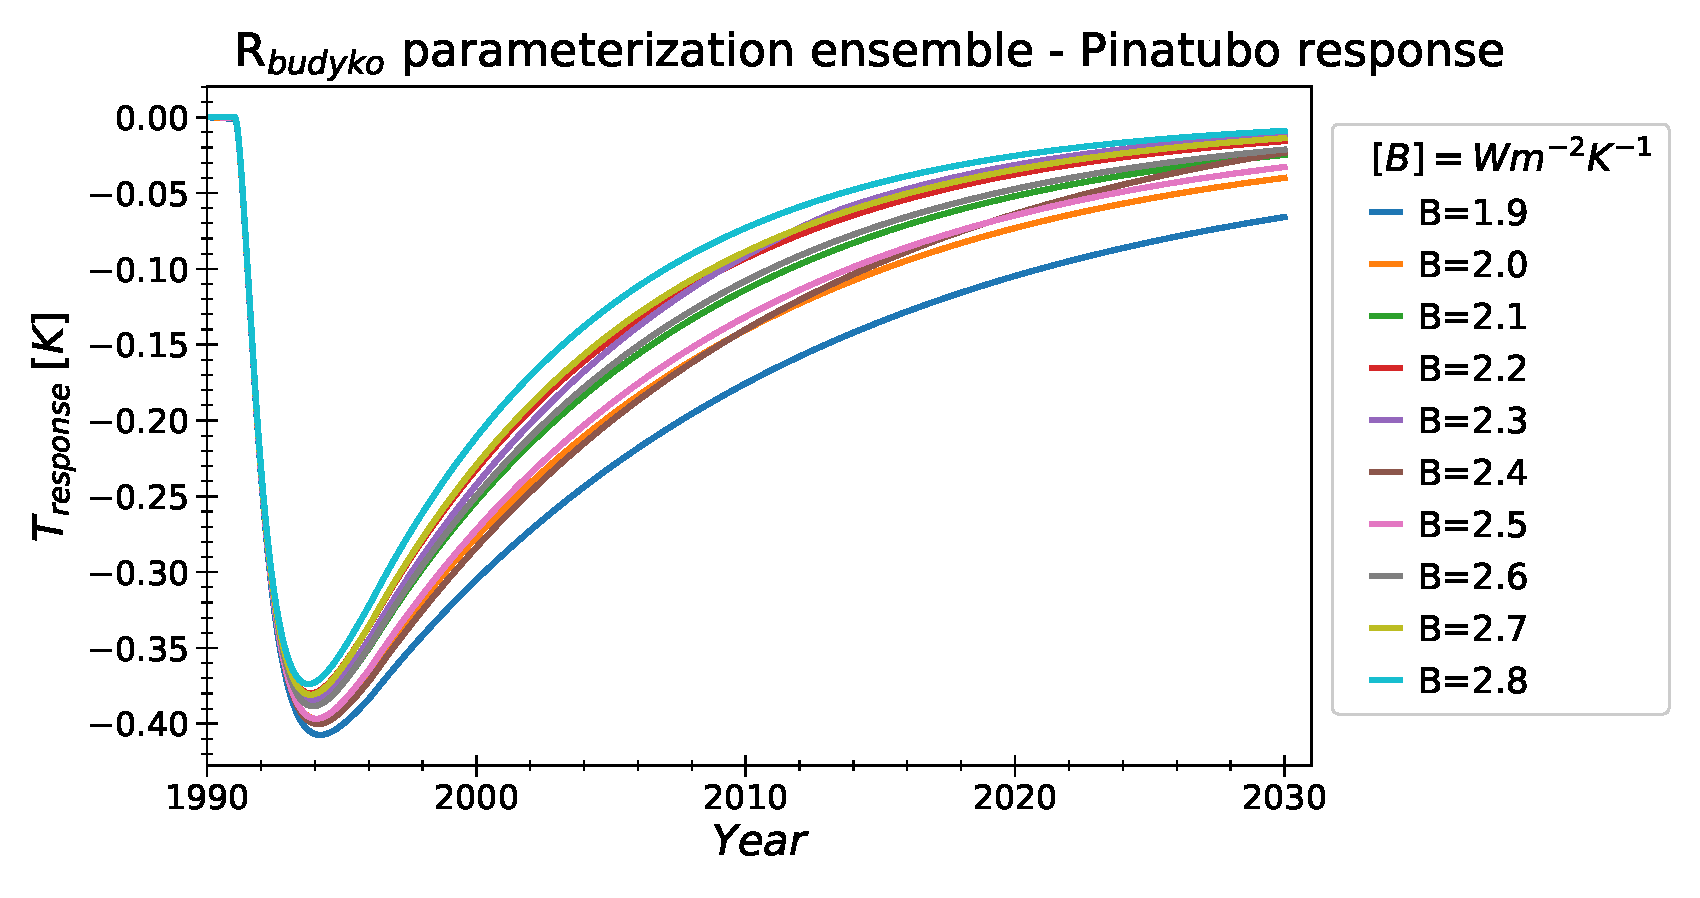
\includegraphics[width=0.65\textwidth]{Figures/Applications/EnsembleParameters_Response.eps}
	};
	\node[xshift=2.6cm,yshift=-2.2cm] at (current page.center) {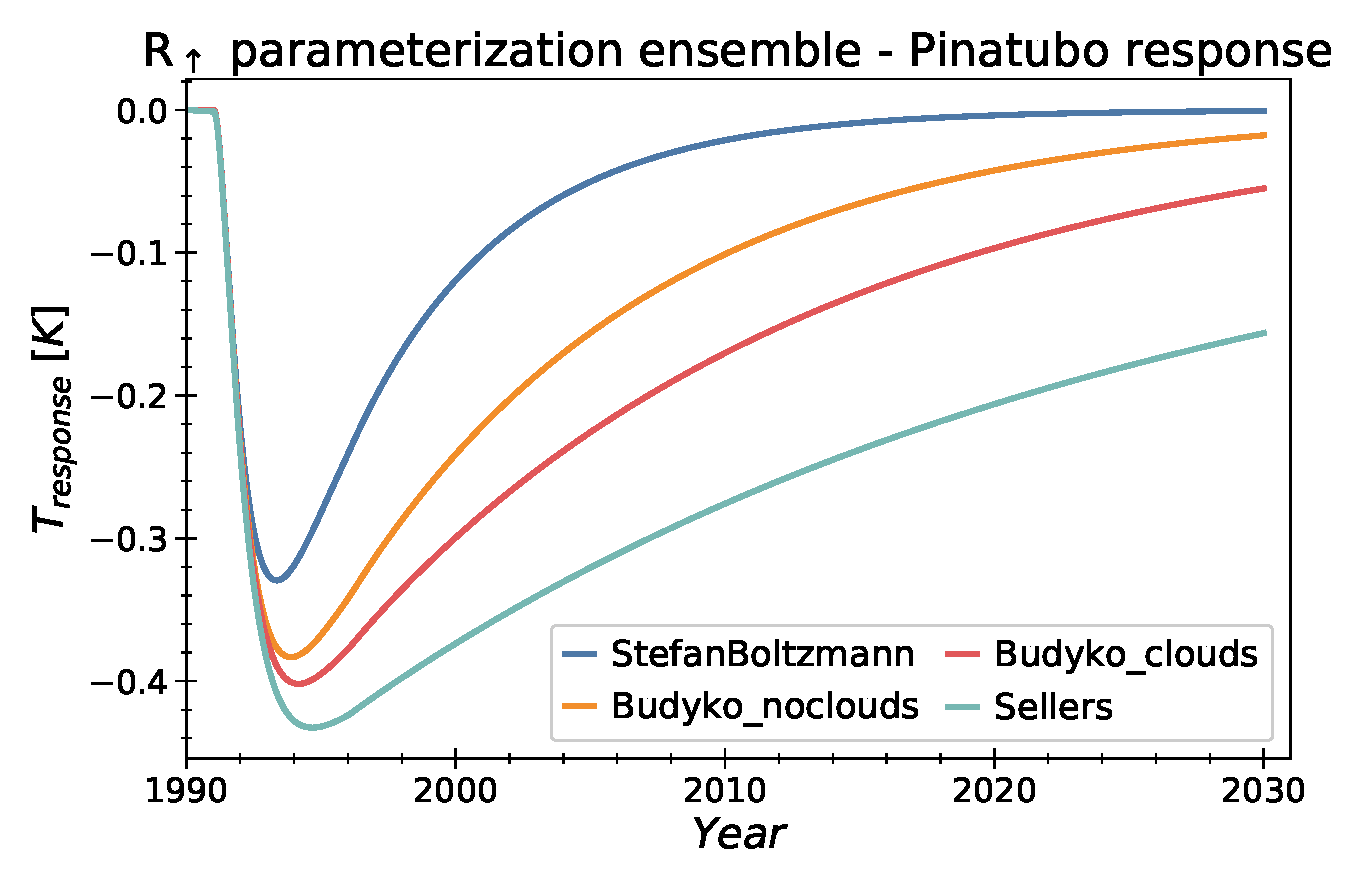
\includegraphics[width=0.6\textwidth]{Figures/Applications/Ensemble_Response.eps}
	};
    \end{tikzpicture}
\end{frame}

\begin{frame}{Additional features - Parameter optimization tools}
    \begin{tikzpicture}[remember picture,overlay]
    \node[anchor=west,xshift=-6cm,yshift=2.6cm] at (current page.center) {\footnotesize{$\bullet$}\normalsize\; Optimization Method:\; Gradient descent};
    \node[anchor=west,xshift=-6cm,yshift=1.6cm] at (current page.center) {\footnotesize{$\bullet$}\normalsize\; Cost function:\; Least squares};
    \node[xshift=-2.5cm,yshift=-1.8cm] at (current page.center) {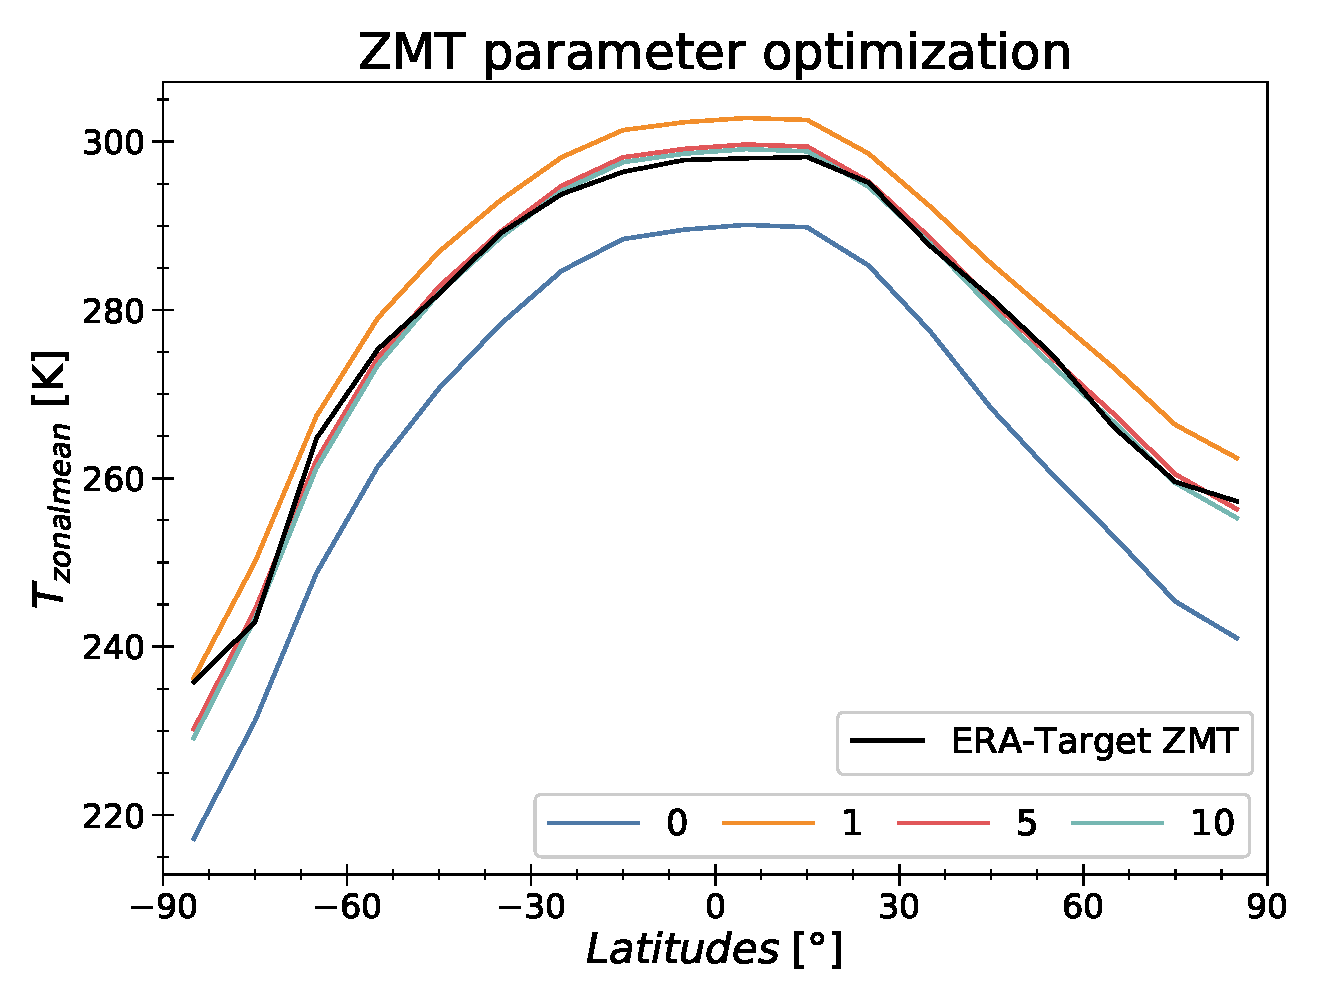
\includegraphics[width=0.63\textwidth]{Figures/Applications/ZMT_Optimization_Sellers.eps}
	};
	\node[xshift=3.7cm,yshift=1.2cm] at (current page.center) {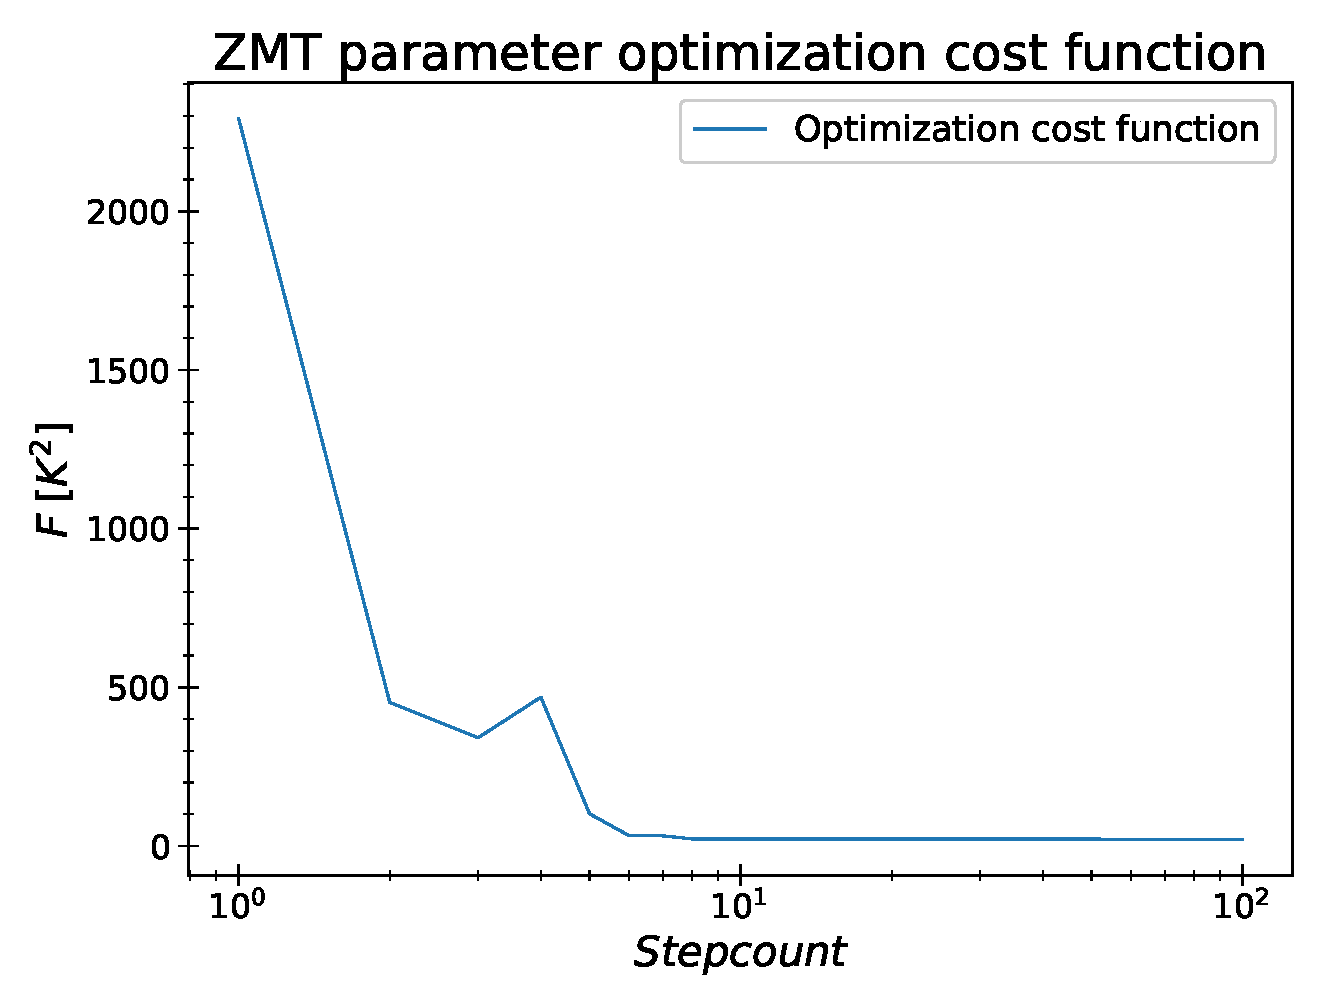
\includegraphics[width=0.38\textwidth]{Figures/Applications/ZMT_Optimization_F.eps}
	};
	\node[xshift=3.8cm,yshift=-2.1cm] at (current page.center) {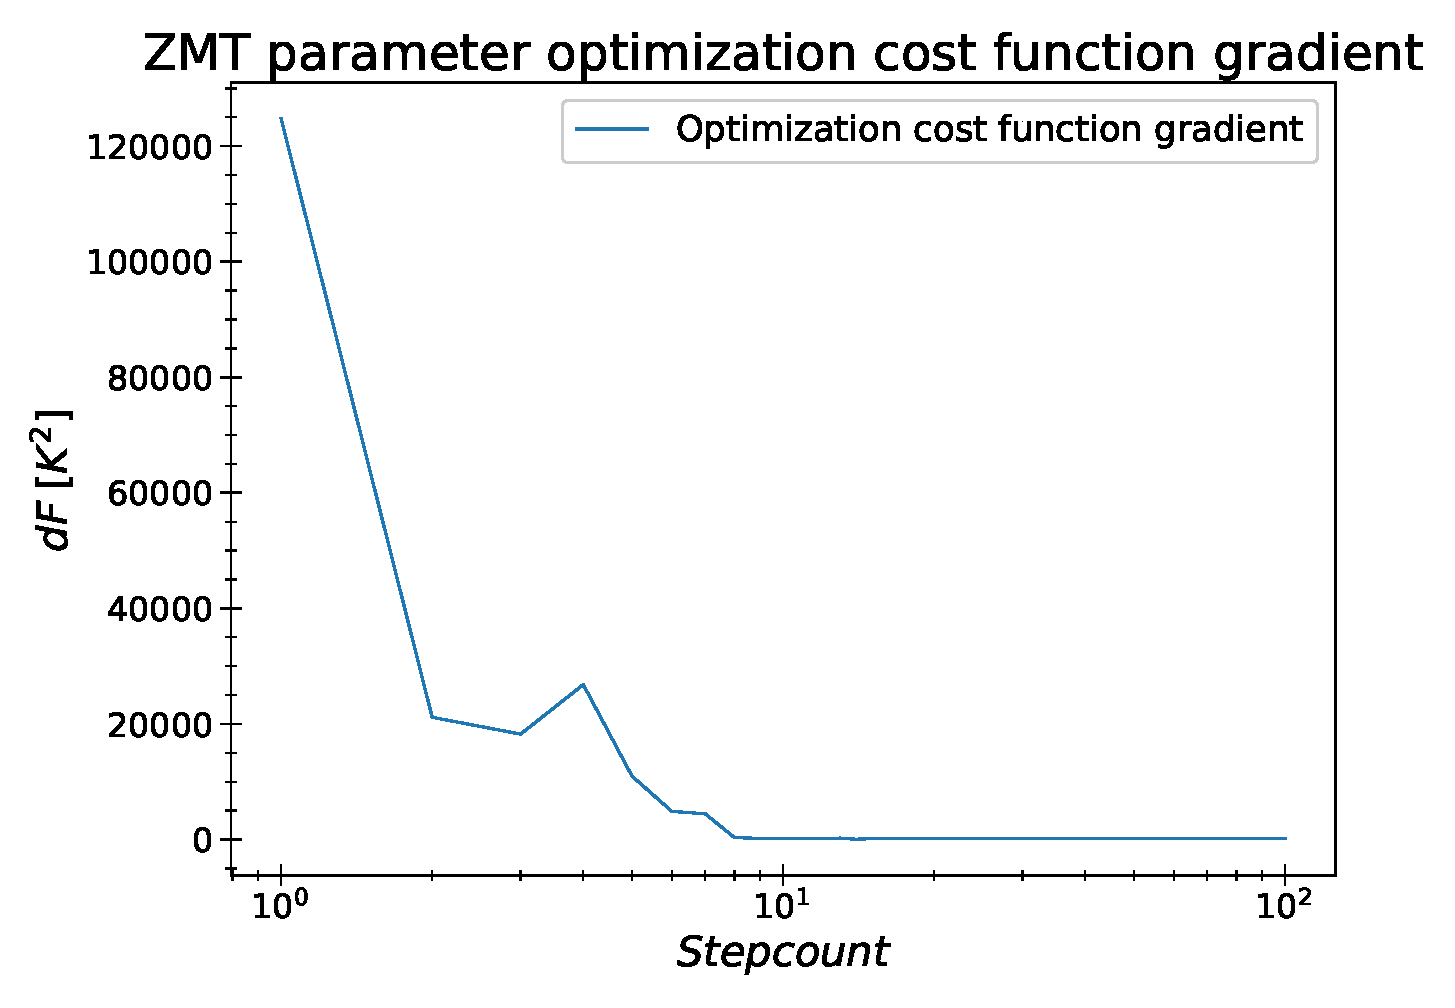
\includegraphics[width=0.42\textwidth]{Figures/Applications/ZMT_Optimization_dF.eps}
	};
    \end{tikzpicture}
\end{frame}

\section{Outlook}

\begin{frame}{Outlook}
	\begin{tikzpicture}[remember picture,overlay]
	\node[align=left,anchor=west,xshift=-5.6cm,yshift=+2.7cm] at (current page.center) {
	$\bullet$ Tune parameterization to adapt to GCM/observation data};
	\node[align=left,anchor=west,xshift=-5.6cm,yshift=+1.7cm] at (current page.center) {
	$\bullet$ Perform simulations over long timescales (LGP, LGM, Pliocene)};
	\node[align=left,anchor=west,xshift=-5.6cm,yshift=0.7cm] at (current page.center) {
	$\bullet$ Test various parameterizations and their climatic behaviour};
	
	\node[xshift=3cm,yshift=-2cm] at (current page.center) {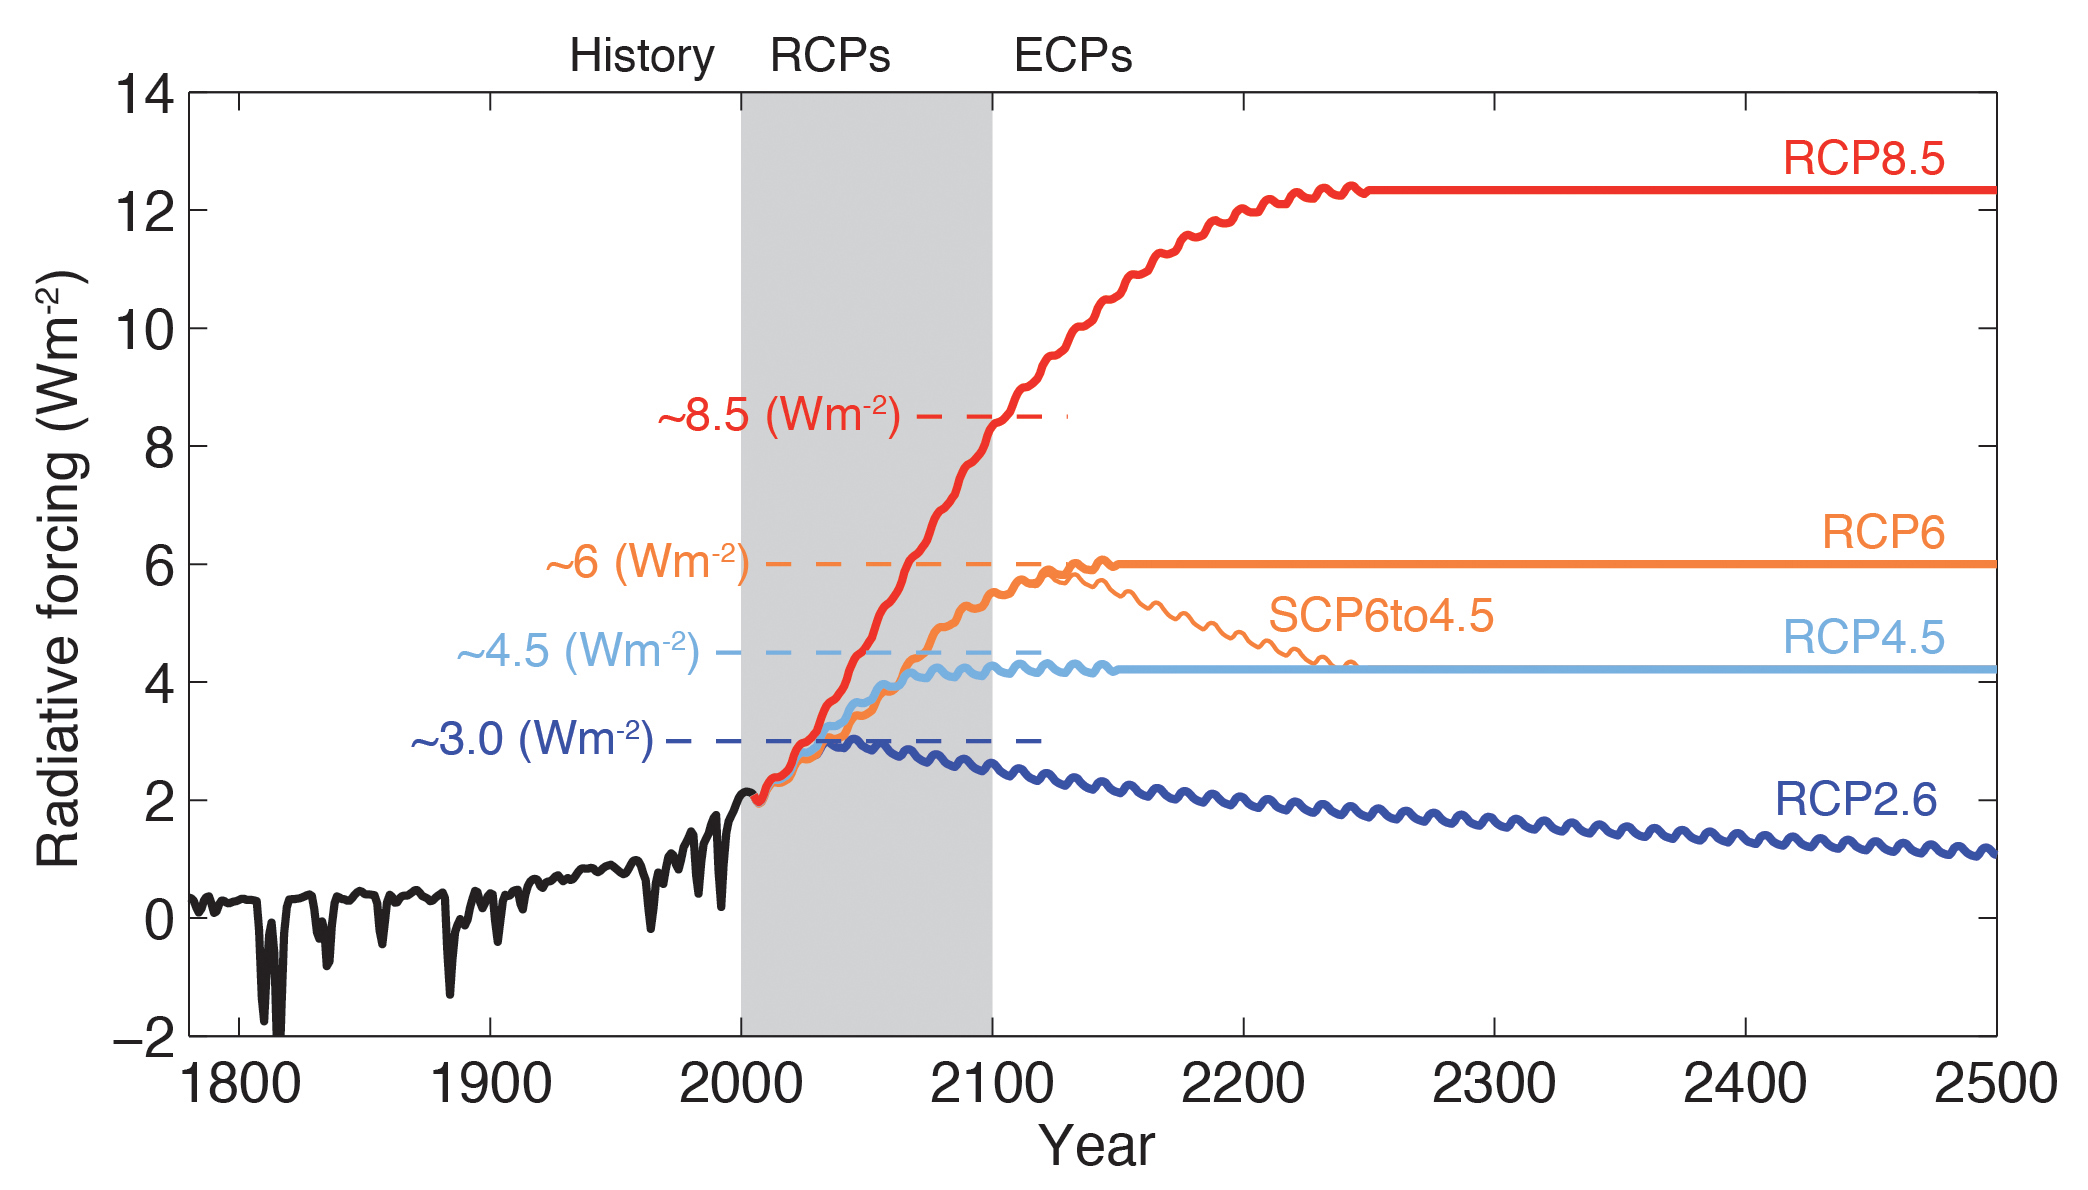
\includegraphics[width=0.55\textwidth]{Figures/Outlook/IPCC_RCP_ECP.jpg}
	};
	\node[xshift=-3cm,yshift=-2cm] at (current page.center) {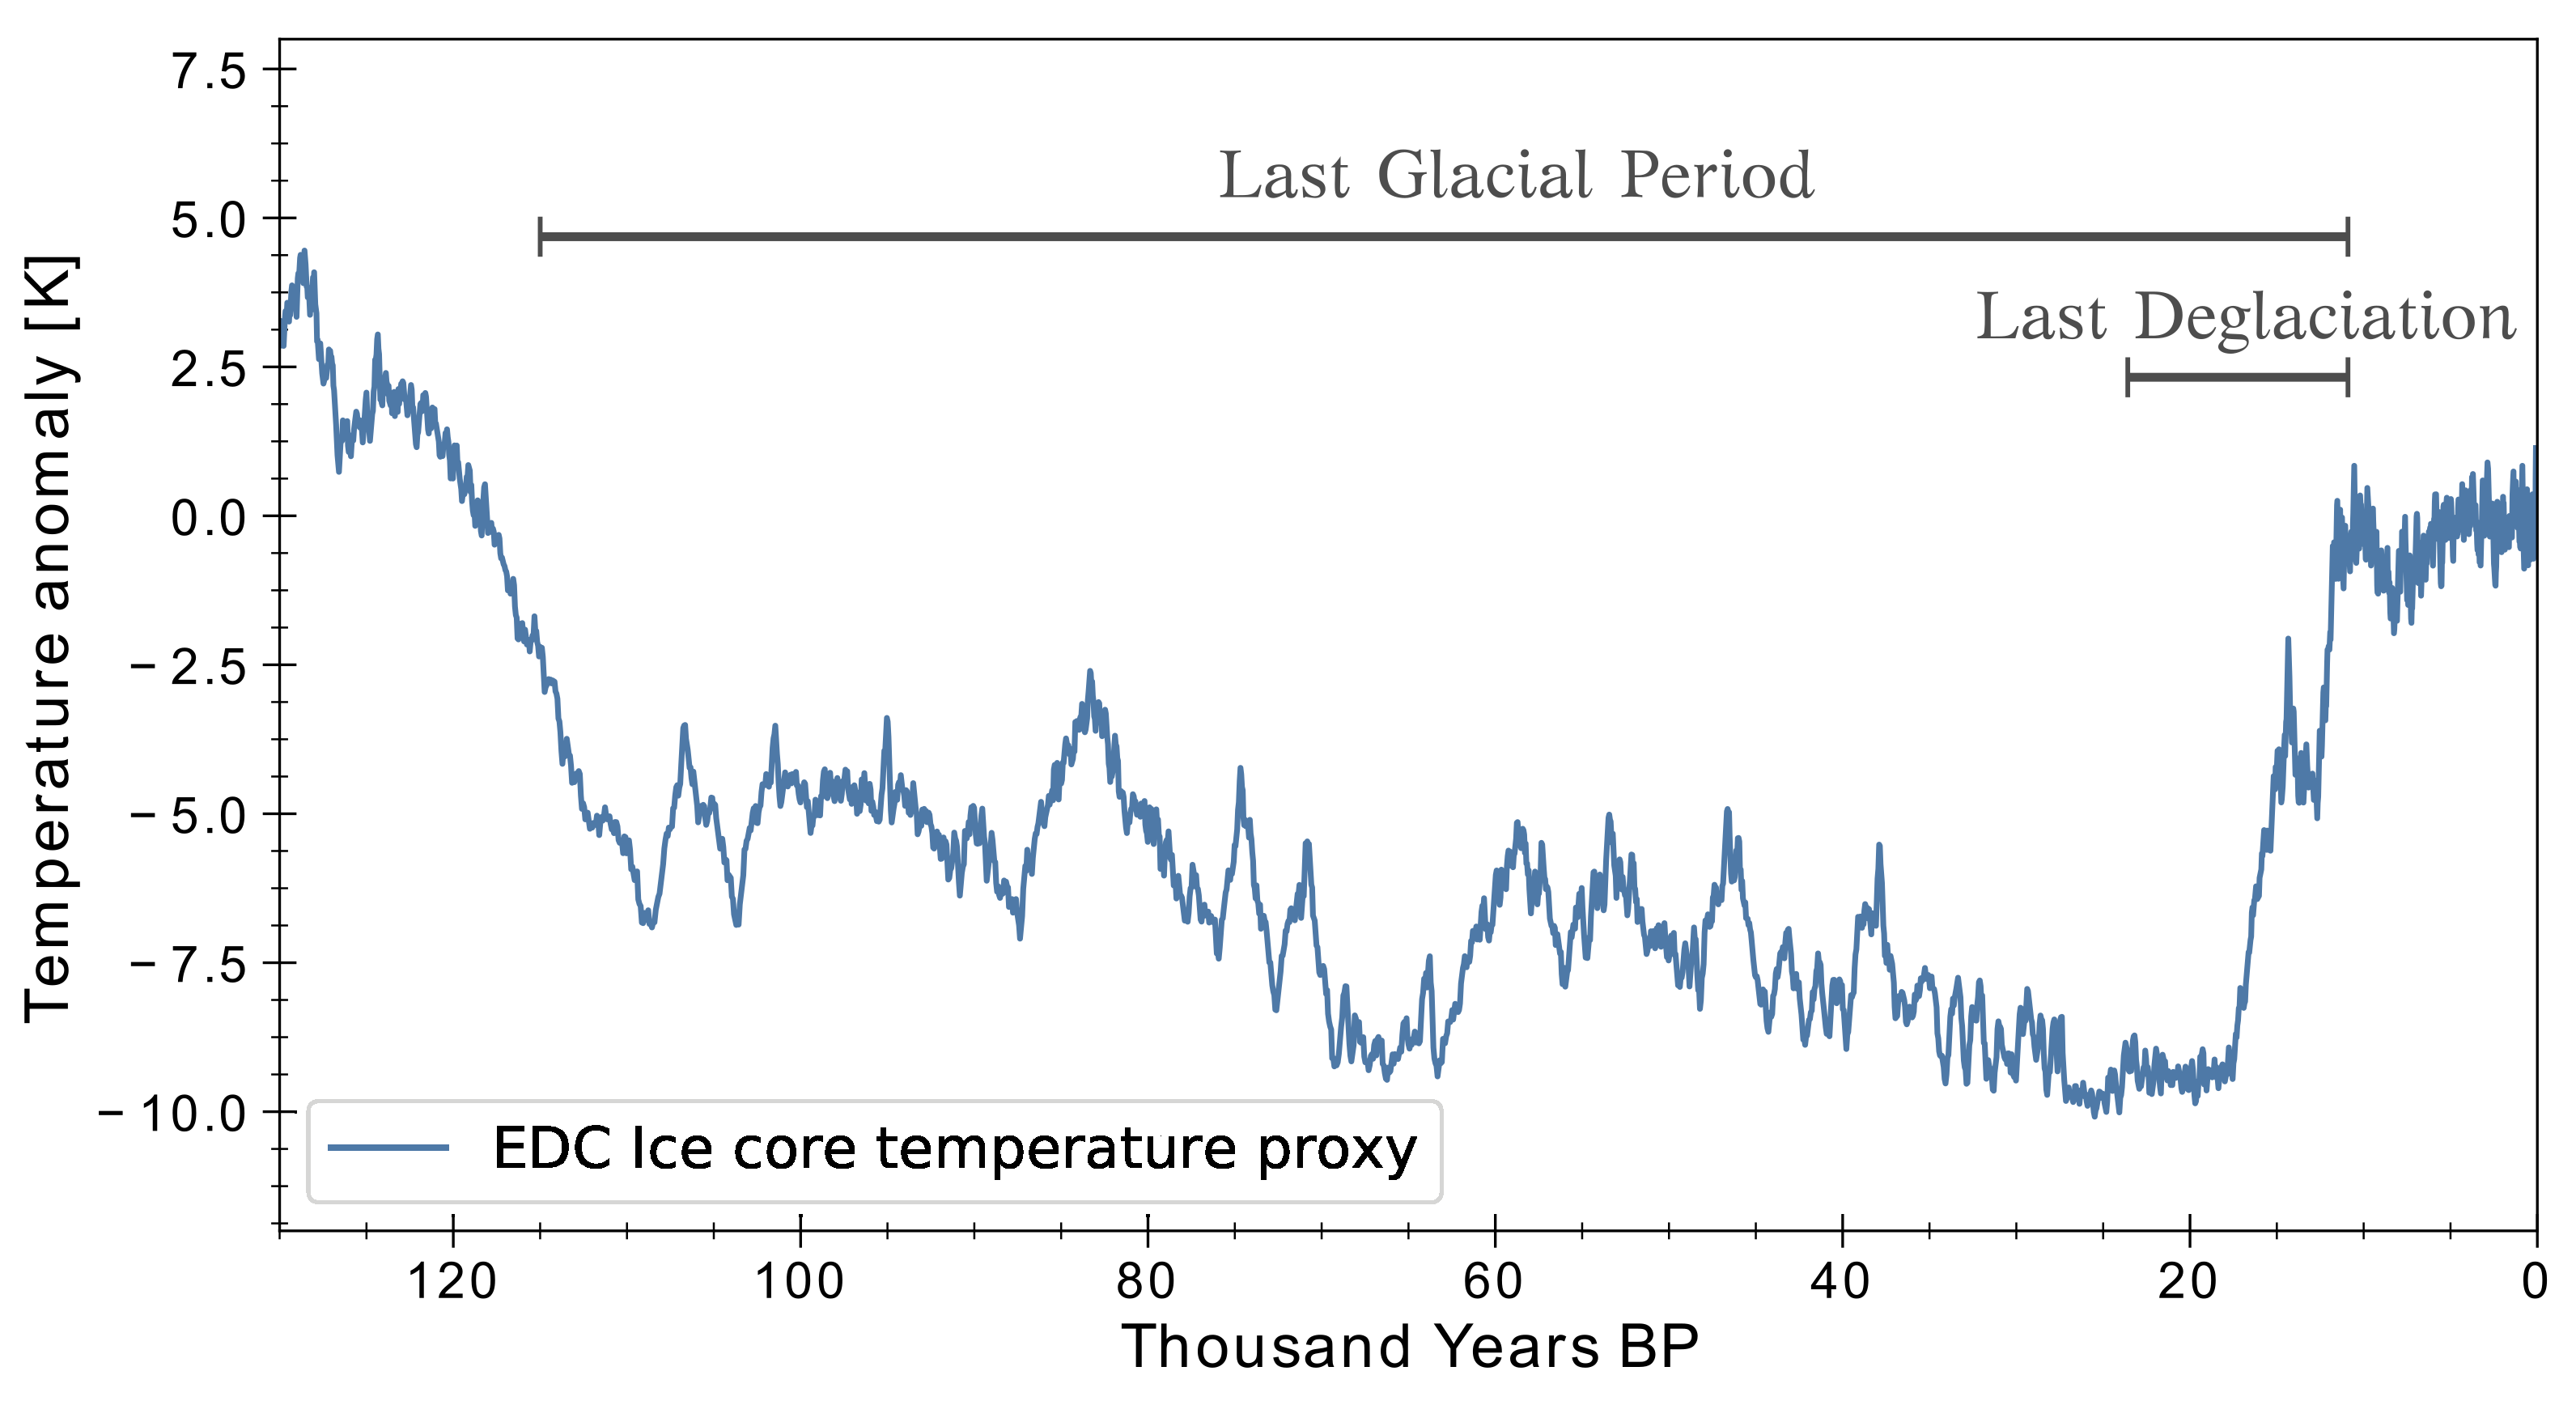
\includegraphics[width=0.55\textwidth]{Figures/Outlook/Deglaciation.png}
	};
	\end{tikzpicture}
	\blfootnote{[IPCC 2013, Jouzel 2007]}
\end{frame}

\begin{frame}
	\begin{tikzpicture}[remember picture,overlay]
	\node[align=left,anchor=west,xshift=-4.7cm,yshift=1cm] at (current page.center) {\huge{Thank you for your attention!}};
	\renewcommand*{\UrlFont}{\ttfamily\smaller\relax}
	\node[align=center,anchor=west,xshift=-5.2cm,yshift=-3cm] at (current page.center) {\normalsize If you are interested in details:\\ \url{https://github.com/BenniSchmiedel/Low-dimensional-EBMs}\\ or\; \url{https://lowebms.readthedocs.io/en/latest/} };
	\end{tikzpicture}
\end{frame}

\begingroup
\scriptsize
\begin{frame}{Referenzen}
\begin{flushleft}
\begin{itemize}
\item M. I. Budyko, G. Observatory, and M. Spasskaja: The effect of solar radiation variations on the climate of
the Earth. Tellus XXI (1969), 7, 1968.
\item W. D. Sellers: A Global Climatic Model Based on the Energy Balance of the Earth-Atmosphere Sys-
tem. Journal of Applied Meteorology, 8(3):392–400, 1969.
\item IPCC: Climate Change 2013 - The Physical Science Basis. Cambridge University Press, Cambridge, 2013.
\item M. Toohey, B. Stevens, H. Schmidt and C. Timmreck: Easy Volcanic Aerosol (EVA v1.0): an idealized forcing generator for climate simulations. Geosci. Model Dev., 2016.
\item T. J. Crowley et al.: Volcanism and the Little Ice Age. PAGES News, April 2008.
\item F. Steinhilber, J. Beer, and C. Fröhlich: Total solar irradiance during the Holocene. Geophysical Research Letters, 2009.
\item G. R. North and K. Kwang-Yul: Energy Balance Climate Models. Wiley-VCH Verlag GmbH \& Co. KGaA,
2017.
\item T. Stocker: Introduction to Climate Modelling. Springer Berlin Heidelberg, 2011.
\item K. McGuffie and A. Henderson-Sellers: The Climate Modelling Primer. Wiley-Blackwell, 2014.
\item J. Jouzel et al.: Orbital and Millennial Antarctic Climate Variability over the Past 800,000 Years. Science, 2007.
\end{itemize}
\end{flushleft}
\end{frame}
\endgroup

\begingroup
\small
\begin{frame}[noframenumbering]
\begin{tabular}{l|| l l l l l l}
        Parameter & $A_0$ & $B_0$ & $ A_1$ & $B_1$ & n & $\beta$\\\hline
        Value & 222.74 $\frac{W}{m^2}$ & 2.23 $\frac{W}{m^2K}$ & 47.73 $\frac{W}{m^2}$ & 1.59 $\frac{W}{m^2K}$ & 0.5 & 3.74 $\frac{W}{m^2K}$
\end{tabular}
\begin{align*}
&R(t)_{in,i} = Q_i\cdot(1-\alpha_i(T))\\
&R(t)_{out,i}  = A_0+B_0 T(t)_i - n\cdot(A_1+B_1 T(t)_i)\\
&F(t)_{transfer,i}  =  \beta\cdot(T_i (t) - T_p (t))
\end{align*}
\end{frame}

\begin{frame}[noframenumbering]
\begin{align*}
&R(t)_{in,i} =  Q_i\cdot(1-\alpha_i)\\
&R(t)_{out,i}  =  \sigma T^4(t)_i (1-m\cdot \tanh{(\gamma T^6(t)_i)})\\
&F(t)_{transfer,i}  =  (P(t)_i l_i-P(t)_{i+1} l_{i+1})/ A_i\\
&P_i=  L\,c(t)_i+C(t)_i+F(t)_{ocean,i}\\
&c=\left(vq-K_w\frac{\Delta q}{\Delta y}\right)\frac{\Delta p}{g}\\
&C=\left(vT-K_h\frac{\Delta T}{\Delta y}\right) \frac{c_p}{g}\Delta p\\
&F_{ocean,i}=-K_o \Delta z \frac{l'}{l} \frac{\Delta T}{\Delta y} c_{p,w} \rho_w\\
\end{align*}
\end{frame}

\begin{frame}[noframenumbering]
\begin{align*}
&v=-a(\Delta T\pm |\overline{\Delta T}|)\\
&q=\frac{\epsilon e}{p}\\
&\Delta q =\frac{\epsilon^2 Le\Delta T}{p R_d T_0^2}\\
&e =  e_0 \left(1 - 0.5\frac{\epsilon L \Delta T }{R_d T_0^2}\right)
\end{align*}
\end{frame}

\begin{frame}[noframenumbering]
\begin{tabular}{l|l}\hline\hline
Description & Value\\\hline\hline
\underline{$R_{out}$} & \\
m & 0.5 \\
$\sigma$ & $5.67\cdot 10^{-8}$ $W/(m^2 K^4)$ \\
$\gamma$ & $1.9 \cdot 10^{-15} $ $1/T^6$\\\hline
\underline{$F_{transfer}$} & \\
g & 9.81 $m/s^2$ \\
$\epsilon$ & 0.622 \\
p & 1000 $mb$ \\
$e_0$ & 17 $mb$ \\
L &  $2.5\cdot 10^3$ $J/g$ \\
$R_d$ & 0.287 $J/(g K)$\\
$\Delta y$ & $1.11\cdot10^6 m$ \\
$c_p$ & 1.004 $J/(g K)$\\
l' & 0.5 \\
$c_{p,w}$ & 4.182 $J/(kg K)$\\
$\rho_w$ & 997 $kg / m^3$
\end{tabular}
\end{frame}

\end{document}